\chapter{Variational Inference for GW Parameter Estimation}\label{ch:chap_5}

We note to the reader that this text is a modified version of the 
paper under review here~\cite{1909.06296}. 

So far, we have introduced fundamental 
concepts from \ac{GW} astronomy and \ac{ML}. We have also provided 
a broad survey of how \ac{ML} is being applied across a variety of 
domains within \ac{GW} astronomy. In the previous chapter (Ch.~\ref{ch:chap_4})
we showed one 
of the first implementations of deep learning for \ac{GW} signal 
detection and how our approach was able to match the sensitivies 
of standard methods, opening the door for a variety of follow-up 
studies listed in Ch.~\ref{ch:chap_3}. We now move on to the more 
challenging task of applying \ac{ML} methods towards \ac{GW} Bayesian 
parameter estimation. We show for the first time that a form of 
\ac{ML}, variational inference, may be used to produce Bayesian posteriors 
of \ac{GW} source parameter values given \ac{GW} time series data in 
a fraction of the time taken by more traditional samplers.

\section{Introduction}

%
% background
%
\ac{GW} detection is now commonplace~\cite{PhysRevX.6.041015,PhysRevLett.119.161101} and as 
the sensitivity of the global network of \ac{GW} detectors 
improves, we will observe $\mathcal{O}(100)$s of transient 
\ac{GW} events per year~\cite{2018LRR....21....3A,1304.0670,1811.12907}. The current 
methods used to estimate their source parameters employ 
optimally sensitive~\cite{2009CQGra..26o5017S} but computationally 
costly Bayesian inference approaches~\cite{1409.7215} where typical 
analyses have taken between 6 hours and 38 days~\cite{gracedb_O3} to run. We 
determined these values by 
compiling tables (Tab.~\ref{tab:o3_events_runtime_1} 
and Tab.~\ref{tab:o3_events_runtime_2}) containing of all 
detected events during the O3 observing 
run using the GraceDB database. We provide in the tables the length of 
time to complete parameter estimation analyses using the lalinference 
pipeline~\cite{1409.7215}, as well as the predicted source 
class using the \texttt{p-astro}~\footnote{See  
\url{https://pypi.org/project/p-astro/}.} computing package.
~\chris{Maybe even make a plot of run time vs total inferred mass and runtime vs SNR.}.

%
% O3 detected events table 1
%
\begin{sidewaystable}
\centering
\caption[O3 events table containing information on detected event 
parameter estimation runtimes from April 8, 2019 - September 10, 
2019]{O3 events 
table containing information on detected event parameter estimation 
runtimes and classification 
probability (according to GraceDB) from April 8, 2019 - September 10, 
2019. The amount of 
time for a run to produce 
final parameter estimation results is given by the difference between the 
event time and the first reported parameter estimation results from 
lalinference. We do not show here any detection events flagged 
by GraceDB that were later retracted. Columns with a ``-'' are values 
which were either not reported by GraceDB, or could not be found.}
\resizebox{21cm}{!}{
\begin{tabular}{l*{6}{c}r}~\label{tab:o3_events_runtime_1}
\\
\hline
Event Name & Classification & Event Time & First LAL Results & Results Delay \\
\hline
\hline
S190408an & BBH ($>99\%$) & April 8, 2019 18:18:02 UTC & 2019-04-14 05:37:36 UTC & 5 d, 11 hrs, 19 min, 34 s \\
\hline
S190412m & BBH ($>99\%$) & April 12, 2019 05:30:44 UTC & - & - \\
\hline 
S190421ar & BBH ($97\%$), & April 21, 2019 21:38:56 UTC & 
May 3, 2019 08:18:56 UTC & 11 d, 10 hrs, 40 mins, 0 s \\
& Terrestrial ($3\%$) & & & \\
\hline 
S190425z & BNS ($>99\%$) & April 25, 2019 08:18:05 UTC & 
Apr 26, 2019 11:02:22 UTC & 1 d, 2 hrs, 44 mins, 17 s \\
\hline 
S190426c & BNS ($49\%$), MassGap ($24\%$), & 
April 26, 2019 15:21:55 UTC & Apr 28, 2019 17:11:32 UTC & 
2 d, 1 hr, 49 min, 37 s \\ 
& Terrestrial ($14\%$), NSBH ($13\%$) & & & \\ 
\hline 
S190503bf & BBH ($96\%$), MassGap ($3\%$) & May 3, 2019 18:54:04 UTC & 
Jun 11, 2019 08:18:41 UTC & 38 d, 13 hrs, 24 min, 37 s \\
\hline 
S190510g & Terrestrial ($58\%$), BNS ($42\%$) & May 10, 2019 02:59:39 UTC & 
Jun 3, 2019 16:19:23 UTC & 24 d, 13 hrs, 19 min, 44 s \\
\hline 
S190512at & BBH ($99\%$), Terrestrial ($1\%$) & May 12, 2019 18:07:14 UTC 
& May 17, 2019 15:27:36 UTC & 4 d, 21 hrs, 20 min, 22 s \\
\hline
S190513bm & BBH ($94\%$), MassGap ($5\%$) & May 13, 2019 20:54:28 UTC & 
May 16, 2019 14:43:37 UTC & 2 d, 17 hrs, 49 min, 9 s \\
\hline
S190517h & BBH ($98\%$), MassGap ($2\%$) & May 17, 2019 05:51:01 UTC & 
May 21, 2019 15:22:31 UTC & 4 d, 9 hrs, 31 min, 30 s \\
\hline 
S190519bj & BBH ($96\%$), Terrestrial ($4\%$) & May 19, 2019 15:35:44 UTC 
& May 22, 2019 10:05:27 UTC & 2 d, 18 hrs, 29 min, 43 s \\
\hline 
S190521g & BBH ($97\%$), Terrestrial ($3\%$) & May 21, 2019 03:02:29 UTC
& May 21, 2019 09:11:04 UTC & 0 d, 6 hrs, 8 min, 35 s \\
\hline 
S190521r & BBH ($>99\%$) & May 21, 2019 07:43:59 UTC & 
May 24, 2019 21:22:47 UTC & 3 d, 13 hrs, 38 min, 48 s \\ 
\hline 
S190602aq & BBH ($99\%$) & June 2, 2019 17:59:27 UTC & 
Jun 7, 2019 14:21:51 UTC & 4 d, 20 hrs, 22 min, 24 s \\
\hline
S190630ag & BBH ($94\%$), MassGap ($5\%$) & June 30, 2019 18:52:05 UTC 
& Jul 1, 2019 18:09:39 UTC & 0 d, 23 hrs, 17 min, 34 s \\
\hline
S190701ah & BBH ($93\%$), Terrestrial ($7\%$) & 
July 1, 2019 20:33:06 UTC & Jul 3, 2019 02:08:14 UTC & 1 d, 5 hrs, 
35 min, 8 s \\ 
\hline
S190706ai & BBH ($99\%$), Terrestrial ($1\%$) & 
July 6, 2019 22:26:41 UTC & Jul 8, 2019 05:17:16 UTC & 1 d, 6 hrs, 50 min, 
35 s \\
\hline
S190707q & BBH ($>99\%$) & July 7, 2019 09:33:26 UTC & 
Jul 9, 2019 17:48:32 UTC & 2 d, 8 hrs, 15 min, 6 s \\
\hline
S190718y & Terrestrial ($98\%$), BNS ($2\%$) & July 18, 2019 14:35:12 UTC 
& - & - \\
\hline
S190720a & BBH ($99\%$), Terrestrial ($1\%$) & July 20, 2019 00:08:36 UTC & 
Jul 21, 2019 13:54:03 UTC & 1 d, 13 hrs, 45 min, 27 s \\
\hline
S190727h & BBH ($92\%$), Terrestrial ($5\%$), & July 27, 2019 06:03:33 UTC
& Jul 31, 2019 20:08:10 UTC & 4 d, 14 hrs, 4 min, 37 s \\
& MassGap ($3\%$) & & & \\
\hline
S190728q & BBH ($95\%$), MassGap ($5\%$) & July 28, 2019 06:45:10 UTC & 
Jul 30, 2019 10:32:36 UTC & 2 d, 3 hrs, 47 min, 26 s \\
\hline
S190814bv & NSBH ($>99\%$) & Aug. 14, 2019 21:10:39 UTC & 
Aug 15, 2019 09:02:34 UTC & 11 hrs, 51 min and 55 s \\
\hline
S190828j & BBH ($>99\%$) & Aug. 28, 2019 06:34:05 UTC & 
Aug 30, 2019 07:58:27 UTC & 2 d, 1 hr, 24 min and 22 s \\
\hline
S190828l & BBH ($>99\%$) & Aug. 28, 2019 06:55:09 UTC & 
Aug 29, 2019 15:43:57 UTC & 1 d, 8 hrs, 48 min and 48 s \\
\hline
S190901ap & BNS ($86\%$), Terrestrial ($14\%$) & 
Sept. 1, 2019 23:31:01 UTC & Sep 2, 2019 11:21:59 UTC & 
11 hrs, 50 min, 58 s \\
\hline
S190910d & NSBH ($98\%$), Terrestrial ($2\%$) & Sept. 10, 2019 01:26:19 UTC & 
Sep 10, 2019 22:33:57 UTC & 21 hrs, 7 min, 38 s \\
\end{tabular} 
}
\end{sidewaystable}

%
% O3 detected events table 2
%
\begin{sidewaystable}
\centering
\caption[O3 events table containing information on detected event 
parameter estimation runtimes from September 10, 2019 - March 16, 2020.]{
O3 events table containing information on detected event parameter 
estimation runtimes and classification 
probability (according to GraceDB) from September 10, 2019 - 
March 16, 2020. 
The amount of time for a run to produce 
final parameter estimation results is given by the difference between the 
event time and the first reported parameter estimation results from 
lalinference. We do not show here any detection events flagged 
by GraceDB that were later retracted. Columns with a ``-'' are values 
which were either not reported by GraceDB, or could not be found.}
\resizebox{21cm}{!}{
\begin{tabular}{l*{6}{c}r}~\label{tab:o3_events_runtime_2}
\\
\hline
Event Name & Classification & Event Time & First LAL Results & Results Delay \\
\hline
\hline
S190910h & BNS ($61\%$), Terrestrial ($39\%$) & 
Sept. 10, 2019 08:29:58 UTC & Sep 11, 2019 17:11:34 UTC & 
1 d, 8 hrs, 41 min, 36 s \\
\hline
S190915ak & BBH ($99\%$) & Sept. 15, 2019 23:57:02 UTC & 2019-09-17 13:42:31 UTC 
& 1 d, 13 hrs, 45 min, 29 s \\
\hline
S190923y & NSBH ($68\%$), Terrestrial ($32\%$) & 
Sept. 23, 2019 12:55:59 UTC & - & - \\
\hline
S190924h & MassGap ($>99\%$) & Sept. 24, 2019 02:18:46 UTC & 
2019-09-27 19:17:41 UTC & 3 d, 16 hrs, 58 min, 55 s \\
\hline
S190930s & MassGap ($95\%$), Terrestrial ($5\%$) & 
Sept. 30, 2019 13:35:41 UTC & 2019-10-04 19:25:05 UTC & 
4 d, 5 hrs 49 min, 24 s \\
\hline
S190930t & NSBH ($74\%$), Terrestrial ($26\%$) & 
Sept. 30, 2019 14:34:07 UTC & - & - \\
\hline
S191105e & BBH ($95\%$), Terrestrial ($5\%$) & 
Nov. 5, 2019 14:35:21 UTC & 2019-11-12 12:51:56 UTC & 
6 d, 22 hrs, 16 min, 35 s \\
\hline
S191109d & BBH ($>99\%$) & Nov. 9, 2019 01:07:17 UTC & 
2019-11-10 14:31:40 UTC & 1 d, 13 hrs, 24 min, 23 s \\
\hline
S191129u & BBH ($>99\%$) & Nov. 29, 2019 13:54:17 UTC & 
2019-12-05 13:54:17 UTC & 6 d, 13 min, 48 s \\
\hline
S191204r & BBH ($>99\%$) & Dec. 4, 2019 17:15:26 UTC & - & - \\
\hline
S191205ah & NSBH ($93\%$), Terrestrial ($7\%$) & 
Dec. 5, 2019 21:52:08 UTC & - & - \\
\hline
S191213g & BNS ($77\%$), Terrestrial ($23\%$) & 
Dec. 13, 2019 04:34:08 UTC & - & - \\
\hline
S191215w & BBH ($>99\%$) & 
Dec. 15, 2019 22:30:52 UTC & 2019-12-20 09:18:36 UTC & 4 d, 
10 hrs, 47 min, 44 s \\
\hline
S191216ap & BBH ($99\%$) & Dec. 16, 2019 21:33:38 UTC & - & - \\
\hline
S191222n & BBH ($>99\%$) & Dec. 22, 2019 03:35:37 UTC & 2019-12-22 22:06:36 UTC 
& 18 hrs, 30 min, 59 s \\
\hline
S200105ae & Terrestrial ($97\%$), NSBH ($3\%$) & Jan. 5, 2020 16:24:26 UTC
& 2020-01-09 16:56:28 UTC & 4 d, 32 min, 2 s \\
\hline
S200112r & BBH ($>99\%$) & Jan. 12, 2020 15:58:38 UTC & 2020-01-14 15:54:35 UTC 
& 1 d, 23 hrs, 55 min, 57 s \\
\hline
S200114f & - & Jan. 14, 2020 02:08:18 UTC & - & - \\
\hline
S200115j & MassGap ($>99\%$) & Jan. 15, 2020 04:23:09 UTC & 
2020-01-20 04:51:25 UTC & 5 d, 28 min, 16 s \\
\hline 
S200128d & BBH ($97\%$), Terrestrial ($3\%$) & Jan. 28, 2020 02:20:11 UTC 
& 2020-01-30 09:35:52 UTC & 2 d, 7 hrs, 15 min, 41 s \\ 
\hline 
S200129m & BBH ($>99\%$) & Jan. 29, 2020 06:54:58 UTC & 
2020-02-03 00:08:54 UTC & 4 d, 17 hrs, 13 min, 56 s \\
\hline
S200208q & BBH ($99\%$) & Feb. 8, 2020 13:01:17 UTC & 2020-02-10 21:01:12 UTC 
& 2 d, 7 hrs, 59 min, 55 s \\
\hline
S200213t & BNS ($63\%$), Terrestrial ($37\%$) & Feb. 13, 2020 04:10:40 UTC 
& - & - \\
\hline
S200219ac & BBH ($96\%$), Terrestrial ($4\%$) & Feb. 19, 2020 09:44:15 UTC 
& - & - \\
\hline
S200224ca & BBH ($>99\%$) & Feb. 24, 2020 22:22:34 UTC & 
2020-02-26 13:49:38 UTC &  1 d, 15 hrs, 27 min, 4 s \\ 
\hline
S200225q & BBH ($96\%$), Terrestrial ($4\%$) & Feb. 25, 2020 06:04:21 UTC 
& 2020-02-26 07:42:24 UTC & 1 d, 1 hrs, 38 min, 3 s \\
\hline
S200302c & BBH ($89\%$), Terrestrial ($11\%$) & March 2, 2020 01:58:11 UTC 
& 2020-03-02 19:06:13 UTC & 17 hrs, 8 min, 2 s \\
\hline
S200311bg & BBH ($>99\%$) & March 11, 2020 11:58:53 UTC & 
2020-03-13 04:55:55 UTC & 1 d, 16 hrs, 57 min, 2 s \\
\hline
S200316bj & MassGap ($>99\%$) & March 16, 2020 21:57:56 UTC & 
2020-03-21 02:46:41 UTC & 4 d, 4 hrs, 48 min, 45 s \\
\hline
\end{tabular}    
}
\end{sidewaystable}

%
% rationale
%
For \ac{BNS} and \ac{NSBH} systems prompt counterpart \ac{EM} signatures are expected on timescales of 1~s -- 1~minute and the current fastest method for alerting \ac{EM} follow-up observers~\cite{2016PhRvD..93b4013S}, can provide estimates in $\mathcal{O}(1)$ minute, on a limited range of key source parameters~\chris{You could rephrase to refer to O3 results only and use the gracedb website to verify these low latency times - also include them in the table.}. 
%
% results
%
Here we show that a \ac{CVAE}~\cite{1904.06264,1812.04405} pre-trained 
on \ac{BBH} signals can return Bayesian posterior probability estimates. 
The training procedure need only be performed once for a given 
prior parameter space and detector network configuration and the 
resulting trained machine can then generate samples describing the 
posterior distribution $\sim 6$ orders of magnitude faster 
than existing techniques.

%%%%%%%%%%%%%%%%%%%%%%%%%%%%%%%%%%%%%%%%%%%%%%%%%%%%%%%%%%%%%%%%%%%%%%
% INTRODUCTION
%%%%%%%%%%%%%%%%%%%%%%%%%%%%%%%%%%%%%%%%%%%%%%%%%%%%%%%%%%%%%%%%%%%%%%
%
% introduction - this section has to expand upon what has mentioned in the
% abstract background (which was only ~50 words). It needs to cover the state of
% the gravitational wave field and the number of detections expected in the next
% ~5 years. It should briefly discuss the issue of low latency EM follow up. It
% needs to cover Bayesian inference (not in too much detail) and the signal model
% we are interested in here (again, not too much detail but enough for the
% average Nature reader). It then needs to introduce machine learning and focus
% mainly on how our scheme works. We also need to include a statement about how
% the training data priors affect the result (are they really the priors?)
%
% Intro to the detection era with the LVC
%
With the overwhelmingly successful observation runs of O1, O2 and now 
O3 complete, \ac{LIGO} and Virgo have produced a large catalogue of 
\ac{GW} data covering both \ac{BBH} and \ac{BNS} signals~\cite{2010.14527}. 
Over the next five years we expect the number of detections to 
increase to be upwards of $\sim180$ \ac{BNS} and $\sim400$ 
\ac{BBH} events per year~\cite{1304.0670,1811.12907,2018LRR....21....3A}. 
This large influx in the number of detections will put an 
increased amount of pressure on the current computationally 
costly \ac{GW} inference methods used for parameter estimation.  

%
% From GW detection, to parameter estimation
%

The problem of detecting \acp{GW}s has largely been solved through the 
use of template based matched-filtering, a process recently 
replicated using machine learning
techniques
~\cite{GEORGE201864,PhysRevLett.120.141103,
GebKilParHarSch,2021arXiv210403961Y}. Once a \ac{GW} has been 
identified through this process, Bayesian inference, known 
to be the optimal approach~\cite{2009CQGra..26o5017S}, is used to 
extract information about the source parameters of the detected \ac{GW} signal.

%
% Set up parameter estimation problem
%
In the standard Bayesian \ac{GW} inference approach (See 
Sec.~\ref{sec:bayesian_inference} of 
Ch.~\ref{ch:chap_1}), we assume a 
signal and noise model and both may have unknown parameters that we 
are either interested in inferring or prefer to marginalise away. Each 
parameter is given a prior astrophysically motivated probability 
distribution and in the \ac{GW} case, we
typically assume a Gaussian additive noise model (in reality, the d
ata is not truly Gaussian). Given a noisy \ac{GW} waveform, 
we would like to find an optimal procedure for inferring 
some set of the unknown \ac{GW} parameters. Such a procedure 
should be able to give us an accurate estimate of the parameters 
of our observed signal, whilst accounting for the uncertainty 
arising from the noise in the data.

%
% Describe Bayes Theorem
%
According to Bayes' Theorem, a posterior probability distribution on a set of parameters, conditional on the measured data, can be represented as
%
\begin{align}\label{eq:bayes_theorem} 
p(x|y) &\propto p(y|x) p(x), 
\end{align}
%
where $x$ are the parameters, $y$ is the observed data, 
$p(x|y)$ is the posterior, $p(y|x)$ is 
the likelihood, and $p(x)$ is the prior on the parameters. The 
constant of proportionality, which we omit here, is $p(y)$, the 
probability of our data, known as the Bayesian evidence or the 
marginal likelihood. We typically ignore $p(y)$ since it is a constant 
and for parameter estimation purposes we are only interested in the 
shape of the posterior (See Sec.~\ref{sec:bayesian_inference} of 
Ch.~\ref{ch:chap_1} for further details).

%
% brief statement on the sampling algorithms
%
Due to the size, dimensionality and volume of the parameter 
space typically encountered in \ac{GW} parameter estimation and the 
volume of data analysed, we must stochastically sample the 
parameter space in order to estimate the posterior. Sampling is 
done using a variety of techniques including Nested
Sampling~\cite{skilling2006,cpnest,dynesty} and Markov chain 
Monte Carlo methods~\cite{emcee,ptemcee}. The primary software 
tools used by the \ac{LIGO} parameter estimation analysis 
are \texttt{LALInference} and
\texttt{Bilby}~\cite{1409.7215,1811.02042}, which offer 
multiple sampling methods.  
  
%
% Intro to machine learning section
%
Machine learning has featured prominently in many areas of 
\ac{GW} research over the last few years. These techniques have 
shown to be particularly promising in signal
detection~\cite{GEORGE201864,PhysRevLett.120.141103,GebKilParHarSch},
glitch classification~\cite{0264-9381-34-6-064003}, earthquake
prediction~\cite{Coughlin_2017}, and to augment existing 
Bayesian sampling methods~\cite{10.1111/j.1365-2966.2011.20288.x}.
We also highlight recent developments in \ac{GW} parameter 
estimation (independent to this work) where one- and two-dimensional 
marginalised Bayesian posteriors are produced rapidly using 
neural networks~\cite{2019arXiv190905966C}, and where 
normalised flows in conjunction with \acp{CVAE} can reproduce 
Bayesian posteriors for a single \ac{GW} detector
case~\cite{PhysRevD.102.104057,2008.03312}. These methods, 
including the one presented in this paper, are known as 
``likelihood-free'' approaches in which there is no requirement for 
explicit likelihood evaluation~\cite{Cranmer201912789}, only 
the need to sample from the likelihood. Nor is it the case that 
pre-computed posterior distributions are required in the training procedure.

%
% Introduce CVAEs
%
Recently, a type of neural network known as \ac{CVAE} was shown to 
perform exceptionally well when applied towards computational 
imaging inference~\cite{1904.06264,NIPS2015_5775}, text to 
image inference~\cite{1512.00570}, high-resolution synthetic 
image generation~\cite{1612.00005}, 
end-to-end text-to-speech synthesis~\cite{2021arXiv210606103K}, and the fitting of incomplete 
heterogeneous data~\cite{1807.03653}. \acp{CVAE}, as part of the variational 
family of inference techniques are ideally suited to the 
problem of function approximation and have the potential to 
be significantly faster than existing
approaches. It is therefore this type of \ac{ML} 
network that we apply in the \ac{GW} case to accurately 
approximate the Bayesian posterior
$p(x|y)$, where $x$ represents the physical parameters that govern the \ac{GW} signal, 
and are the quantities we are interested in inferring. The data $y$ represents the 
noisy measurement containing the \ac{GW} signal and obtained from a network of \ac{GW} detectors. 

%
% Brief introduction to loss functions used in the neural networks
%
The construction of a \ac{CVAE} begins with the definition 
of a quantity to be minimised (referred to as a cost, or loss function). In 
our case we take the expectation over the cross entropy
%
\begin{align}\label{eq:cross_ent} 
H(p,r) &= - \left \langle \int dx\, p(x|y) \log r_{\theta}(x|y) \right \rangle 
\end{align}
%
between the true posterior $p(x|y)$ and 
$r_{\theta}(x|y)$, the parametric distribution that 
we will use neural networks to model and which we aim to be equal to 
the true posterior. The expectation value is taken over different realisations of signal 
and noise, $y$. The parametric model is
constructed from a combination of 2 (encoder and decoder) neural networks $r_{\theta_1}(z|y)$ and $r_{\theta_2}(x|y,z)$ where
%
\begin{align}\label{eq:latent_model}
r_{\theta}(x|y) = \int dz\,r_{\theta_1}(z|y)r_{\theta_2}(x|y,z).
\end{align}
%
In this case the $\theta$ subscripts represent sets of trainable neural network parameters and 
the variable $z$ represents locations within a \emph{latent space}. This latter object is 
typically a lower dimensional space within which an encoder can represent the input 
data, and via marginalisation 
over $z$ allows the construction of a rich family of possible probability densities of $x$.

Starting from Eq.~\ref{eq:cross_ent} it is possible to derive a computable bound for 
the cross-entropy that is reliant on the $r_{\theta_1}$ and $r_{\theta_2}$ 
networks and a third ``recognition'' encoder
network $q_{\phi}(z|x,y)$ governed by the trainable parameter-set $\phi$. 
The details of the derivation are described in the cost function derivation section 
(Sec.~\ref{sec:vit_cost_derivation}) and in~\cite{1904.06264} but equate to an 
optimisation of the \ac{ELBO}. The final form of the cross-entropy 
cost function is given by the bound
%
\begin{align}\label{eq:cost3} H \lesssim
\frac{1}{N}\sum_{n=1}^{N_{\text{b}}}\Big[\overbrace{-\log
r_{\theta_{2}}(x_{n}|z_{n},y_{n})}^{L}
+\overbrace{\text{KL}\left[q_{\phi}(z|x_{n},y_{n})||r_{\theta_{1}}(z|y_{n})\right]}^{\text{KL}}\Big],
\end{align}
%
which is also represented graphically in Fig.~\ref{fig:network_config}. The cost 
function is composed of 2 terms, the ``reconstruction'' cost $L$ which is a 
measure of how well the decoder network $r_{\theta_2}$ predicts the true signal 
parameters $x$, and the \ac{KL}-divergence cost that measures the similarity 
between the latent space distributions modelled by the $r_{\theta_1}$ and $q_{\phi}$ 
encoder networks. In practice, for each iteration of the training procedure, the 
integrations over $x,y$ and $z$ are approximated by a sum over a
batch of $N_{\text{b}}$ draws from the user defined prior $p(x)$, 
the known likelihood $p(y|x)$, and the recognition function 
$q_{\phi}(z|,x,y)$. Details of the training procedure are given in 
Sec.~\ref{sec:training_procedure}.  

%
% brief mention of differences to a standard CVAE
%
The implementation of the \ac{CVAE} that we employ in this chapter has 
a number of specific 
features that were included in order to tailor the analysis to \ac{GW} signals. 
The details of these enhancements are described in the network design 
(Sec.~\ref{sec:network_design}), training procedure
(Sec.~\ref{sec:training_procedure}), data augmentation
(Sec.~\ref{sec:vit_data_aug}), and phase/polarisation angle reparameterisation 
(Sec.~\ref{sec:phipsi_repar}) 
sections but in summary, the 
primary modifications are as follows, 1) Physically appropriate output decoder 
distributions are used for each output parameter: 
von Mises-Fisher distribution on the 
sky location parameters, von Mises distributions on all parameters 
with cyclic prior bounds,  
and truncated Gaussians for
parameters with defined prior bounds. 2) Each of the functions 
$r_{\theta_1},r_{\theta_2}$, and $q_{\phi}$ are modelled using deep 
convolutional neural networks with multi-detector timeseries represented as 
independent input channels. 3) The $r_{\theta_1}$ encoder models an $M=32$ 
component Gaussian mixture model within the $n_{z}=15$ 
dimensional latent space in 
order to capture the corresponding typical multi-modal
nature of \ac{GW} posterior
distributions. 4.) All cyclic parameters are represented as points 
in an abstract 2D plane. In the next section, we will now 
derive the cost function used 
to train the entire \ac{CVAE} outlined above.


\begin{figure}
    \begin{center}
    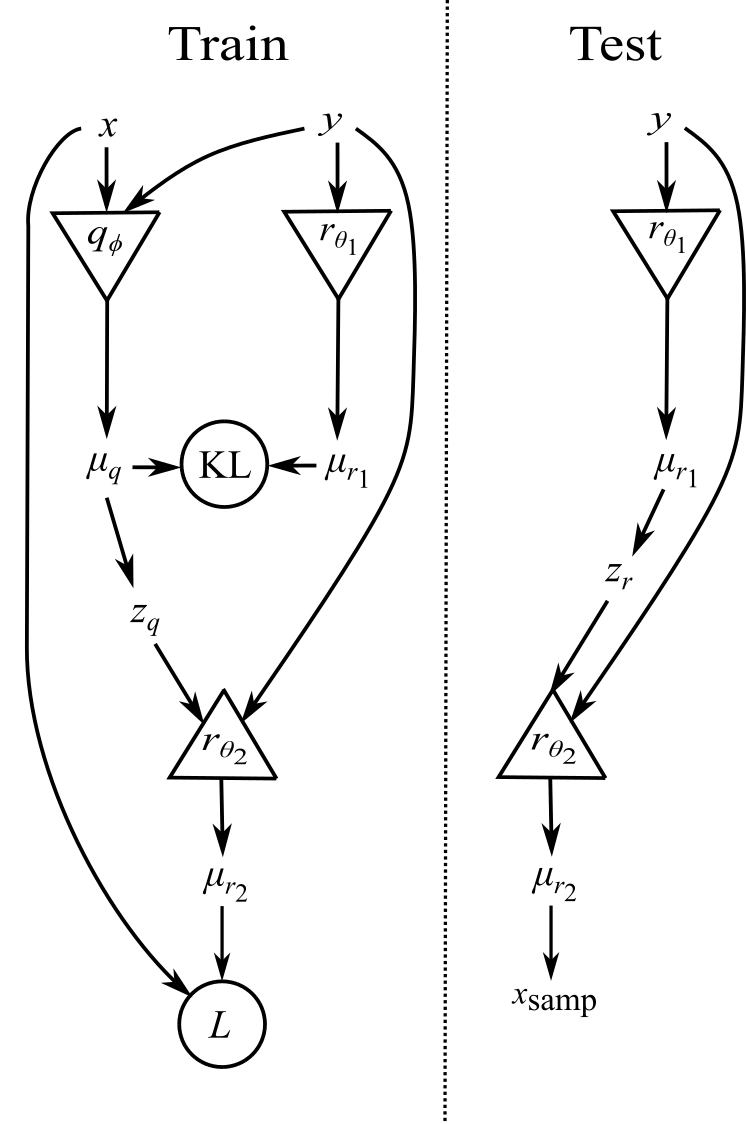
\includegraphics[width=0.75\columnwidth]{figures/network_setup.png}
    \caption{\label{fig:network_config} 
     The configuration of the \ac{CVAE} neural network. During training (left-hand side), a training set of noisy \ac{GW} signals ($y$) and their corresponding true parameters ($x$) are given as input to encoder network $q_{\phi}$, while only $y$ is given to encoder network $r_{\theta_1}$. The \ac{KL}-divergence (Eq.~\ref{eq:kl}) is computed between the encoder output latent space representations ($\mu_q$ and $\mu_r$) forming one component of the total cost function. Samples ($z_q$) from the $q_{\phi}$ latent space representation are generated and passed to the decoder network $r_{\theta_2}$ together with the original input data $y$. The output of the decoder ($\mu_x$) describes a distribution in the physical parameter space and the cost component $L$ is computed by evaluating that distribution at the location of the original input $x$. When performed in batches this scheme allows the computation of the total cost function Eq.~\ref{eq:cost3}. After having trained the network and therefore having minimised the cross-entropy $H$, the testing stage (right-hand side) is performed using only the $r_{\theta_1}$ encoder and the $r_{\theta_2}$ decoder to produce samples ($x_{\text{samp}}$). These samples are drawn from the distribution $r_{\theta}(x|y)$ (Eq.~\ref{eq:latent_model}) and accurately model the true posterior $p(x|y)$.}
    \end{center}
\end{figure}


%% Here is the endmatter stuff: Supplementary Info, etc.
%% Use \item's to separate, default label is "Acknowledgements"
%
% What is an autoencoder?
%
\section{VItamin Cost Function Derivation}\label{sec:vit_cost_derivation}
%
A \ac{CVAE} is a form of variational autoencoder that is conditioned on an observation, 
where in our case the observation is a one-dimensional \ac{GW} timeseries 
signal $y$, over a multi-detector network. The autoencoders from which variational 
autoencoders are derived are typically used for problems involving image reconstruction 
and/or dimensionality reduction. They perform a regression task whereby the 
autoencoder attempts to predict its own given input (model the identity function) through a 
``bottleneck layer'' --- a limited and therefore distilled representation of the input 
parameter space. An autoencoder is composed of two neural networks, an encoder and 
a decoder~\cite{gallinari1987memoires}. The encoder network takes as input a vector, where the 
number of dimensions is a fixed number predefined by the user. The encoder converts the 
input vector into a (typically) lower dimensional space, referred to as the 
{\it{latent space}}. A representation of the data in the latent space is passed to 
the decoder network which generates a reconstruction of the original input data to 
the encoder network. Through training, the two sub-networks learn how to efficiently 
represent a dataset within a lower dimensional latent space which will take on the most 
important properties of the input training data. In this way, the data can be compressed with 
little loss of fidelity. Additionally, the decoder simultaneously learns to decode the 
latent space representation and reconstruct that data back to its original form (the input data).

%
% What is a variational autoencoder?
%
The primary difference between a variational autoencoder~\cite{1812.04405} and an 
autoencoder concerns the method by which locations within the latent space are produced. 
In our variant of the variational autoencoder, the output of the encoder is interpreted 
as a set of parameters governing statistical
distributions in the latent space. In proceeding to the decoder network, samples 
from the latent space ($z$) are randomly drawn from these distributions and fed 
into the decoder, therefore adding an element of variation into the process. A particular 
input can then have a range of possible outputs. Any trainable network architectures 
can be used in both the decoder and the encoder networks and within 
\texttt{VItamin} we use deep convolutional neural networks in all cases.


%%%%%%%%%%%%%%%%%%%%%%%%%%%%%%%%%%%%%%%%%%%%%%%%%%%%%%%%%%%%%%%%%%%%%%
%
% Remind the reader about the point of the cost function 
%
We will now derive the cost function and the corresponding network structure and 
we begin with the statement defining the aim of the analysis. We wish to obtain a 
function that reproduces the posterior distribution (the probability of our 
physical parameters $x$ given some measured data $y$). The cross-entropy between 
2 distributions is defined in Eq.~\ref{eq:cross_ent} where we have made the 
distributions explicitly conditional on $y$ (our measurement). In this case 
$p(x|y)$ is the target distribution (the true posterior) and $r_{\theta}(x|y)$ is the 
parametric distribution that we will use neural networks 
to construct. The variable $\theta$ represents the trainable neural network parameters. 

%
% Marginalise over different data realisations 
%
The cross-entropy is minimised when $p(x|y)=r_{\theta}(x|y)$ and so by minimising
%
\begin{align}\label{eq:cost1}
H &= -\text{E}_{p(y)}\left[\int dx\,p(x|y) \log r_{\theta}(x|y)\right],
\end{align}
% 
where $\text{E}_{p(y)}[\cdot]$ indicates the expectation value over the 
distribution of measurements $y$, we therefore make the parametric distribution as 
similar as possible to the target for all possible measurements $y$.

%
% Use Bayes theorem to simplify
%
Converting the expectation value into an integral over $y$ weighted by $p(y)$ we get 
%
\begin{equation}
    H = -\int dy\,p(y) \int dx\,p(x|y) \log r_{\theta}(x|y).
\end{equation}
%
We then apply Bayes' theorem to obtain
\begin{equation}
    H = -\int dy\,p(y) \int dx\, \frac{p(y|x)p(x)}{p(y)} \log r_{\theta}(x|y)
\end{equation}
%
where $p(x)$ is the prior distribution on the physical parameters $x$, and $p(y|x)$ is the likelihood of $x$ (the probability of measuring the data $y$ given the parameters $x$).
Cancelling out the $p(y)$ terms we arrive at
%
\begin{align}\label{eq:cost1}
H &= -\int dx\,p(x)\int dy\,p(y|x)\log r_{\theta}(x|y).
\end{align}
%

%
% basic general description of the r1 and r2 network inputs and outputs
%
The \ac{CVAE} network outlined in Fig.~\ref{fig:network_config} makes use of a conditional 
latent variable model and our parametric model is constructed from the product of 2 
separate distributions marginalised over the latent space as defined in Eq.~\ref{eq:latent_model}. 
We have used $\theta_{1}$ and $\theta_{2}$ to indicate that the 2 separate networks 
modelling these distributions will be trained on these parameter sets respectively. 
The encoder $r_{\theta_1}(z|y)$ takes as input the data $y$ and outputs parameters 
that describe a probability distribution within the latent space. The decoder 
$r_{\theta_2}(x|z,y)$ takes as input a single location $z$ within the latent space 
together with the data $y$ and outputs sets of parameters describing a probability 
distribution in the physical parameter space.
%
% Explicitly describe mathematical form of 3 NN models
%
The explicit mathematical form $r_{\theta_2}(x|z,y)$ take is that of 
multiple multivariate Gaussian distributions whose moments, $\mu_{\mathrm{r}_2}$, are 
predicted by the parametric model given latent space samples $z$ and input data $y$.  
$r_{\theta_1}(z|y)$ takes the form of a Gaussian mixture 
model with a whose moments and mixture component weights (collectively labeled as 
$\mu_{\mathrm{r}_2}$) are also inferred by the parametric 
model given only observed data $y$.

%
% explain why we don't just stop here
%
One could be forgiven for thinking that by setting up networks that 
simply aim to 
minimise $H$ over the $\theta_{1}$ and $\theta_{2}$ would be 
enough to solve this 
problem. However, as shown in~\cite{NIPS2015_5775}, this 
is an intractable problem and a 
network cannot be trained directly to do this. Instead, we have 
to also train an additional network to approximate the theoretical 
joint probability distribution $r_{\theta}(z|x,y)$, which is essentially 
already defined by the existing $r_{\theta}(x|y)$, $r_{\theta_1}(z|y)$ 
and $r_{\theta_2}(x|z,y)$ joint distributions. We call the 
neural network which approximates the theoretical distribution,
 $r_{\theta}(z|x,y)$, the recognition 
function , $q_{\phi}(z|x,y)$, which is governed by the 
trainable network parameters, $\phi$, that will be used to derive an \ac{ELBO}. 
Furthermore, $q_{\phi}(z|x,y)$ takes the form of 
multiple multivariate Gaussian distributions 
whose moments, $\mu_{\mathrm{q}}$, are predicted by the parametric model given 
parameters $x$ and observed data $y$. It will become more clear in the 
derivation below that both defining and approximating this extra joint 
probability distribution is necessary because it allows us to define 
a computable form for $\log r_{\theta}(x|y)$. 

%
% define the ELBO
%
%We can derive an \ac{ELBO} by first recognising that decoder 
%$r_{\theta_2}(x|z,y)$ may be written as the following expression 
%using Bayes theorem and 
%Using Bayes theorem we can 
We first define the \ac{KL}-divergence between the recognition 
function and the distribution $r_{\theta}(z|x,y)$ as

%~\chris{for the paper this was fine but for the thesis I think you need to explain things a bit more. The reader will be confused as to where both of these distributions come from. they will also think that $r_{\theta}(z|x,y)$ is one of the other, already defined, $r$ distributions. The idea is that you can write down (using Bayes theorem) how you can make $r_{\theta}(z|x,y)$ from $r_1$ and $r_2$ - we can go through this in our meeting. So this new $r$ distribution is essentially already defined by the existing $r$ distributions. We are trying to make a new network $q$ to replicate the behaviour of this strange new $r$ distribution (that depends only on $r_1$ and $r_2$). That's the point of trying to minimise the KL between them.} 
%
\begin{align}\label{eq:kl}
\text{KL}\left[q_{\phi}(z|x,y)||r_{\theta}(z|x,y)\right] =
\int dz\,q_{\phi}(z|x,y)
\log\left(\frac{q_{\phi}(z|x,y)}{r_{\theta}(z|x,y)}\right).%\nonumber
\end{align}
%   
This is done because we want to minimise the difference between the 
true theoretical joint distribution $r_{\theta}(z|x,y)$ and 
the approximate version, $q_{\phi}(z|x,y)$.
Using Bayes theorem we can write $r_{\theta}(z|x,y)$ as 
%
\begin{equation}
    r_{\theta}(z|x,y) = \frac{r_{\theta_2}(x|z,y) r_{\theta_1}(z|y)}{r_{\theta}(x|y)}.\nonumber
\end{equation}
%
Plugging this into Eq.~\ref{eq:kl} we get
%
\begin{equation}
    \text{KL}\left[q_{\phi}(z|x,y)||r_{\theta}(z|x,y)\right] =
    \int dz\,q_{\phi}(z|x,y)
    \log\left(\frac{q_{\phi}(z|x,y) r_{\theta}(x|y)}{r_{\theta_2}(x|z,y) r_{\theta_1}(z|y)}\right).\nonumber
\end{equation}
%
Using the logarithm multiplication rule we arrive at
%
\begin{align}
    \text{KL}\left[q_{\phi}(z|x,y)||r_{\theta}(z|x,y)\right] =
    &\int dz\,q_{\phi}(z|x,y)
    \log\left(\frac{q_{\phi}(z|x,y)}{r_{\theta_2}(x|z,y) r_{\theta_1}(z|y)}\right) + \nonumber \\ 
    &\int dz\,q_{\phi}(z|x,y) \log r_{\theta}(x|y). \nonumber
\end{align}
%
Realising then that the $\log r_{\theta}(x|y)$ may be taken out of the integral since it is 
not a function of $z$ and that the integral of a probability distribution, $q_{\phi}(z|x,y)$ in 
this case, is simply equivalent to 1 we can write
%
\begin{align}
    \text{KL}\left[q_{\phi}(z|x,y)||r_{\theta}(z|x,y)\right] =
    &\int dz\,q_{\phi}(z|x,y)
    \log\left(\frac{q_{\phi}(z|x,y)}{r_{\theta_2}(x|z,y) r_{\theta_1}(z|y)}\right) + \nonumber \\ 
    &\log r_{\theta}(x|y). \nonumber
\end{align}
%
Moving $\log r_{\theta}(x|y)$ to the left-hand side of the equation and moving 
the \ac{KL} term to the right-hand side we get 
%
\begin{align}\label{eq:elbo0}
    \log r_{\theta}(x|y) = &\text{KL}\left[q_{\phi}(z|x,y)||r_{\theta}(z|x,y)\right] + \nonumber \\
    &\int dz\,q_{\phi}(z|x,y)
    \log\left(\frac{q_{\phi}(z|x,y)}{r_{\theta_2}(x|z,y) r_{\theta_1}(z|y)}\right), 
\end{align}
%
where we realise that the right-hand integral term is simply a \ac{KL}-divergence which 
we define as the \ac{ELBO} given by
%
\begin{align}\label{eq:elbo2}
\text{ELBO} &= \int dz\,
q_{\phi}(z|x,y)\log\left(\frac{r_{\theta_{2}}(x|y,z)r_{\theta_{1}}(z|y)}{q_{\phi}(z|x,y)}\right).
\end{align}
%
It is so-named since the \ac{KL}-divergence has a minimum of zero and cannot be negative. Plugging 
Eq.~\ref{eq:elbo2} into Eq.~\ref{eq:elbo0} we arrive at
%
\begin{align}\label{eq:elbo1}
\log r_{\theta}(x|y) &= \text{ELBO} + \text{KL}\left[q_{\phi}(z|x,y)||r_{\theta}(z|x,y)\right].
\end{align}
%
where we now have $\log r_{\theta}(x|y)$ which we need for Eq.~\ref{eq:cost1}. 
If we were to find a $q_{\phi}(z|x,y)$ function (optimised on $\phi$) that minimised the \ac{KL}-divergence defined in Eq.~\ref{eq:kl} then we can state that
%
\begin{align}\label{eq:r_theta_ineq1}
\log r_{\theta}(x|y) &\geq \text{ELBO}.
\end{align}
%
~\chris{FYI, we could actually test this by using r1 and r2 to compute $r_{\theta}(z|x,y)$ and compare it to the $q$ distribution - just a thought. It's this stage that people use to criticise the CVAE approach because we "approach" the true posterior, but if Eq 5.7 is zero then the log posterior *IS* the ELBO exactly.} 
Substituting Eq.~\ref{eq:elbo2} into Eq.~\ref{eq:r_theta_ineq1} we get 
%
\begin{equation}
    \log r_{\theta}(x|y) &\geq \int dz\,
q_{\phi}(z|x,y)\log\left(\frac{r_{\theta_{2}}(x|y,z)r_{\theta_{1}}(z|y)}{q_{\phi}(z|x,y)}\right).
\end{equation}
%
Using logarithm division property we find 
%
\begin{equation}
    \log r_{\theta}(x|y) &\geq \int dz\,
q_{\phi}(z|x,y) \left[ \log (r_{\theta_{2}}(x|y,z)r_{\theta_{1}}(z|y)) - 
\log q_{\phi}(z|x,y) \right].\nonumber
\end{equation}
%
Distributing $q_{\phi}(z|x,y)$ to the $\log$ terms and using the 
logarithm multiplicative property it can be shown that 
\begin{align}
    \log r_{\theta}(x|y) \geq &\int dz\, q_{\phi}(z|x,y) \log r_{\theta_{2}}(x|y,z) + 
    \int dz\, q_{\phi}(z|x,y) \log r_{\theta_{1}}(z|y) \nonumber \\
    &- \int dz\, q_{\phi}(z|x,y) \log q_{\phi}(z|x,y). 
\end{align}
%
Making the realisation that $\int dz\, q_{\phi}(z|x,y) r_{\theta_{2}}(x|y,z)$ 
is simply an expecation value and pulling out $q_{\phi}(z|x,y)$ from the other 
two integrals we get
%
\begin{equation}
    \log r_{\theta}(x|y) &\geq \text{E}_{q_{\phi}(z|x,y)}\left[\log
r_{\theta_{2}}(x|z,y)\right] + 
    \int dz q_{\phi}(z|x,y) (\log r_{\theta_{1}}(z|y) - \log q_{\phi}(z|x,y)).\nonumber
\end{equation}
%
and using the logarithm division property we get
%
\begin{equation}
    \log r_{\theta}(x|y) &\geq \text{E}_{q_{\phi}(z|x,y)}\left[\log
r_{\theta_{2}}(x|z,y)\right] + 
     \left \int dz q_{\phi}(z|x,y) \frac{\log r_{\theta_{1}}(z|y)}{\log q_{\phi}(z|x,y)}\right.\nonumber
\end{equation}
%
Finally, we make the realisation that the integral term is the negative 
\ac{KL}-divergence of $q_{\phi}(z|x,y)$ and $r_{\theta_{1}}(z|y)$ and find that 
%
\begin{align}\label{eq:logr}
\log r_{\theta}(x|y) \geq  &\text{E}_{q_{\phi}(z|x,y)}\left[\log
r_{\theta_{2}}(x|z,y)\right] \nonumber\\
&-\text{KL}\left[q_{\phi}(z|x,y)||r_{\theta_{1}}(z|y)\right].
\end{align}
%
We can now substitute this inequality into our cost function as defined by Eq.~\ref{eq:cost1} to obtain
%
\begin{align}\label{eq:cost2}
H \leq  -\int dx\, p(x)&\int dy \,p(y|x)
\Big[\text{E}_{q_{\phi}(z|x,y)}\left[\log r_{\theta_{2}}(x|z,y)\right]
\nonumber\\
&-\text{KL}\left[q_{\phi}(z|x,y)||r_{\theta_{1}}(z|y)\right]\Big],  
\end{align}
%
which can in practice be approximated as a stochastic integral over draws of $x$ from the prior, $y$ from the likelihood function $p(y|x)$, and from the recognition function, giving us Eq.~\ref{eq:cost3}, the actual function evaluated within the training procedure. In standard sampling algorithms it is required that the likelihood is calculated explicitly during the exploration of the parameter space and hence an analytic noise and signal model must be assumed. For a \ac{CVAE} implementation we are required only to sample from the likelihood distribution, i.e., generate simulated noisy measurements given a set of signal parameters. This gives us the option of avoiding the assumption of detector noise Gaussianity in the future by training the \ac{CVAE} using "real" non-Gaussian detector noise.
In the next section, we will discuss in detail the \ac{CVAE} network 
archetecture, as well as specific design choices meant to tailor the 
model to our \ac{GW}-specific problem domain.

%
% loss plot
%
\begin{figure}
    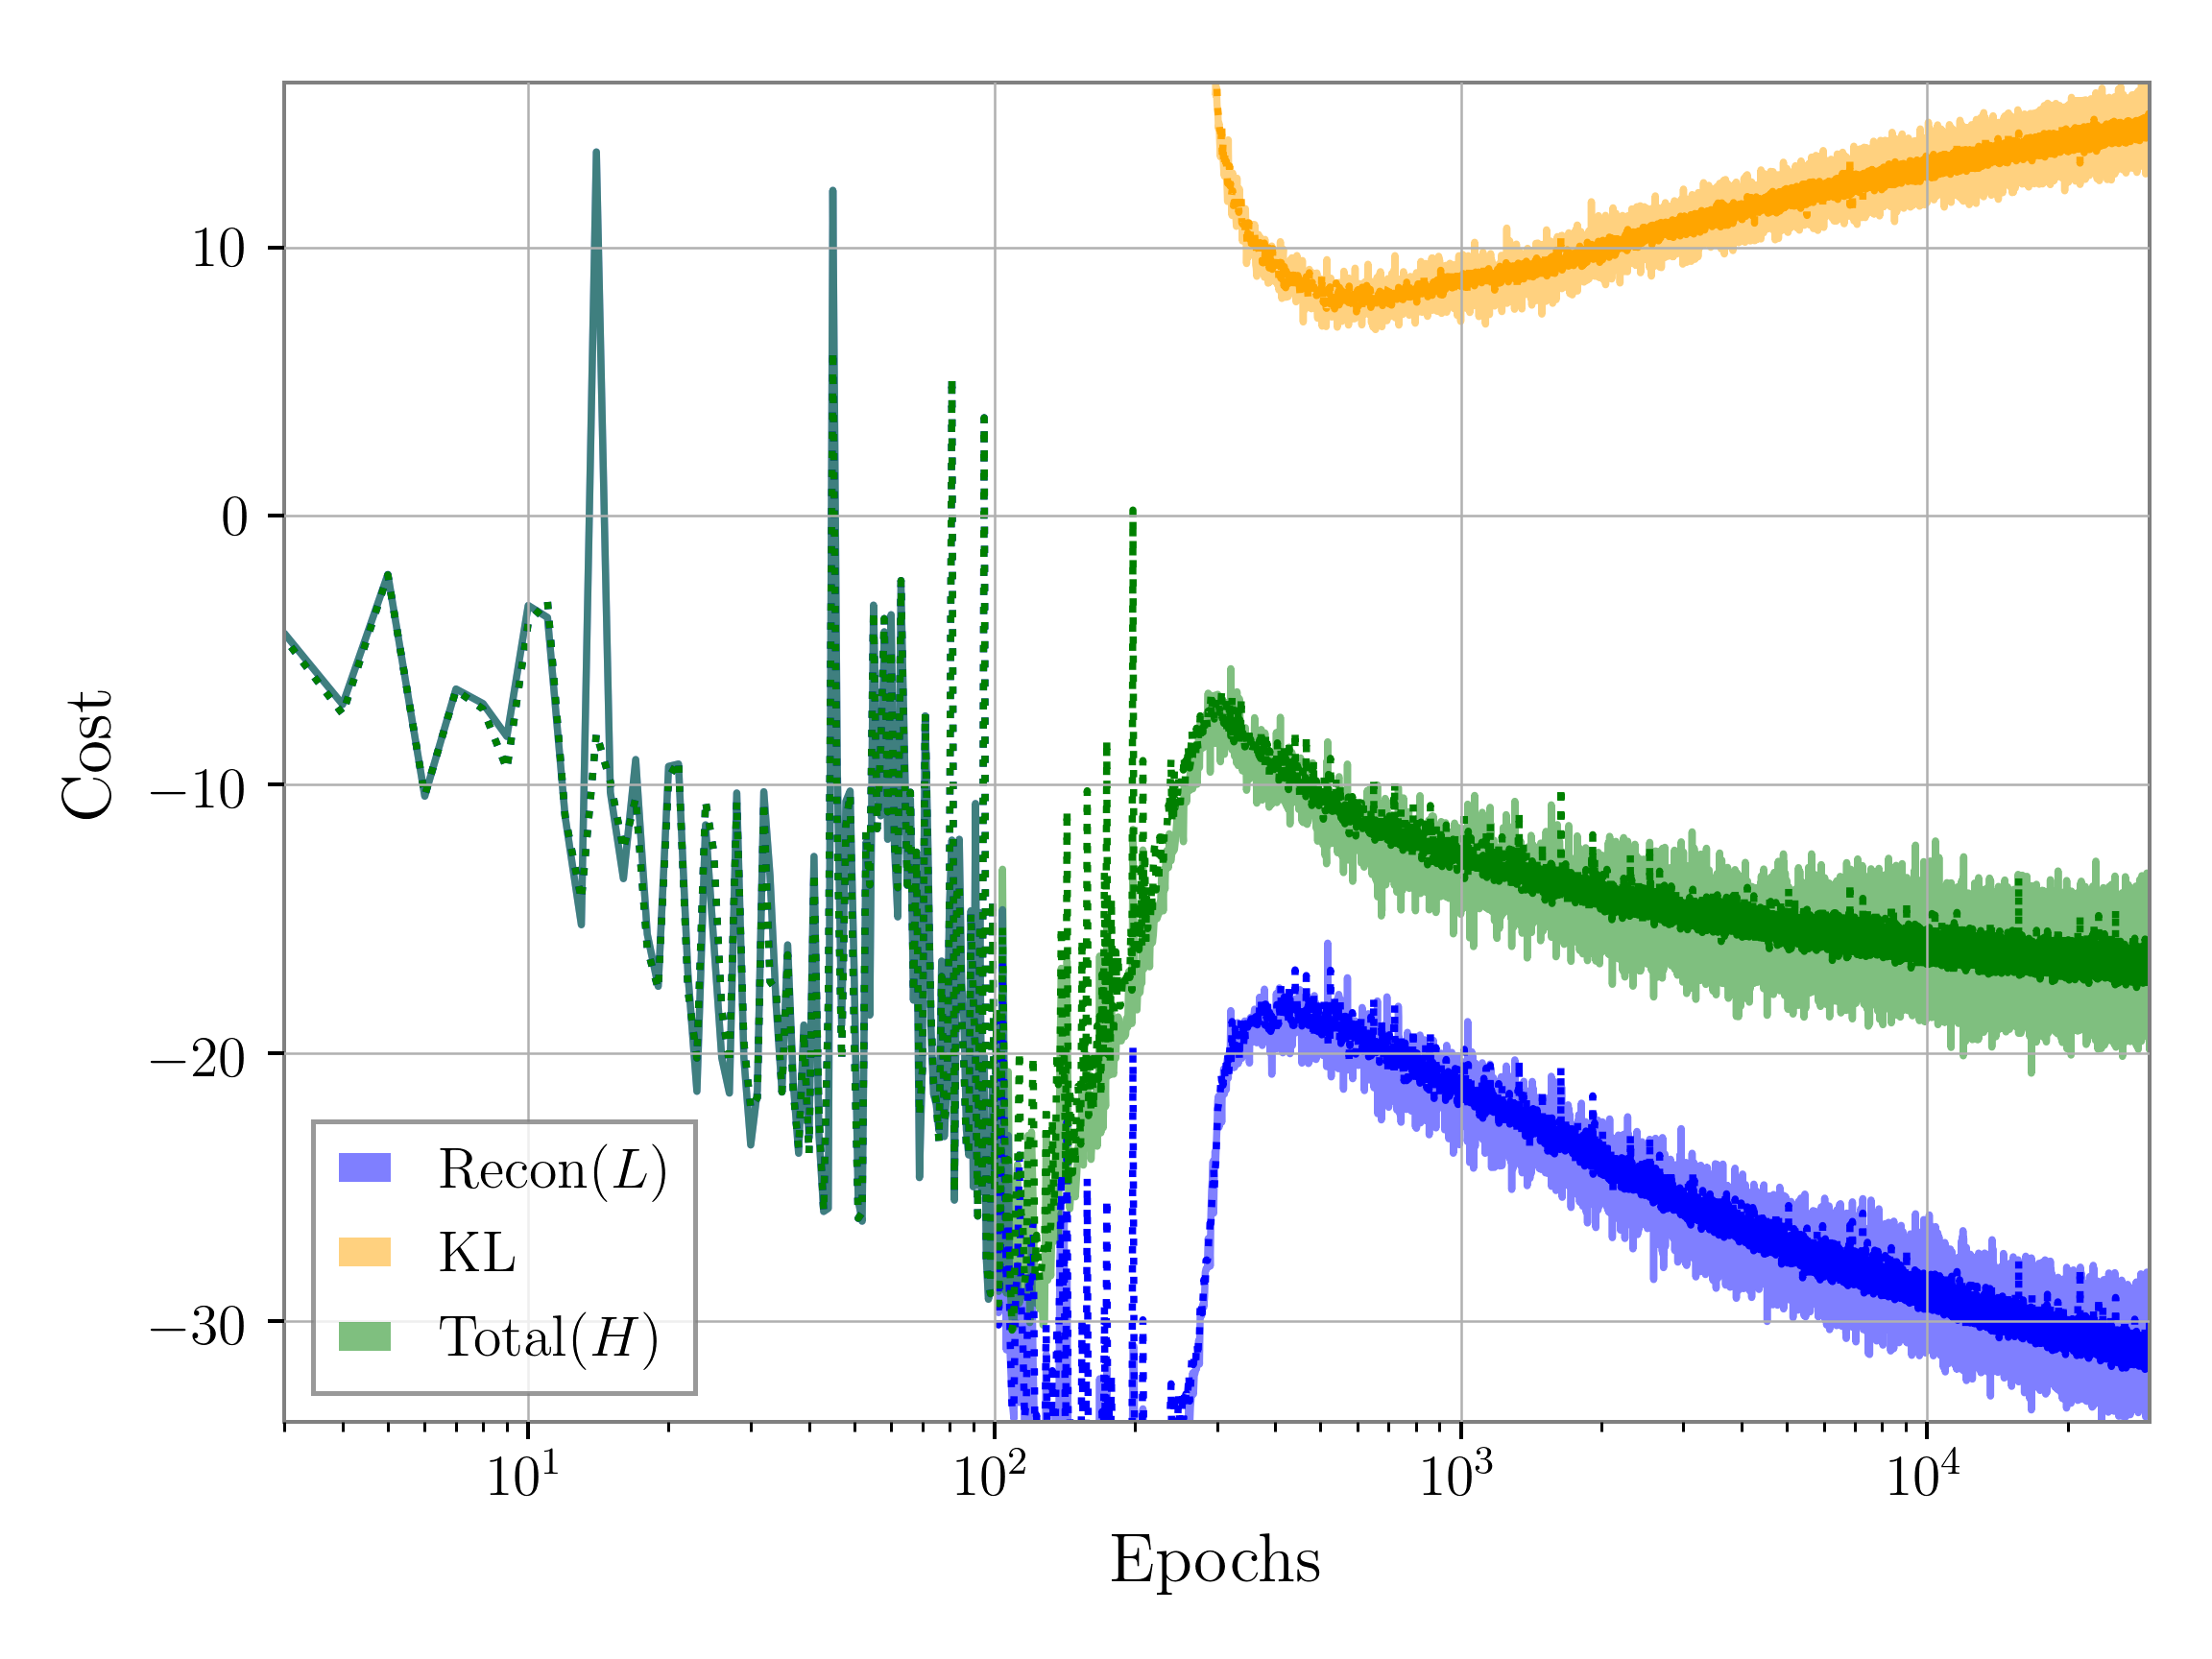
\includegraphics[width=\columnwidth]{inv_losses_log.png}
\caption{\label{fig:loss_log} The cost as a function of training epoch. 
We show the total cost function (green) together with its component parts: 
the \ac{KL}-divergence component (orange) and the reconstruction 
component (blue) which are simply summed to obtain the total. 
The dark curves correspond to the cost computed per epoch, 
defined as the network seeing $2\times10^{4}$ data samples, 
of training data and the lighter curves
represent the cost when computed on independent validation data. 
The close agreement between training and validation cost values 
indicates that the network is not overfitting to the training data. 
The change in behavior of the cost between $10^2$ and $3\times10^2$ 
epochs is a consequence of gradually introducing the \ac{KL} 
cost term contribution via an annealing process, described in 
Sec.~\ref{sec:training_procedure}.} 
\end{figure}



%%%%%%%%%%%%%%%%%%%%%%%%%%%%%%%%%%%%%%%%%%%%%%%%%%%%%%%%%%%%%%%%%%%%%%
\section{VItamin Network Design}\label{sec:network_design}
%
% Describe the specific network hyper-parameters
%

%
% Describe the specific network architecture design
%
The \ac{CVAE} network outlined in Fig.~\ref{fig:network_config} is 
constructed from the 3 separate neural networks modelling the encoder and 
decoder distributions $r_{\theta_1}$ and $r_{\theta_2}$ as well as 
the recognition function $q_{\phi}$. Each of these components is a 
deep convolutional network consisting of a series of 
one-dimensional convolutional layers followed by a series of 
fully-connected layers. The details of each network structure are 
given in Table~\ref{Tab:network_design} where we indicate the 
activations used. We arrived at this network design through a combination 
of trial and error and Bayesian optimisation using Gaussian
Processes~\cite{Siria2020.06.11.144253} (using the \texttt{scikit-optimize}
toolkit~\cite{scikit-learn}). After much testing, it turns out that 
our network chosen through trial and error was superior in performance 
to that of the Bayesian optimisation algorithm. 

%
% I feel the need, the need to clearly define our CVAE networks
%
\begin{table*}
\resizebox{14cm}{!}{
\begin{minipage}{\linewidth}
\centering
\caption{The \texttt{VItamin} network hyper-parameters. Dashed lines ``---'' indicate that 
convolutional layers are shared between all 3 networks. \hunter{could 
state total number of network hyperparameters.} }
\begin{tabular}[t]{l|ccc}
\toprule
\backslashbox{Layer}{Network} & $r_{\theta_1}(z|y)$ & $r_{\theta_2}(x|y,z)$ & $q_{\phi}(z|x,y)$ \\
\hline
%%%%%%%%%%%%%%%%%%%%%%%%%%%%%%%%
\multirow{2}{*}{Input $y$} & \multirow{2}{*}{[1024,3]\footnote{The shape of the
data [one-dimensional dataset length, No. channels].}} &
\multirow{2}{*}{[1024,3]} & \multirow{2}{*}{[1024,3]} \\
& & & \\
\hline
%%%%%%%%%%%%%%%%%%%%%%%%%%%%%%%%
\multirow{2}{*}{Layer 1} & conv(64,3,96)\footnote{one-dimensional
convolutional filter with arguments (filter size, No. channels, No. filters).} & --- & --- \\
& L2Reg(0.001)\footnote{L2 regularization funciton applied to the kernel weights 
matrix.} & --- & --- \\
& act\footnote{The activation function used.}=LeakyReLU & --- & --- \\
\hline
%%%%%%%%%%%%%%%%%%%%%%%%%%%%%%%%
\multirow{3}{*}{Layer 2} & conv(32,96,96) & --- &
--- \\
& stride(4)\footnote{Striding layer with arguments (stride
length).} & --- & --- \\
& L2Reg(0.001) & --- & --- \\
& act=LeakyReLU & --- & --- \\
\hline
%%%%%%%%%%%%%%%%%%%%%%%%%%%%%%%%
\multirow{2}{*}{Layer 3} & conv(32,96,96) & --- &
--- \\
& L2Reg(0.001) & --- & --- \\
& act=LeakyReLU & --- & --- \\
\hline
%%%%%%%%%%%%%%%%%%%%%%%%%%%%%%%%
\multirow{2}{*}{Layer 4} & conv(16,96,96) & --- &
--- \\
& stride(2) & --- & --- \\
& L2Reg(0.001) & --- & --- \\
& act=LeakyReLU & --- & --- \\
\hline
%%%%%%%%%%%%%%%%%%%%%%%%%%%%%%%%
\multirow{2}{*}{Layer 5} & conv(16,96,96) & --- &
--- \\
& L2Reg(0.001) & --- & --- \\
& act=LeakyReLU & --- & --- \\
\hline
%%%%%%%%%%%%%%%%%%%%%%%%%%%%%%%%
\multirow{2}{*}{Layer 6} & conv(16,96,96) & --- &
--- \\
& stride(2) & --- & --- \\
& L2Reg(0.001) & --- & --- \\
& act=LeakyReLU & --- & --- \\
\hline
%%%%%%%%%%%%%%%%%%%%%%%%%%%%%%%%%
\multirow{2}{*}{Input $z,x$} & \multirow{2}{*}{flatten\footnote{Take the multi-channel output of the previous layer and
reshape it into a one-dimensional vector.}$\rightarrow$[6144]} &
flatten$\rightarrow$[6144] & flatten$\rightarrow$[6144] \\
& & append\footnote{Append the argument to the current dataset.}($z$)$\rightarrow$[6159] & append($x$)$\rightarrow$[6159] \\
\hline
%%%%%%%%%%%%%%%%%%%%%%%%%%%%%%%%%
\multirow{3}{*}{Layer 7} & 
\multirow{3}{*}{
\begin{tabular}[t]{c}
FC(6159,4096)\footnote{Fully
connected layer with arguments (input size, output size).}\\
act=LeakyReLU \\
\end{tabular}
} & 
\multirow{3}{*}{
\begin{tabular}[t]{c}
FC(6159,4096) \\
act=LeakyReLU \\
\end{tabular}
} &
\multirow{3}{*}{
\begin{tabular}[t]{c}
FC(6159,4096) \\
act=LeakyReLU \\
\end{tabular}
} \\
& & & \\
& & & \\
\hline
%%%%%%%%%%%%%%%%%%%%%%%%%%%%%%%%%
\multirow{3}{*}{Layer 8} & 
\multirow{3}{*}{
\begin{tabular}[t]{c}
FC(4096,2048)\\
act=LeakyReLU \\
\end{tabular}
} & 
\multirow{3}{*}{
\begin{tabular}[t]{c}
FC(4096,2048) \\
act=LeakyReLU \\
\end{tabular}
} &
\multirow{3}{*}{
\begin{tabular}[t]{c}
FC(4096,2048) \\
act=LeakyReLU \\
\end{tabular}
} \\
& & & \\
& & & \\
\hline
%%%%%%%%%%%%%%%%%%%%%%%%%%%%%%%%%
\multirow{3}{*}{Layer 9} & 
\multirow{3}{*}{
\begin{tabular}[t]{c}
FC(2048,1024)\\
act=LeakyReLU \\
\end{tabular}
} & 
\multirow{3}{*}{
\begin{tabular}[t]{c}
FC(2048,1024)\\
act=LeakyReLU \\
\end{tabular}
} &
\multirow{3}{*}{
\begin{tabular}[t]{c}
FC(2048,1024) \\
act=LeakyReLU \\
\end{tabular}
} \\
& & & \\
& & & \\
\hline
%%%%%%%%%%%%%%%%%%%%%%%%%%%%%%%%%
\multirow{4}{*}{Layer 10} & 
\multirow{4}{*}{
\begin{tabular}[t]{c}
FC(1024,960) \\
act=None \\
output=$\mu_{r_1}$ \\
$\rightarrow$[15,32,2]\footnote{The $r_{\theta_1}$ output has size
[latent space dimension, No. modes, No. parameters defining each
component per dimension].} \\
\end{tabular}
} & \multirow{4}{*}{
\begin{tabular}[t]{c}
FC(1024,30) \\
act=(Sigmoid,-ReLU)\footnote{Different activations are used for different
parameters. For the scaled parameter means we use
sigmoids and for log-variances we use negative ReLU functions.} \\
output=$\mu_{r_2}$ \\
$\rightarrow$[19,2]\footnote{The $r_{\theta_2}$ output has size [physical space dimension+additional cyclic dimensions, No. parameters defining
the distribution per dimension].  The addtional cyclic dimensions account for the 2 parameters 
each cyclic parameter is represented by in the abstract 2D plane.} \\
\end{tabular}
} &
\multirow{4}{*}{
\begin{tabular}[t]{c}
FC(1024,30) \\
act=None \\
output=$\mu_{q}$ \\
$\rightarrow$[15,2]\footnote{The $q_{\phi}$ output has size [latent space
dimension, No. parameters defining the distribution per dimension].} \\
\end{tabular}
} \\
& & & \\
& & & \\
& & & \\
\botrule
\end{tabular}
%\end{tabularx}
\label{Tab:network_design}
\end{minipage}
}
\end{table*}  

%
% describe the r1 network
%
The $r_{\theta_1}$ network takes the input timeseries data $y$ in the 
form of multi-channel 1-dimensional vectors where channels represent 
different \ac{GW} detectors. After passing through a series 
of 1-dimensional convolutional and fully connected layers, the 
output then defines the parameters of a $n_z$-dimensional 
(diagonal covariance matrices) Gaussian mixture model in the latent space. 
We label these parameters as $\mu_{r_1}$ containing $n_z\times M$ means 
and log-covariances, where $M=32$ mixture component weights 
and $n_z = 15$. The motivation for using this mixture model 
representation comes from the multi-modal nature of \ac{GW} 
posterior distributions. The encoder network can use this 
flexibility to represent the $y$ timeseries data as belonging to 
multiple possible latent space regions.   

%
% describe the q network
% 
The recognition function network $q_{\phi}$ is very similar to 
the $r_{\theta_1}$ network with only 2 differences. The network 
takes as input the $y$ timeseries and the true signal parameters 
$x$, however, only the $y$ data is passed through the 
1-dimensional convolutional layers. Only after the final convolutional 
layer where the output is flattened is the $x$ data appended. It is 
then this compound timeseries data ``feature-space'' and true signal 
parameters that are processed using the remaining fully-connected layers. 
The second difference is that the output of the network defines 
a \emph{single-modal} (diagonal) $n_z$-dimensional Gaussian. We label 
these parameters as $\mu_{q}$ containing $n_z=15$ means and 
log-covariances. The rationale behind this choice is that since 
the $q_{\phi}$ distribution is conditional on the true signal parameters, 
there should be no ambiguity as to which mode in the latent 
space that a particular timeseries belongs to.      

%
% describe the r2 network (bespoke output distributions)
%
The decoder network $r_{\theta_2}$ is identical in structure to the 
$q_{\phi}$ network but with a difference in the form of their 
outputs and inputs. The $r_{\theta_2}$ network takes as input both 
latent space samples $z$ and timeseries $y$. The $r_{\theta_2}$ output 
represents the parameters ($\mu_{r_2}$) that govern an 
$n_x$-dimensional distribution in the physical parameter space 
where we have carefully chosen appropriate distributions for each 
of the physical parameters. For the  
luminosity distance, the binary 
inclination, the time of coalescence, and spin 
parameters $a_1,a_2,\Theta_1,\Theta_2$ we have adopted truncated 
Gaussian distributions where the truncation occurs at the predefined 
prior boundaries of the respective parameter space dimensions. For the 
component masses we had initially adopted conditional truncated Gaussians where 
the conditional aspect was to ensure that 
$m_{1}\geq m_{2}$\footnote{We note that 
this additional complication of requiring conditional 
decoder output distributions could have been avoided if a 
different mass parameterisation were chosen, e.g., total mass and 
symmetric mass ratio.}, but found that training duration increased significantly 
because of this choice. We also found that the network typically learned
this conditional boundary based on the training data alone anyways, so have now 
instead opted for using truncated Gaussian distributions alone for 
$m_1$ and $m_2$. 
Independent von Mises distributions are applied to 
phase, polarisation angle and spin parameters $\phi_{12},\phi_{jl}$ in 
order to capture the periodic nature of these parameters. We 
model all cyclic parameters as locations in an abstract 2D plane (Sec.~\ref{sec:vit_data_aug}) 
and apply an additional reprameterisation on $\phi_0$ and $\psi$
(Sec.~\ref{sec:phipsi_repar}). Finally, we 
use the von Mises-Fisher distribution to model the right ascension 
and declination (sky) parameters.
% Additional details to note ... 

~\chris{You have to opportunity to explain this all in more detail here, e.g., how the mode weights are all in log-space and un-normalised, how the FVM requires 3 input parameters (x,y,z on the unit sphere). You could even define the mathematical equations describing each of the output distributions.}    

%%%%%%%%%%%%%%%%%%%%%%%%%%%%%%%%%%%%%%%%%%%%%%%%%%%%%%%%%%%%%%%%%%%%%%%%%%%%%%
%%%%%%%%%%%%%%%%%%%%%%%%%%%%%%%%%%%%%%%%%%%%%%%%%%%%%%%%%%%%%%%%%%%%%%
\section{Training Procedure}\label{sec:training_procedure}
%
% Introduce the training process
%
Our cost function is composed of 3 probability distributions 
modelled by neural networks with well defined inputs and outputs 
where the mapping of those inputs to outputs is governed by the parameter sets
$\theta_{1},\theta_{2}$ and $\phi$. These parameters are the 
weights and biases of 3 neural networks acting as (variational) 
encoder, decoder, and encoder respectively, as well as the trainable 
parameters of the optimiser. To train such a network one must 
connect the inputs and outputs appropriately to compute the cost 
function $H$ (Eq.~\ref{eq:cost3}) and back-propagate cost 
function derivatives to update the network parameters. 

%
% Go through the training step by step
%
Training is performed via a series of steps illustrated schematically in Fig.~\ref{fig:network_config}. A batch of data composed of pairs of timeseries $y$ and their corresponding true \ac{GW} signal parameters $x$ are passed as input and the following steps are applied to each element of the batch.
%
\begin{enumerate}
%
\item The encoder $q_{\phi}$ takes both the timeseries $y$ and the true parameters $x$ defining the \ac{GW} signal. It then encodes these instances into parameters $\mu_{q}$ defining an uncorrelated (diagonal covariance matrix) $n_z$-dimensional Gaussian distribution in the latent space. 
%
\item The encoder $r_{\theta_1}$ is given only the timeseries data $y$ and encodes it into a set of variables $\mu_{r_1}$ defining a multi-component multivariate Gaussian mixture distribution in the latent space.
%
\item We then draw a sample from the distribution described by $\mu_{q}$ giving us a location $z_{q}$ within the latent space.
%
\item This sample, along with its corresponding $y$ data, are then passed as input to the decoder $r_{\theta_2}$. This decoder outputs $\mu_{\theta_2}$ comprising a set of parameters that define a distribution in the physical $x$ space. 
 %
\item The first term of the loss function, the reconstruction loss (defined as $L$ in Eq.~\ref{eq:cost3}), is then computed by evaluating the probability density defined by $\mu_{\theta_2}$ at the true $x$ training value (the average is then taken over the batch of input data). 
%
\item The second loss component, the \ac{KL}-divergence between the distributions $q_{\phi}(z|x,y)$ and $r_{\theta_1}(z|y)$ (described by the parameter sets $\mu_{q}$ and $\mu_{r_1}$), is given as 
%
\begin{align}\label{eq:klgauss}
\text{KL}\left[ q_{\phi}(z|x_{n},y_{n})||r_{\theta_{1}}(z|y_{n})\right] 
= q_{\phi}(z|x_n,y_n) \log\left(\frac{q_{\phi}(z|x_n,y_n)}{r_{\theta_1}(z|y_n)}\right) \nonumber
%\right|_{z\sim
%q_{\phi}(z|x_n,y_n)}\nonumber
\end{align}
%
where $z_q$ is the sample drawn from $q_{\phi}(z|x_n,y_n)$ in the first 
training stage. We use this single-sample Monte-Carlo integration 
approximation since the \ac{KL}-divergence between a single-component 
and a multi-component multivariate Gaussian distribution has no analytic 
solution (the average is then taken over the batch of input 
data, hence the index $n$). 
%
\item The 2 loss components are then summed according to 
Eq.~\ref{eq:cost3} and all trainable network parameters 
(defined by $\theta_1,\theta_2,\phi$) are updated based on 
the derivative of the cost function with respect to these parameters.
%
\end{enumerate}

%
% the ramp
%
A problematic aspect of training relates to the behaviour of the 
network during the initial stages of training. The network has a 
strong tendency to become trapped in local minima resulting in a 
decreasing cost component $L$ (the reconstruction cost) but a 
non-evolving \ac{KL}-divergence term that remains close to zero. To 
avoid this state we apply an annealing process in which the \ac{KL}-
divergence term is initially ignored but its contribution is then 
increased logarithmically from 0 to 1 between the epoch 
indices $10^2$--$3\times10^2$. This allows the $q_{\phi}$ encoder to 
learn the latent space representation of the data via the reconstruction 
cost before being required to simultaneously try to best match its 
distribution to that modelled by the $r_{\theta_1}$ encoder. In 
parallel with the gradual introduction of the \ac{KL} cost term, we 
also find that the stability of training is negatively affected by the
complexity of our tailored output decoder likelihood functions. To 
resolve this we apply the same annealing procedure over the same epoch 
range in transitioning between unbound Gaussian likelihoods on all 
physical parameters to the tailored likelihoods, where the boundaries 
of the Gaussian likelihoods are brought in from $-10$ to $0$ on the 
lower bound and $11$ to $1$ on the upper bound.

%
% Some practical aspects of the training
%
As is standard practice in \ac{ML} applications, the cost is 
computed over a batch of training samples and repeated for a 
pre-defined number of epochs. An epoch traditionally is 
defined as the point at which 
the network has been trained on a number of samples equivalent to the 
size of the entire training set. However, in this study we define an epoch 
as the network having been trained on a number of samples equivalent to 
$2\times10^4$. For our purposes, we found that $\sim 3 \times 10^4$ 
training epochs, a batch size of $1500$ training samples and a learning 
rate of $10^{-4}$ was sufficient. We used a total of $10^7$ training 
samples in order to adequately cover the \ac{BBH} parameter space. 
We additionally ensure that an (effectively) infinite number of 
noise realizations are employed by making
sure that every time a training sample is used it is given a unique 
noise realisation despite only having a finite number of 
waveforms. Every epoch we also randomly shuffle the phase, time of coalescence 
and distance parameters for all training samples loaded in disk. See
Sec.~\ref{sec:vit_data_aug} for further details on 
data augmentation techniques used in this chapter. 

%
% completion of training and hardware
%
Completion of training is determined by comparing output posteriors on 
test samples with those of \texttt{Bilby} iteratively during 
training. This comparison is done using standard figures of merit such as 
the \ac{PP}-plot \ac{JS}-divergence (see Figs.~\ref{fig:pp_plot} 
and \ref{fig:kl_results}). We also assess training completion based on 
whether the evolution of the cost function and its component parts
(Fig.~\ref{fig:loss_log}) have converged~\chris{this is a fuzzy issue based on my smoothed loss curves which indicate that we are far from converged. This links to the study that you are doing on the theoretical lower limit on the cost based on the dynesty likelihoods and evidence values which you can link to here.}. We use a single Nvidia Tesla V100 \acp{GPU} with $16/32$ Gb of RAM although consumer grade ``gaming" \ac{GPU} cards are equally fast for this application. 
We also state that the onboard RAM memory of the machine/cluster itself 
has implications for the batch size and consequently the speed and 
optimal learning rate to use.

%%%%%%%%%%%%%%%%%%%%%%%%%%%%%%%%%%%%%%%%%%%%%%%%%%%%%%%%%%%%%%%%%%%%%%
\section{Testing Procedure}
%
% Introduce the testing procedure
%
After training has completed and we wish to use the network for inference 
we follow the procedure described in the right hand panel 
of Fig.~\ref{fig:network_config}. Given a new $y$ data sample 
(not taken from the training set) we simply input this into the trained 
encoder $r_{\theta_1}$ from which we obtain a single value of 
$\mu_{r_1}$ describing a distribution (conditional on the data $y$) 
in the latent space. We then repeat the following steps:

%
% Go through the testing step by step
%
\begin{enumerate}
%
\item We randomly draw a latent space sample $z_{r_1}$ 
from the latent space distribution defined by $\mu_{r_1}$.
%
\item The $z_{r_1}$ sample and the corresponding original $y$ 
data are fed as input to our pre-trained decoder network 
$r_{\theta_2}$. The decoder network returns a set of 
parameters $\mu_{r_2}$ which describe a multivariate 
distribution in the physical parameter space.
%
\item We then draw a random $x$ realisation from that distribution.
%
\end{enumerate}
%

%
% Final testing thoughts
%
A comprehensive representation in the form of samples drawn from the 
entire joint posterior distribution can then be obtained by 
simply repeating this procedure and hence sampling from our 
latent model $r_{\theta}(x|y)$ (see Eq.~\ref{eq:latent_model}).
We also note that some physical parameters are in-fact reparameterised in the 
neural network model (i.e. all cyclic parameters, $\phi_0$, $\psi$, and  
$\alpha$) and must then be converted back to their original 
parameterisation immediately 
following step 3 above. See Sec.~\ref{sec:vit_data_aug} for further details 
regarding how this is done.

%%%%%%%%%%%%%%%%%%%%%%%%%%%%%%%%%%%%%%%%%%%%%%%%%%%%%%%%%%%%%%%%%%%%%%%%%%%%%%
%%%%%%%%%%%%%%%%%%%%%%%%%%%%%%%%%%%%%%%%%%%%%%%%%%%%%%%%%%%%%%%%%%%%%%%%%%%%%%
\section{Primary VItamin Results}
%
We present results on $250$ multi-detector \ac{GW} test 
\ac{BBH} waveforms in simulated advanced detector 
noise~\cite{aligo_noisecurves} from the LIGO Hanford, 
Livingston and Virgo detectors. We compare between
variants of the existing Bayesian approaches and our 
\ac{CVAE} implementation which we call \texttt{VItamin}. 
Posteriors produced by the \texttt{Bilby} inference 
library~\cite{1811.02042} are used as a benchmark in order to 
assess the efficiency and quality of our machine learning approach 
with the existing methods for posterior sampling.

%
% describe the Bilby analysis 
%
For the benchmark analysis we assume that 14 parameters are
unknown: the component masses
$m_1,m_2$, the luminosity distance $d_{\text{L}}$, the sky position
$\alpha,\delta$, the binary inclination $\Theta_{jn}$, the \ac{GW} polarisation
angle ${\psi}$, the time of coalescence $t_{0}$, and the spin parameters $a_1,a_2,
\Theta_1,\Theta_2,\phi_{12},\phi_{jl}$.  We do not include phase $\phi_0$ in our 
results 
because we apply phase marginalisation to all Bayesian samplers since 
this 
improves overall stability and runtime~\cite{1811.02042}. For each parameter we use a uniform prior 
with the exception of the declination, inclination, and tilt angle 
parameters for 
which we use priors uniform in $\cos\delta$, $\sin\Theta_{jn}$, $\sin\Theta_1$, 
and $\sin\Theta_2$ respectively. We also use a conditional mass prior, 
such that $m_2$ is constrained to be $m_2 < m_1$. The corresponding 
prior ranges are defined in Table~\ref{tab:prior_ranges} and 
result in a training set \ac{SNR} distribution that has a median value of 
$\text{SNR}\approx 9$ and ranging between 0 and 
85 (see Fig.~\ref{fig:VItamin_TrainingSet_SNR_Dist}). We use a 
sampling frequency of $1024$~Hz, a timeseries duration of 1~s, and 
the waveform model used is \texttt{IMRPhenomPv2}~\cite{1809.10113} with 
a minimum cutoff frequency of $20$Hz. For each input test 
waveform we run the benchmark analysis using multiple 
sampling algorithms (\texttt{ptemcee},\texttt{Dynesty},\texttt{emcee},
\texttt{CPnest}) available within \texttt{Bilby}. For each run and 
sampler we extract $\mathcal{O}(8000)$ samples from the posterior on the 
14 physical parameters.

%
% discussion on sampler settings
%
With regards to the parameters choices in Table~\ref{Tab:sampler_params}, 
after having discussed with experts in the Bayesian sampler community, 
it is evident that Bayesian samplers are certainly not guaranteed 
to converge to the same results. Full convergence in many cases may 
require much fine tuning over many iterations for each individual run. 
Although we do not fine tune Bayesian benchmark samplers for each 
sampler and each individual test case, we do use settings which 
have been recommended to us by \texttt{bilby} developers and outside experts 
for each respective Bayesian sampler. Both the \texttt{Dynesty} and 
\texttt{CPNest} 
samplers have a tolerance threshold (change in the log evidence 
from one proposal to the next) which guarantees a certain level of 
convergence. We use the recommended tolerance level of 0.1 for 
both nested samplers. For the \ac{MCMC} samplers, \texttt{emcee} 
performs poorly, 
but is known to have difficulties with convergence within the 
community. There are a handful of \texttt{ptemcee} test cases 
(~5 of the 250) which show some minor indication of incomplete 
convergence, but after careful review we have determined that a 
lengthier burn-in period does not significantly improve the 
resulting posteriors.

%
% I feel the need, the need for clearly outlining the bilby parameter choices
%
\begin{table*}
\centering
\caption[Benchmark sampler configuration parameters.]{Benchmark sampler configuration parameters. Values were chosen based on a combination of their recommended default parameters~\cite{1811.02042} and private communication with the \texttt{Bilby} development team.}
\begin{minipage}{\linewidth}
\begin{tabular}[t]{lc}
\toprule
sampler & parameters \\
\hline
\texttt{Dynesty}~\cite{dynesty} & $\begin{array}{c} \text{live-points} =1000,\, \text{dlogz} =0.1,\, \text{nact} =50,\,  \text{npool} =8,\, \\ \text{bound} = \text{None},\, \text{sample} = \text{uniform} \end{array}$\\
\hline 
%\texttt{ptemcee}~\cite{ptemcee} & $\begin{array}{c}\text{walkers}=200\,
%\text{temperatures}=20\,
%\\ \text{nsamples}=10000\, \text{threads}=10\end{array}$ \\
\texttt{ptemcee}~\cite{ptemcee} & $\begin{array}{c}\text{walkers}=200,\, 
\text{temperatures}=20,\, \text{burn}\_\text{in}\_\text{nact}=50,\, \\ \text{thin}\_\text{by}\_\text{nact}=0.5,\, 
\text{nsamples}=10000,\, \text{threads}=10,\, \\ \text{autocorr}\_\text{tol}=50,\, 
\text{autocorr}\_\text{c} \text{safety}=1,\, \text{autocorr}\_\text{tau}=1,\, \\ 
\text{gradient}\_\text{tau}=0.1,\, 
\text{gradient}\_\text{mean}\_\text{log}\_\text{posterior}=0.1,\, \\ \text{Q}\_\text{tol}=1.01,\, 
\text{min}\_\text{tau}=1,\, \text{threads}=1,\, \end{array}$ \\
\hline
\texttt{CPNest}~\cite{cpnest} & $\begin{array}{c} \text{live-points} =2048,\, \text{maxmcmc} =1000, \, \text{nthreads} = 1,\, \\
\text{seed} = 1994,\, \text{dlogz} =0.1 \end{array}$ \\
\hline
\texttt{emcee}~\cite{emcee} & $\begin{array}{c} \text{nwalkers} =250,\, \text{nsteps} =14000,\, \text{nburn}=4000,\, \text{a} = 1.4,\, \\
\text{burn}\_\text{in}\_\text{fraction}=0.25,\, \text{burn}\_\text{in}\_\text{act}\_=3 \end{array}$ \\
\botrule
\end{tabular}
\label{Tab:sampler_params}
\end{minipage}
\end{table*}

%
% Priors
%
\begin{table}
\centering
\caption{The prior boundaries used on the \ac{BBH} signal parameters for the benchmark and the \ac{CVAE} analyses. We note that the polarisation angle and phase are represented in the 2D plane through a reprameterisation given in (Sec. ~\ref{sec:phipsi_repar}).}
\begin{minipage}{\linewidth}
\begin{center}
\begin{tabular}[t]{lccccc}
\toprule
Parameter name & symbol & min & max & units & prior function \\
\hline
mass 1 & $m_1$ & 35 & 80 & solar masses & Uniform \\
mass 2 & $m_2$\footnote{Additionally $m_2$ is constrained such that
$m_{2}<m_{1}$.} & 35 & 80 & solar masses & Uniform \\
luminosity distance & $d_{\text{L}}$ & 1 & 3 & Gpc & Uniform \\
time of coalescence & $t_{0}$ & 0.65 & 0.85 & s & Uniform \\
phase at coalescence & $\phi_{0}$ & 0 & $2\pi$ & radians & Uniform~\footnote{Phase 
has a periodic boundary condition.} \\
right ascension & $\alpha$ & 0 & $2\pi$ & radians & Uniform~\footnote{Right ascension 
has a periodic boundary condition.} \\
declination & $\delta$ & $-\pi/2$ & $\pi/2$ & radians & Cosine \\
inclination & $\iota$ & 0 & $\pi$ & radians & Sine \\
polarisation & $\psi$ & 0 & $\pi$ & radians & Uniform~\footnote{Polarisation 
has a periodic boundary condition.} \\
spin magnitude 1 & $a_1$ & 0 & 0.8 & - & Uniform \\
spin magnitude 2 & $a_2$ & 0 & 0.8 & - & Uniform \\
tilt angle 1 & $\Theta_1$ & 0 & $\pi$ & radians & Sine \\
tilt angle 2 & $\Theta_2$ & 0 & $\pi$ & radians & Sine \\
azimuthal angle & $\phi_{12}$ & 0 & $2\pi$ & radians & Uniform~\footnote{Azimuthal angle  
has a periodic boundary condition.} \\
azimuthal position & $\phi_{jl}$ & 0 & $2\pi$ & radians & Uniform~\footnote{Azimuthal position  
has a periodic boundary condition.} \\
\hline
%spins & - & \multicolumn{2}{c}{0} & - \\
epoch & \multicolumn{3}{c}{1126259642} & GPS time & - \\
detector network & \multicolumn{3}{c}{LIGO H1,L1, \& Virgo V1} & - & - \\
\botrule
\end{tabular}
\end{center}
\label{tab:prior_ranges}
\end{minipage}
\end{table}

\begin{figure}
    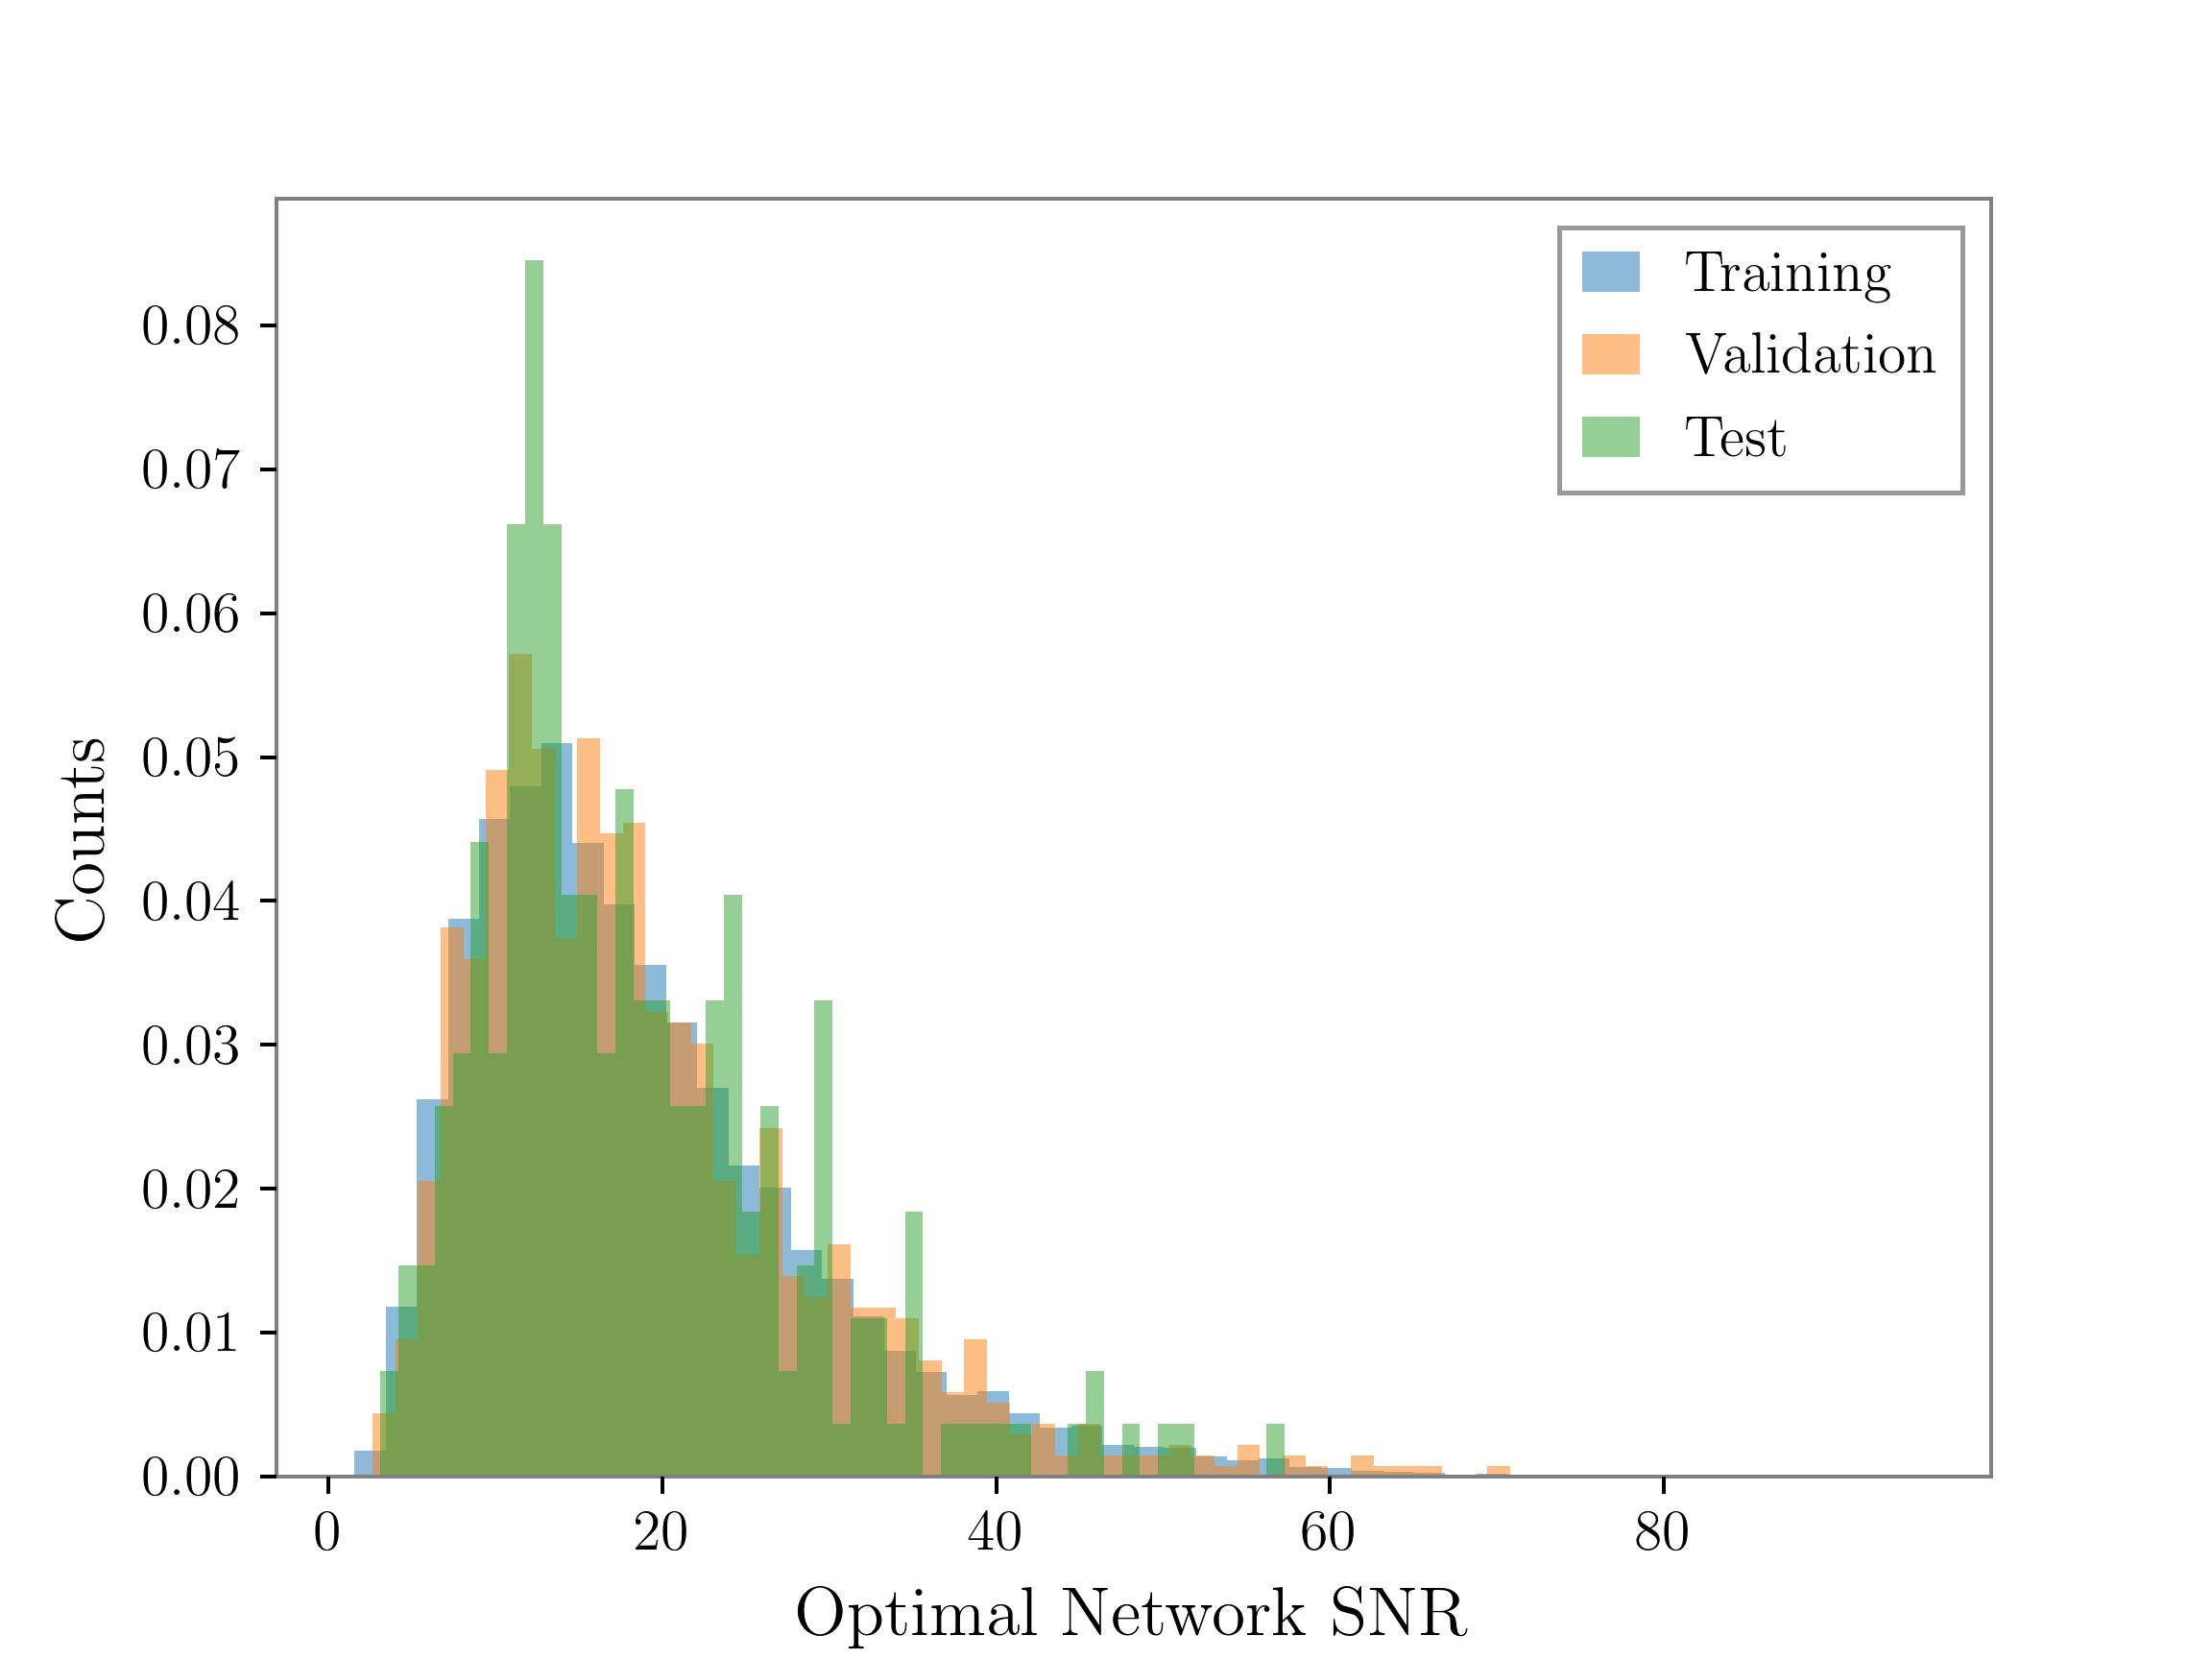
\includegraphics{figures/TrainingSetSNR_distribution.png}
    \caption[VItamin signal-to-noise ratio training, validation and testing set distributions.]{\label{fig:VItamin_TrainingSet_SNR_Dist} We show here a histogram of the optimal network \ac{SNR} values of the \texttt{VItamin} training, validation and testing sets. The mode for all 
    plotted distributions occurs at an \ac{SNR} value of $\sim8$ which drops off quickly to zero on the left-hand side. There is a tail on the right-hand side which drops off more gradually up to a maximum \ac{SNR} value of $\sim 85$ 
    for the training set, $\sim 70$ for the validation set and $\sim 57$ 
    for the testing set. The peak location and general distribution of the \ac{SNR} values is heavily dependent on both the chosen source parameter 
    priors (Tab.~\ref{tab:prior_ranges}) and the \ac{PSD}.}
\end{figure}

%
% the VItamin process
%
The \texttt{VItamin} training process uses as input 
$10^{7}$ whitened waveforms corresponding to parameters drawn 
from the same priors as assumed for the benchmark analysis. The 
waveforms are also of identical duration, sampling frequency, and 
use the same waveform model as in the benchmark analysis. 
The signals are whitened\footnote{The whitening is used 
primarily to scale the input to a magnitude range more suitable to 
neural networks. The \emph{true} \ac{PSD} does not have to be used for 
whitening, but training data and test data must be contain 
signals that have been whitened by the same \ac{PSD}.} using the same 
advanced detector \acp{PSD}~\cite{aligo_noisecurves} as assumed 
in the benchmark analysis. When each whitened waveform is 
placed within a training batch it is given a unique detector 
Gaussian noise realisation (after signal whitening this is simply 
zero mean, unit variance Gaussian noise). See Sec.~\ref{sec:vit_data_aug} 
for further data augmentation details. The \texttt{VItamin} posterior 
results are produced by passing each of our $250$ whitened noisy 
testing set of \ac{GW} waveforms as input into the testing path of 
the pre-trained \ac{CVAE} (Fig.~\ref{fig:network_config}). For each 
input waveform we sample until we have generated $8000$ posterior samples 
on 15 physical parameters 
$x=(m_1,m_2,d_{\text{L}},t_{0},\Theta_{jn},a_1,a_2,\Theta_1,
\Theta_2,\psi, \phi_0, \phi_{12},\phi_{jl},\alpha,\delta)$. We also note
that parameters (such as $\phi_0$) can (if desired) be 
marginalised out within the \ac{CVAE} procedure itself, rather than 
after training by choosing only to output a subset of the 
source parameter space in the final layer of the decoder network. When 
performing comparisons between the \texttt{VItamin} approach and other 
bilby samplers, we only compare using 14 parameters (i.e. excluding 
$\phi_0$) since we apply phase marginalisation to the bilby samplers when 
generating benchmark Bayesian test case posteriors. 

%
% Corner plot results
%
\begin{figure*}
    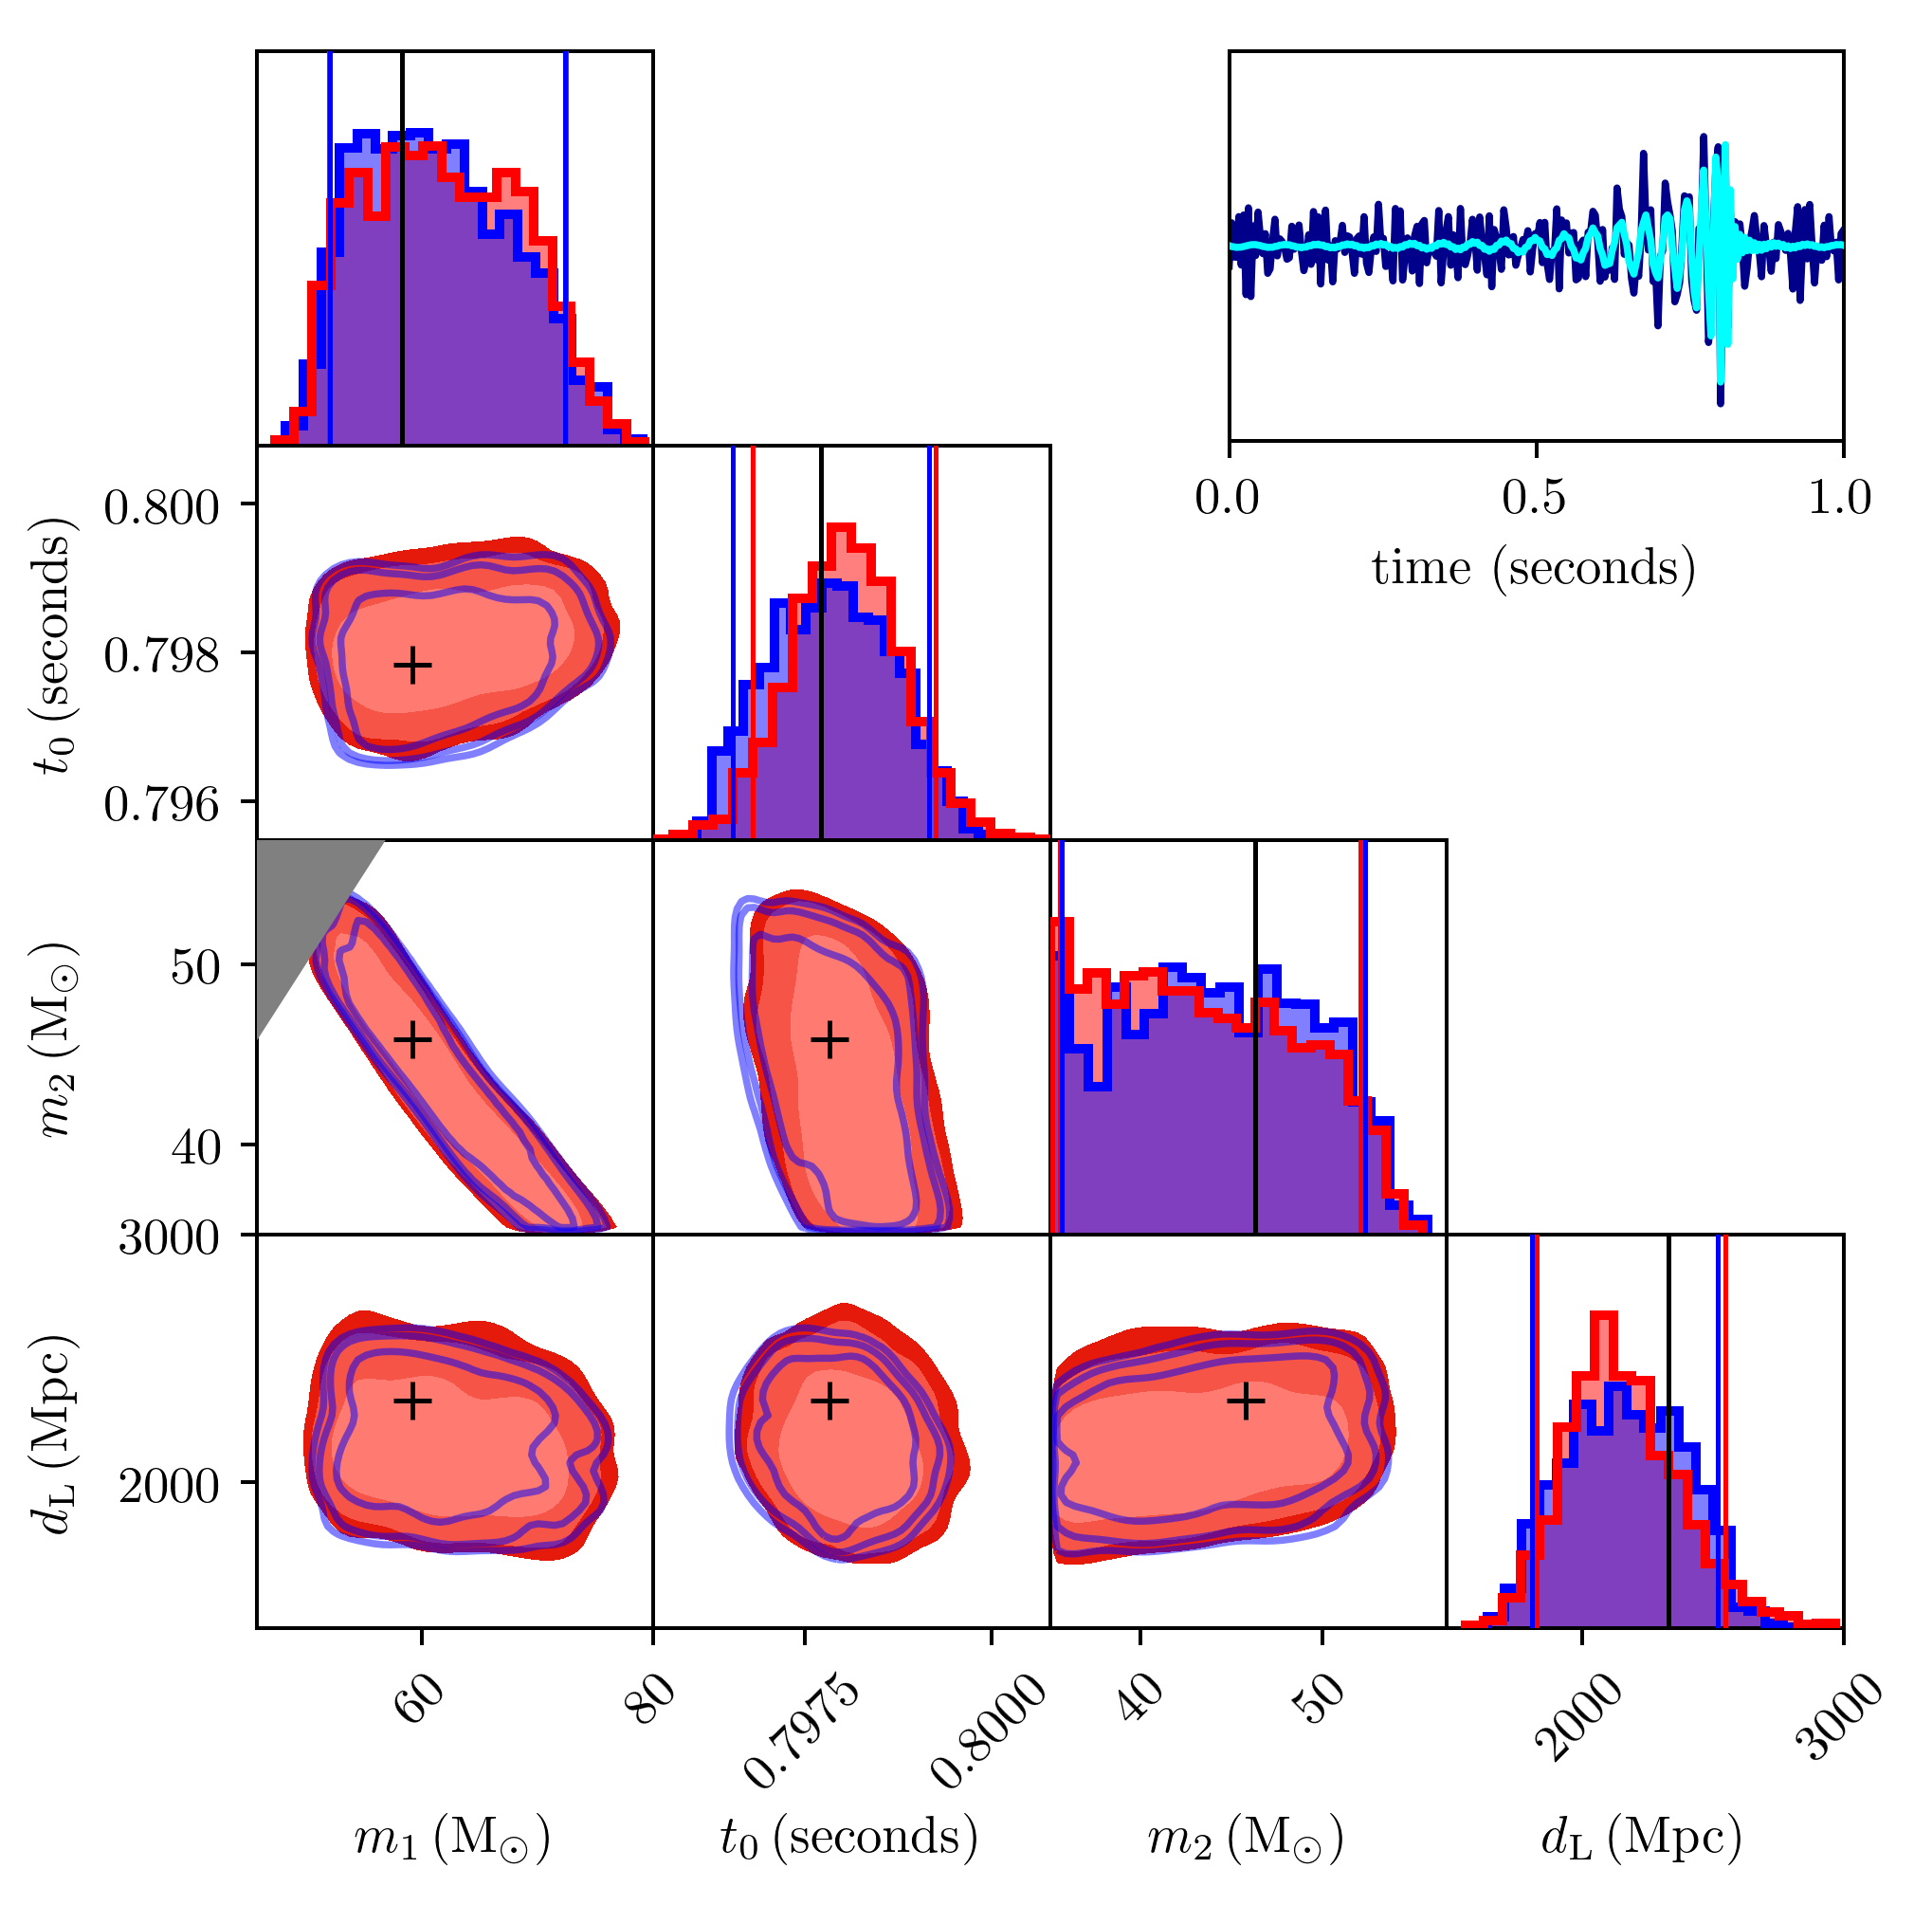
\includegraphics[width=\textwidth]{corner_testcase0.png}
    \caption[Corner plot showing 1 and 2-dimensional
    marginalised posterior distributions on the \ac{GW} parameters for 
    one example test dataset.]{\label{fig:corner_plot} Corner plot showing 
    1 and 2-dimensional marginalised posterior distributions on the 
    \ac{GW} parameters for one example test dataset. Red contours 
    represent the two-dimensional joint posteriors obtained from 
    \texttt{VItamin} and blue and green contours are the corresponding 
    posteriors output from our benchmark analyses 
    (using the \texttt{Dynesty} and \texttt{ptemcee} samplers 
    within \texttt{Bilby}). In each case, the contour boundaries enclose 
    $68,90$ and $95\%$ probability. 1 dimensional histograms of the 
    posterior distribution for each parameter from both methods are 
    plotted along the diagonal. Orange vertical and horizontal lines 
    denote the true parameter values of the simulated 
    signal. Vertical 
    dashed lines in the 1 dimensional plots are representative of the $5\%$ and 
    $95\%$ symmetric confidence bounds of the 3 sampler 1 dimensional posteriors.
    At the top right of the figure we include a Mollweide projection of 
    the sky location posteriors from all three analyses. All results 
    presented in this chapter correspond to a three-detector configuration 
    but for clarity we only plot the H1 whitened noisy timeseries $y$ and 
    the noise-free whitened signal (in blue and cyan respectively) to the 
    right of the figure. The test signal was simulated with an 
    optimal multi-detector signal-to-noise ratio of 14.3.~\chris{Try to make better use of the space - maybe increase the sky plot size and the timeseries plot. Th timeseries plot sould hav ethe legend removed and there is an argumnet for *all* fonts to be made larger for easier reading.}} 
\end{figure*}

%
% discuss the corner plot results
%
We can immediately illustrate the accuracy of our machine learning predictions
by directly plotting 2- and 1-dimensional marginalised posteriors generated
using the output samples from our \texttt{VItamin} and \texttt{Bilby}
approaches superimposed on each other. We show this for one example test
dataset in Fig.~\ref{fig:corner_plot} where strong agreement between the
\texttt{Bilby} sampler \texttt{Dynesty} in blue,  and the
\ac{CVAE} (red) is clear. It is also evident that whilst we refer to the
\texttt{Bilby} sampler results as benchmark cases, different existing samplers
do not perfectly agree with each other (i.e. \texttt{ptemcee} in green) despite using 
expert recommended sampler settings shown in Tab.~\ref{Tab:sampler_params}.  
For each of our 250 test cases we see
reasonable levels of agreement between pairs of benchmark samplers \emph{and}
between any benchmark sampler and our \ac{CVAE} results. 

%
% mention the p-p plot and KL distribution results
%
Figures~\ref{fig:pp_plot} and \ref{fig:kl_results}
show the results of multiple statistical 
tests (the \ac{PP} plot test and \ac{JS}-divergence tests) 
performed on the entire test dataset and between all samplers 
(\texttt{Dynesty}, \texttt{ptemcee}, \texttt{CPNest}, \texttt{emcee}, 
and \texttt{VItamin}). In
both tests the quality of the \texttt{VItamin} results are
 reasonably consistent with the
benchmark samplers
. 
% pp plot
A standard test used within the \ac{GW} parameter estimation community 
is the production of so-called \ac{PP} plots which we show for our 
analysis and the benchmark comparisons in Fig.~\ref{fig:pp_plot}. The plot 
is constructed by computing a cumulative probability for each 
1-dimensional marginalised test posterior evaluated at the true simulation parameter value (the fraction of posterior samples $\leq$ the simulation value). We then plot the cumulative distribution of these values~\cite{1409.7215}. Curves consistent with the black dashed diagonal line indicate that the 1-dimensional Bayesian probability distributions are consistent with the frequentist interpretation - that the truth will lie within an interval containing $X\%$ of the posterior probability with a frequency of $X\%$ of the time. It is clear to see that results obtained using \texttt{VItamin} show deviations from the diagonal that are entirely consistent with those observed in all benchmark samplers. The $p$-value has also been calculated for each sampler and each parameter under the null-hypothesis that they are consistent with the diagonal. These results show that for at least 1 parameter, emcee shows inconsistency with the modal at the 0.4\% level. \texttt{Dynesty} has a worst case that is consistent only at the 0.7\% level.  All other samplers (including \texttt{VItamin}) show consistency at $>0.4\%$ in the worst case.
What these \ac{PP} plot results show is that the posteriors produced 
by \texttt{VItamin}, whilst perhaps not optimal, are still trustworthy and are unbiased 
in their estimation.~\hunter{Is this enough of an explanation for the pp plot meaning?}
~\chris{Also, at some point, state what a pp plot actually means - why the Bayesian-Frequentist comparison is important.} 
~\chris{use the final p-values output from the code to back this up. 
Important results shouldn't only appear in figure captions. You actually 
give the best and worst p-values for each sampler but bilby should 
also output the overall p-value combining all parameters for a 
given sampler. It would be worth quoting those numbers}

%
% P-P plot
%
\begin{figure}
    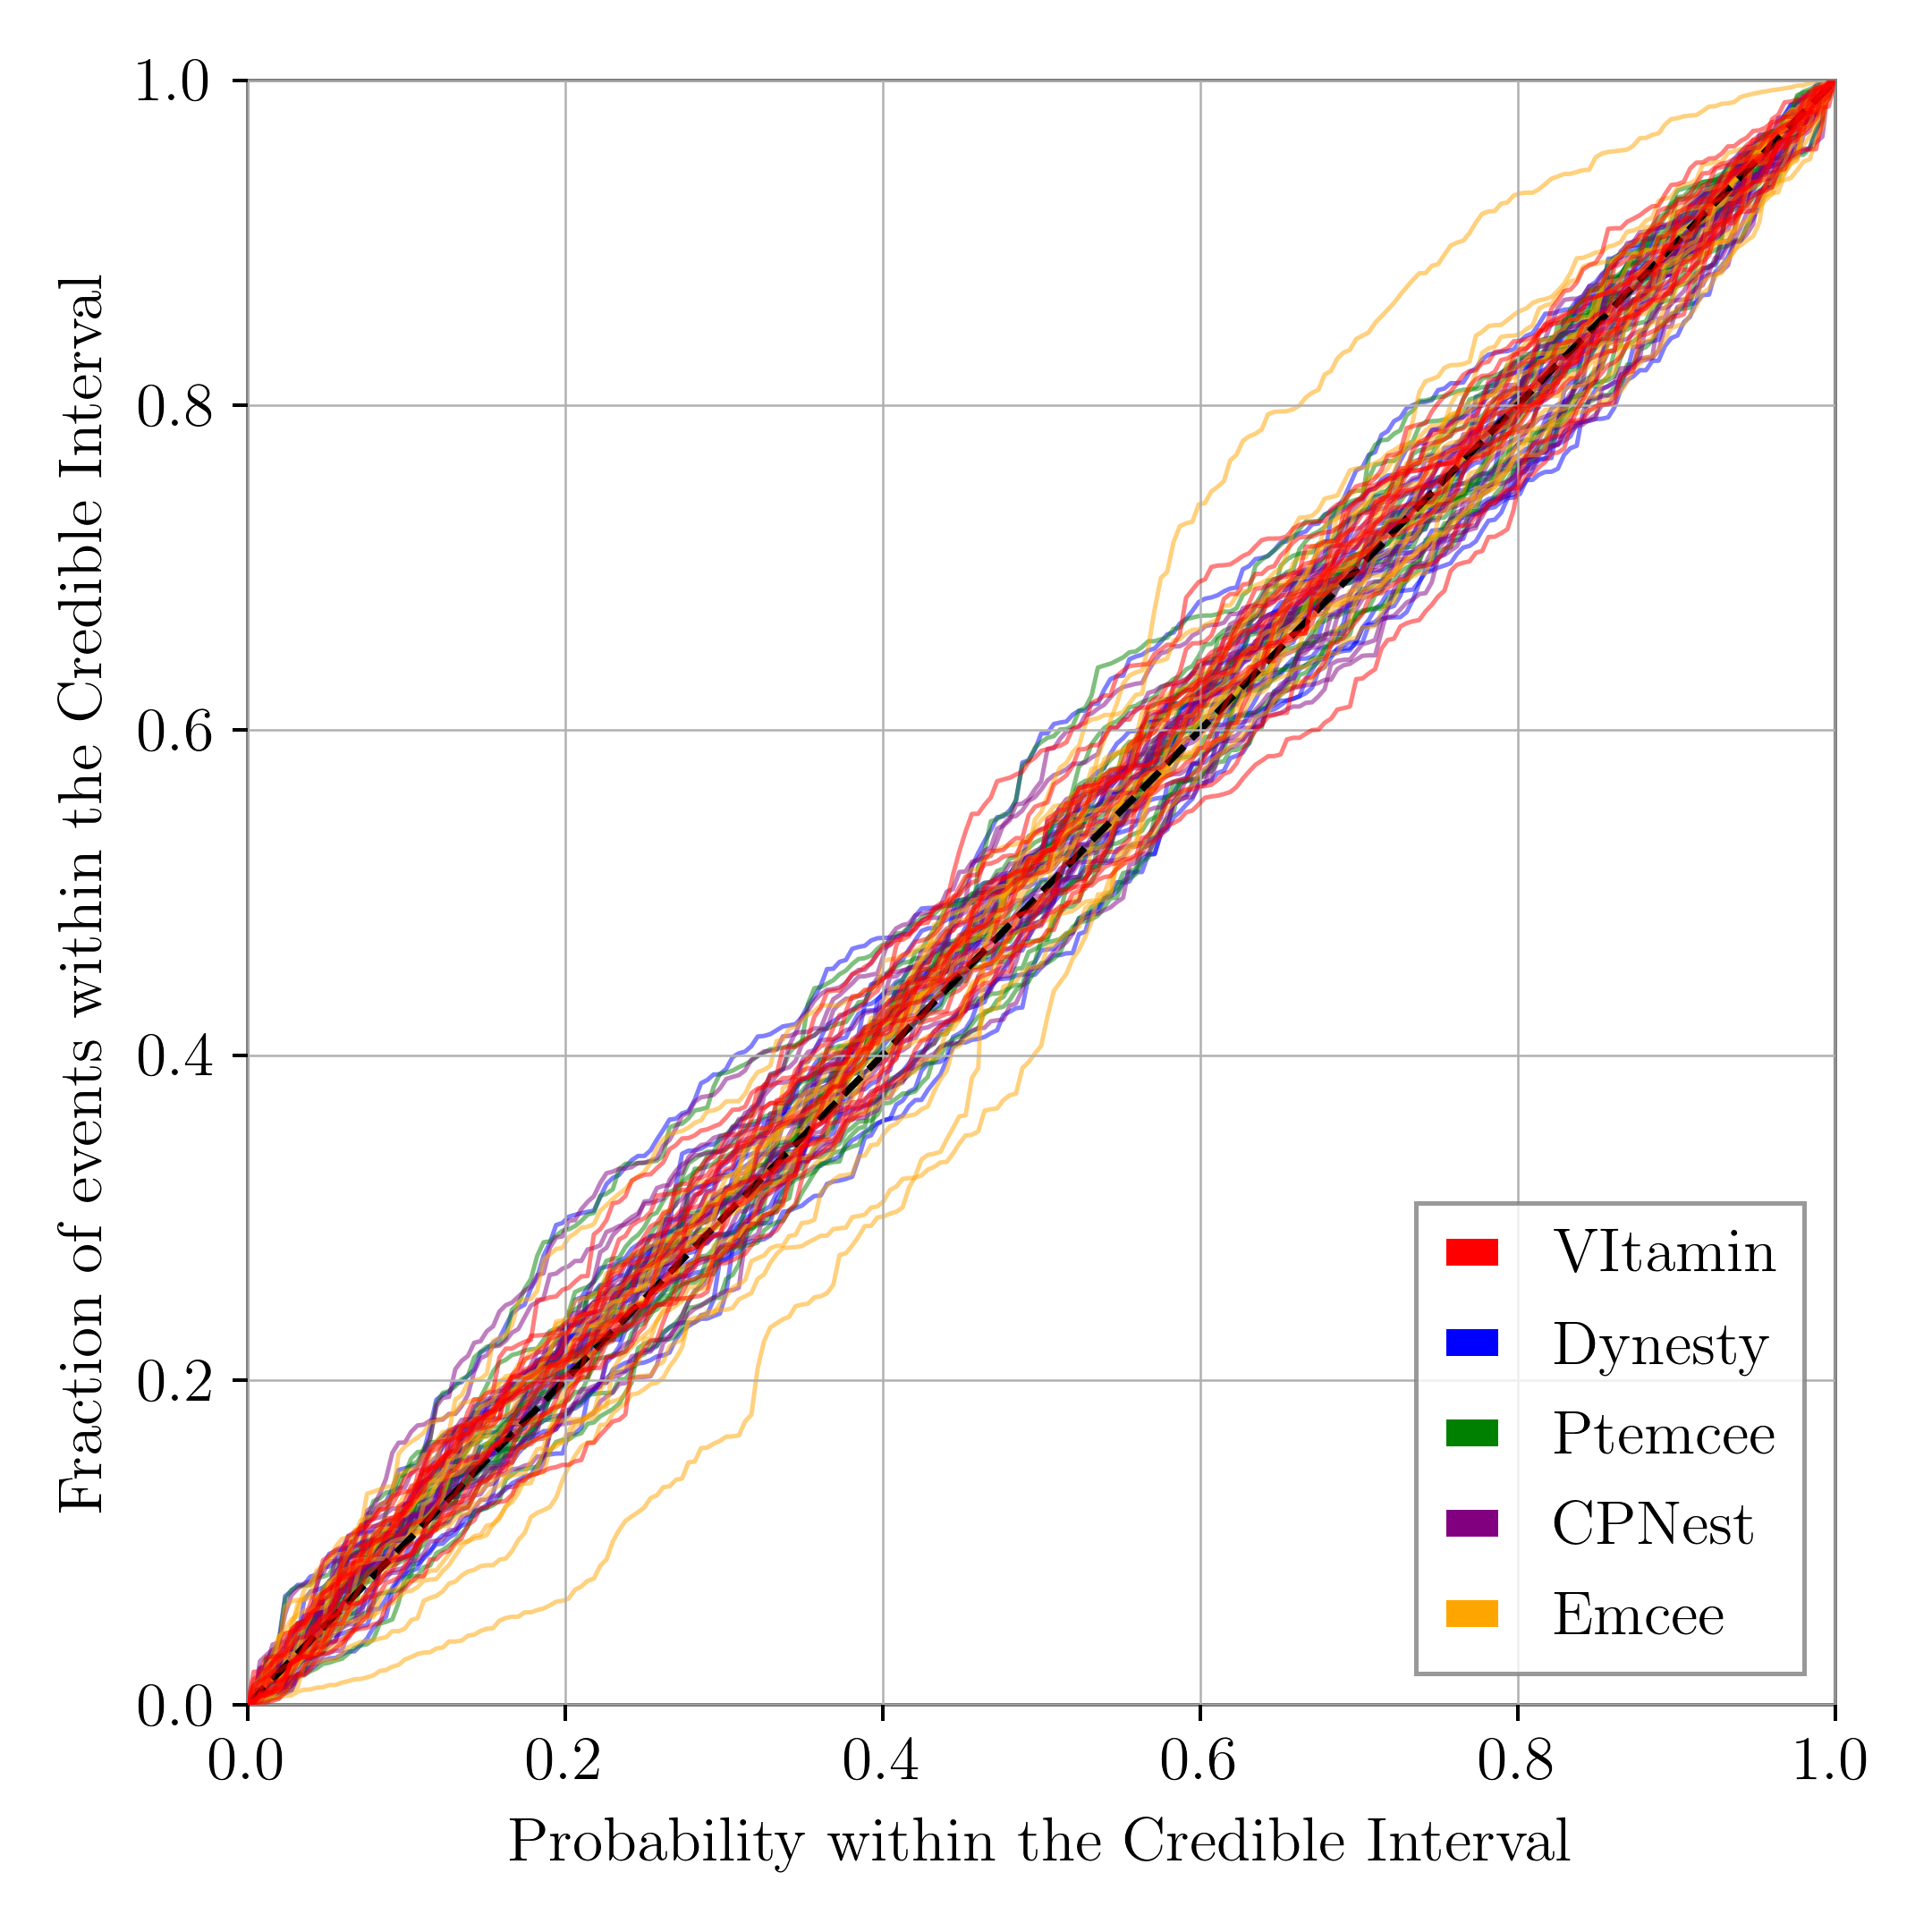
\includegraphics[width=\columnwidth]{latest_pp_plot.png}
    \caption[One-dimensional \ac{PP} plots for each parameter and for each benchmark sampler and \texttt{VItamin}.]{\label{fig:pp_plot}~\chris{You might consider using 4 panels in the thesis to better separate the curves from the different samplers. It might then warrant adding the grey error regions?} One-dimensional \ac{PP} plots for each parameter and for each benchmark sampler and \texttt{VItamin}. The curves were constructed using the 250 test datasets and the dashed black diagonal line indicates the ideal result. The best and worst-case $p$-values~\chris{in your description of the p-p plot earlier on you use p-value to describe the area to the left of the true value for each parameter and each test data sample. In this case the p-value is a different thing. It might be confusing.} associated with each sampling method are (0.918,  0.047 \texttt{VItamin}), (0.912, 0.007 \texttt{Dynesty}), (0.931,0.007 \texttt{ptemcee}), 
    (0.706,0.007 \texttt{CPNest}), (0.667,0.004 \texttt{emcee} ).~\chris{Compute the overall p-value for each sampler - in addition to the best and worst.}. 
}
\end{figure}
%

%
% Discuss Dynesty plot
%
The \ac{JS}-divergence is generally used as measure of the similarity 
between distributions defined as 
%
\begin{equation}\label{eq:JS_div}
    \mathrm{JS}(\mathrm{P}||\mathrm{Q}) = \frac{1}{2} \mathrm{KL}(\mathrm{P}||\mathrm{M}) + 
    \frac{1}{2} \mathrm{KL}(\mathrm{Q}||\mathrm{M}) 
\end{equation}
%
where $\mathrm{M} = 1/2(\mathrm{P} + \mathrm{Q})$, $\mathrm{KL}$ is the \ac{KL}-divergence 
as defined in Eq.~\ref{eq:kl}, and ($\mathrm{P},\mathrm{Q}$) are 
two distributions we would like to measure the similarity between. In Fig.~\ref{fig:JS_indi_par_dynesty} 
we use this quantity to compare the output posterior estimates between 
samplers for the same input test data. To do this we run each independent 
sampler (including \texttt{VItamin}) on the same test data to produce 
samples from the corresponding posterior. We then compute the 
1-dimensional \ac{JS}-divergence between the output single 
parameter distributions from each sampler with every 
other sampler~\cite{4839047}. For distributions that are 
identical, the \ac{JS}-divergence \emph{should} equal zero but since we 
are representing our posterior distributions using finite numbers of 
samples, identical distributions result in finite \ac{JS}-divergence 
values~\cite{2021MNRAS.tmp.2039A}. 
In Fig. \ref{fig:JS_indi_par_dynesty}, it can be seen that \texttt{Dynesty}  
vs. \texttt{VItamin} JS values closely match results from 
\texttt{Dynesty} vs. \texttt{Ptemcee} for nearly all parameters, with 
the exception of $\phi_{jl}$, and 
$\phi_{12}$. \texttt{VItamin} predictions have slightly 
higher \ac{JS} values across all source parameters except for the 
spin parameters. \texttt{Dynesty} vs. CPNest seems to generally 
have similar JS values to \texttt{Dynesty} vs. \texttt{Ptemcee} with 
the exception of having broader credible intervals on $t_0$, 
$\theta_{jn}$, $\phi_{jl}$, $\alpha$ and $\delta$. We also note in the  
1-dimensional case that while \ac{JS}-divergence values are reliable, they do not directly 
test the multi-dimensional correlations between source parameters. 

%
% All other 1D JS divergence plots discussion
%
\hunter{I moved the additional JS divergence plots from the section 
below, to this smaller additional paragraph here.}
We also provide additional \ac{JS}-divergence figures of merit on 
1-dimensional source parameter posteriors in
Figs.~\ref{fig:JS_indi_par_cpnest}, \ref{fig:JS_indi_par_emcee},
and~\ref{fig:JS_indi_par_ptemcee}, where in each we highlight the comparison 
results of one Bayesian sample (i.e. Fig.~\ref{fig:JS_indi_par_cpnest} 
highlights \texttt{CPNest}). In all 3 figures it can be seen that 
\texttt{VItamin} is generally consistent with the Bayesian sampler 
highlighted. In particular, we point out that \texttt{VItamin} 
appears to most closely agree with \texttt{CPNest}, as shown in 
the maroon colored bars of Fig.~\ref{fig:JS_indi_par_cpnest}. Across all 
3 figures there is generally more strong agreement between samplers 
on the spin parameters, and the least amount of agreement on the sky location 
parameters. \texttt{VItamin} also consistently performs most poorly 
with respect to each sampler on the polarsiation angle. What is also 
interesting to note is the level of disagreement of other Bayesian samplers 
with themselves across all 3 figures. This disagreement is especially 
prominent with regards 
to source parameters $t_0$, $\theta_{jn}$, $\phi_{jl}$, $\alpha$, and $\delta$.
\texttt{emcee} vs. all other methods generally has higher \ac{JS}-divergence 
values than all other comparison results. This is expected given the difficulty 
of obtaining \texttt{emcee} convergence.
Finally, we note that although \texttt{emcee} results are 
fairly poor in comparison with other 
approaches, they are a useful benchmark for indicating underperformance.

%
% 14D JS divergence results
%
In Fig.~\ref{fig:kl_results} we show the distributions of 14 
dimensional \ac{JS}-divergences 
for the 250 test \ac{GW} samples. In each panel we plot the 
distribution of \ac{JS}-divergences 
obtained when comparing one of the 4 benchmark samplers 
with all other benchmark samplers 
(excluding \texttt{VItamin}). We also plot the 
distribution of \ac{JS}-divergences obtained 
when comparing the same sampler with \texttt{VItamin} 
alone. In all 4 cases the \texttt{VItamin} 
results show distributions completely consistent with the 
deviations observed between 
benchmark samplers. It is evident from the plot 
that \texttt{Dynesty}, \texttt{CPNest}, 
and \texttt{ptemcee} comparison results between themselves reach 
\ac{JS} values far lower than any comparison result with \texttt{VItamin}. 
On the flip side, they also have tails at high \ac{JS} values 
in their distributions which are consistent with 
those of \texttt{VItamin} comparison results. We see in all 4 subplots 
of Fig.~\ref{fig:kl_results} (and most clearly in the lower right subplot) 
that \texttt{emcee} continues to have the highest \ac{JS} values of 
all comparison results.
We also state here that the 14-dimensional 
\ac{JS}-divergence distributions were estimated using an 
approximation technique
~\footnote{\url{(https://pypi.org/project/universal-divergence/})} 
and a finite number of samples such that there was a 
fundamental noise of $\sim +/- 0.15$ on the output values - 
hence even samples from 2 different sampler runs on the same 
test data would have \ac{JS}-divergence scatter of this 
magnitude around 0. ~\chris{
You might also want to 
make a verison of this plot with non-logged y-axis - it will likely highlight the main problems 
that we have in convincing people.}

\begin{figure*}
    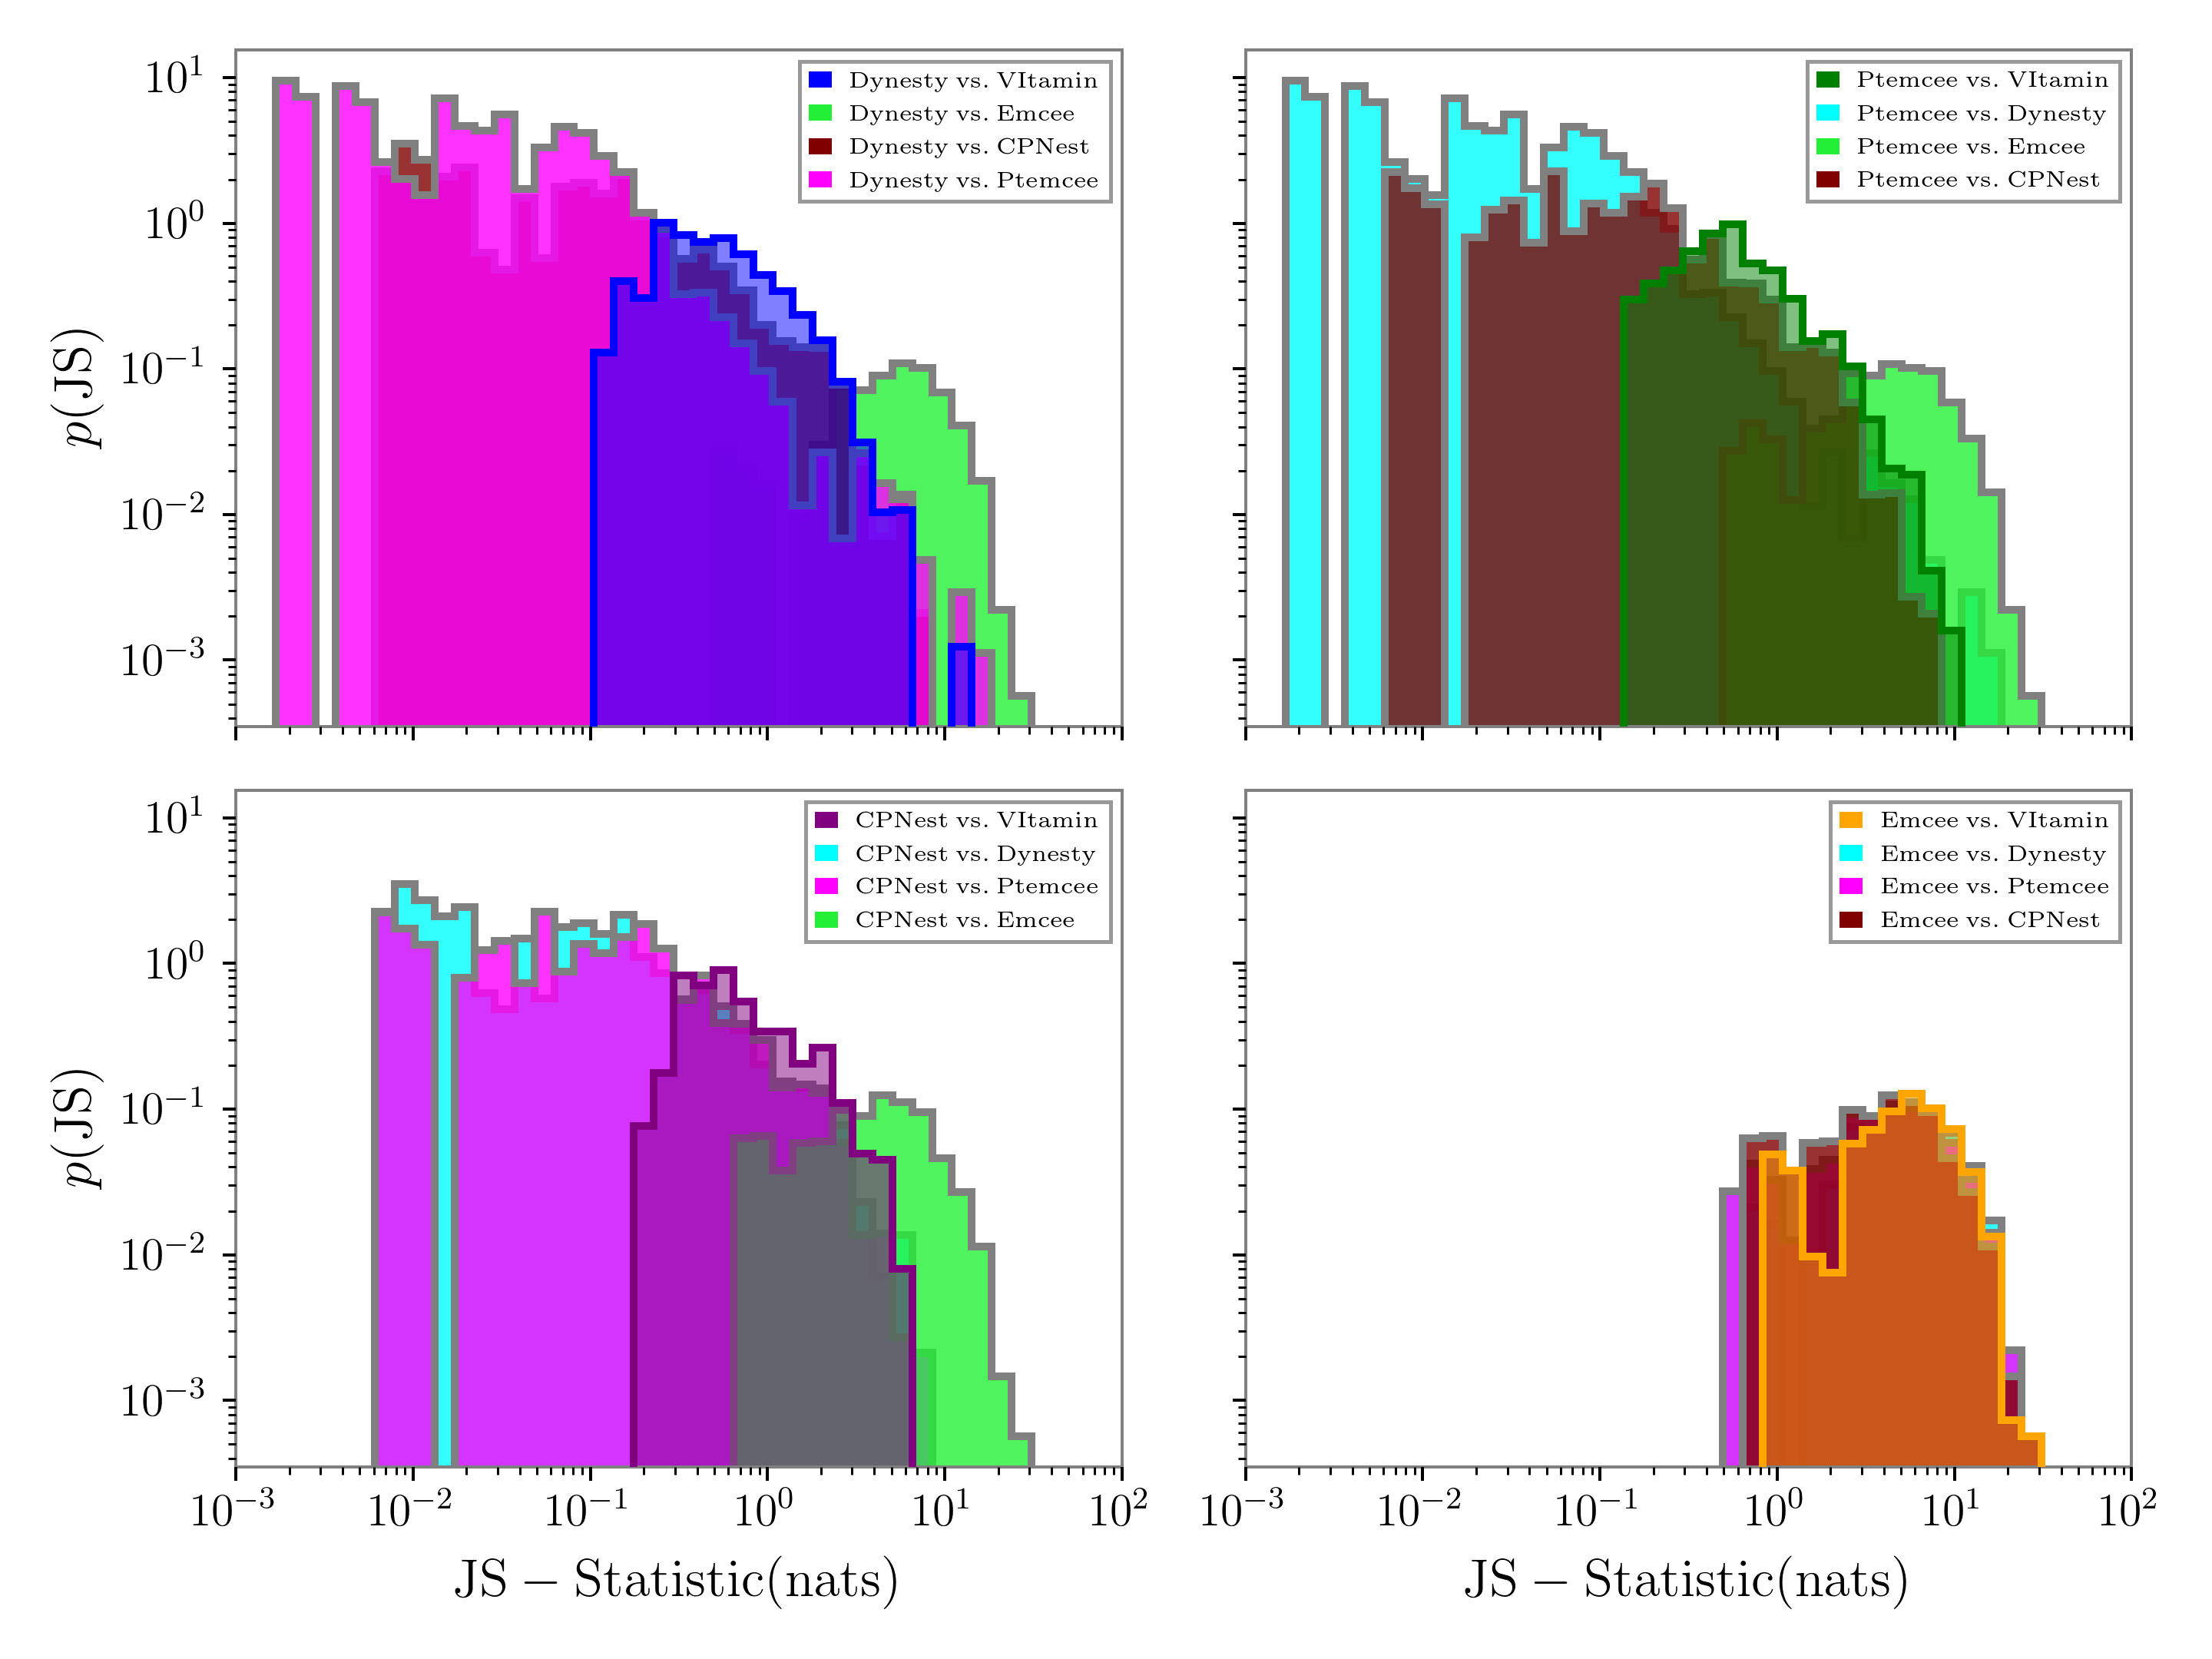
\includegraphics[width=\textwidth]{hist-JS.png}
    \caption[Distributions of the JS-divergence 
    values across 14 parameters between posteriors produced by different
    samplers.]{\label{fig:kl_results} Distributions of \ac{JS}-divergence 
    values between posteriors produced by different samplers. In each 
    panel we show the distribution of \ac{JS}-divergences computed 
    between a single benchmark sampler and every other benchmark sampler 
    over all 250 \ac{GW} test cases (grey histogram outlines). 
    Also plotted in each 
    panel are the corresponding \ac{JS}-divergence distributions 
    between the single benchmark sampler and the \texttt{VItamin} 
    outputs (colored histogram outlines).}

\end{figure*}


\begin{figure}
    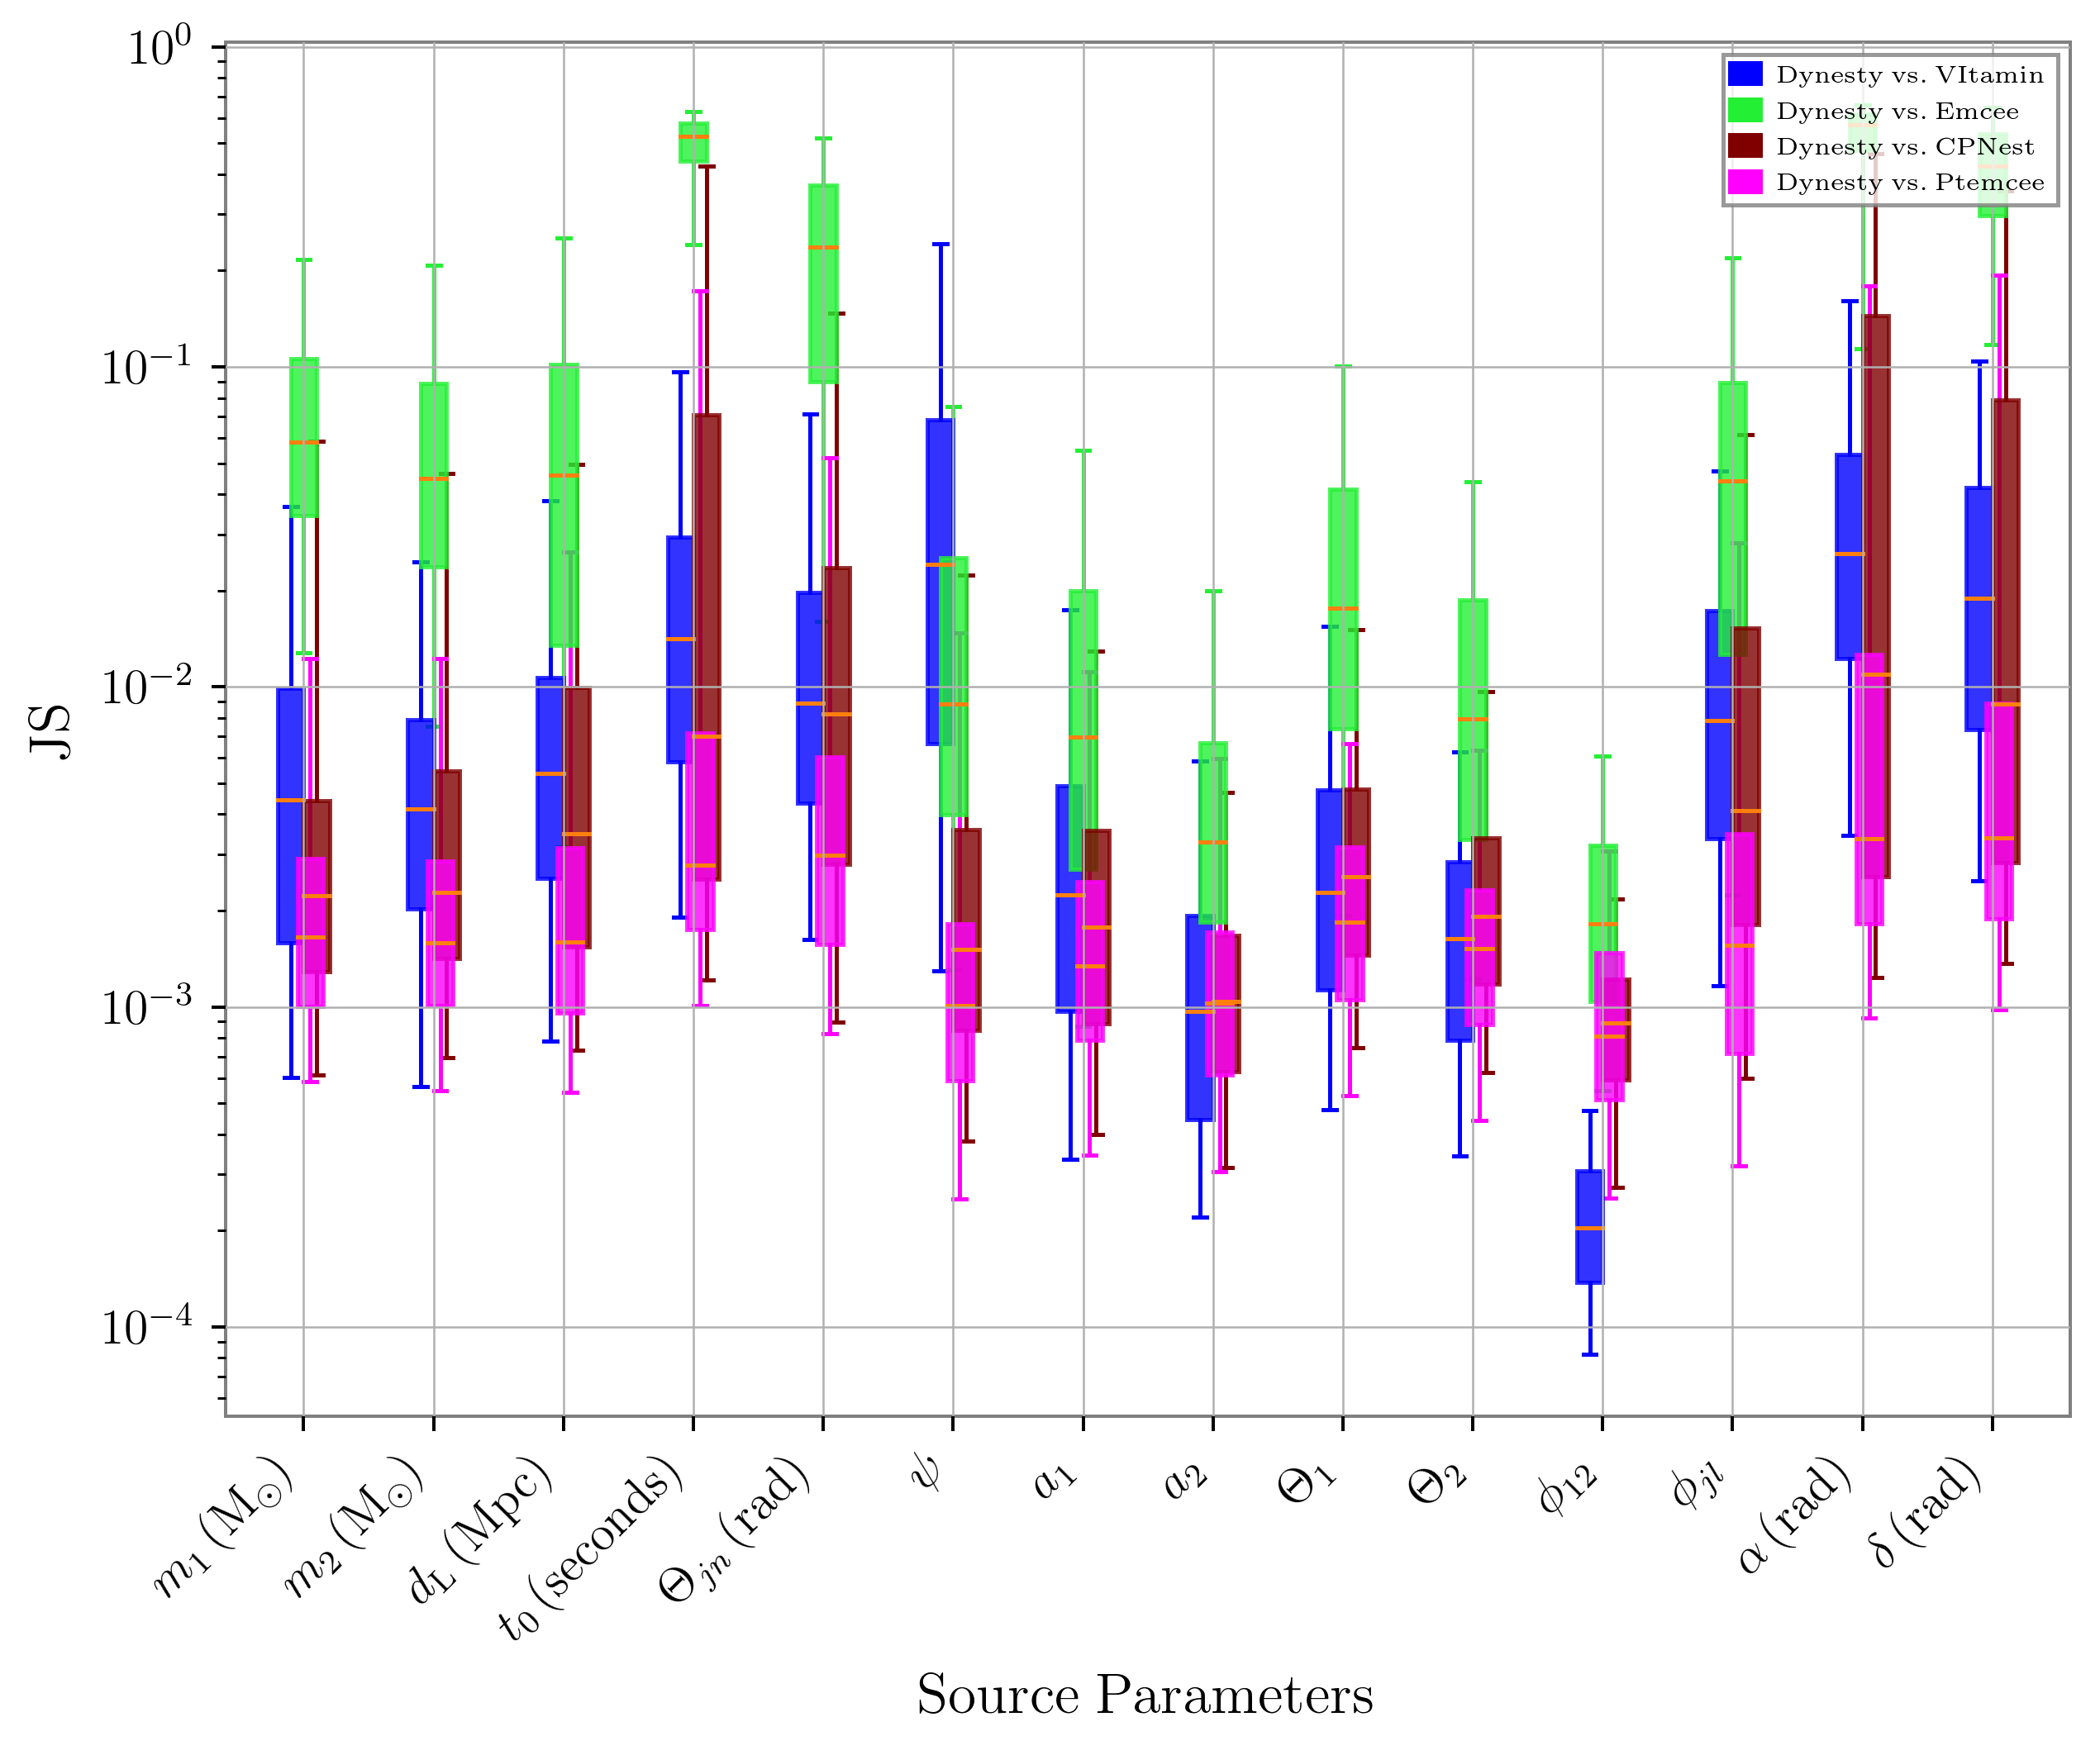
\includegraphics[width=\columnwidth]{figures/JS_IndiPar_dynesty.png}
    \caption[JS divergences of individual source parameters for \texttt{Dynesty} against all other approaches.]{\label{fig:JS_indi_par_dynesty} We show JS divergence values for all 250 test samples as a function of test sample source parameter for \texttt{Dynesty} against every other sampling approach. Each sampler method vs. another sampler method are denoted as different colors. The lower and upper end of boxes represent the 25th and 75th percentile credible regions respectively. The lower and upper end of the whiskers represent the 5th and 95th percentile credible regions. The orange lines are representative of the median JS values for each pair of compared samplers.}
\end{figure}

%
% discuss the speed of the analysis
%
The dominating computational cost of running \texttt{VItamin} lies 
in the training time, which can take $\mathcal{O}(7)$ days~\chris{There is the opportunity to include a simple study of the benchmark evolution as a function of both total loss and wall-clock time. You already have the plots for this.} 
to complete. Completion is determined by comparing posteriors 
produced by the machine learning model and those of 
\texttt{Bilby} iteratively during training~\chris{well, kind of. If we got perfect overlap then yes we would stop at that point. However, as we now know, the loss is still evolving even at 50K epochs. A really nice thing to add would be the true ultimate H value that we can theoretically achieve computed using the dynesty evidence and the sample likelihoods and priors}. We 
additionally assess whether the cost curves (Fig.~\ref{fig:loss_log}) 
have converged, such that 
their slope is near-zero~\chris{true, but see previous comment}.

We stress that once trained, there is no need to retrain the network 
unless the user wishes to use different priors $p(x)$ or assume 
different noise characteristics. The speed at which posterior 
samples are generated for all samplers used, including \texttt{VItamin}, 
is shown in Table~\ref{Tab:speed}. Run-time for the benchmark samplers is 
defined as the time to complete their analyses when configured using 
the parameter choices defined in Table~\ref{Tab:sampler_params}. 
For \texttt{VItamin}, the run-time is defined as the total time to 
produce $8000$ samples. To be clear, this does not include 
the $\mathcal{7}$ days required to train the network. For our test 
case of \ac{BBH} signals \texttt{VItamin} produces samples from the 
posterior at a rate which is $\sim 6$ orders of magnitude faster than 
our benchmark analysis using current inference techniques, 
representing a dramatic speed-up in performance.

%\chris{One more thing to add, especially if the other KL, AD, and PP plots
%aren't convincing, is a plot displaying 1D confidence bounds compared between
%bilby and VItamin. Imagine a plot with the x-axis as distance and the y-axis
%steps through test data with increasing true distance. for each test data you
%plot 2 error bars horizontally (one for bilby and one for VItamin) spanning the
%range of 90\% confidence. You would hopefully get nearly identical pairs of
%errorbars stacked vertically. Technically you could do this for all parameters
%(and you should) but we might only put one of the plots in the paper (if at
%all).}

%
% I feel the need, the need for speed, table
% 
\begin{table}
%\centering
\caption[Durations required to produced samples from 
 different posterior approaches.]{Durations required to produce 
 samples from each of the different posterior sampling approaches.}
\begin{minipage}{\linewidth}
\begin{center}
\begin{tabular}[t]{lcccc} 
\toprule
\multirow{2}{*}{sampler} & \multicolumn{3}{c}{run time (s)} & \multirow{2}{*}{ratio
$\displaystyle\frac{\tau_{\text{VItamin}}}{\tau_{X}}$} \\
& min & max & median & \\
\hline
\texttt{Dynesty}\footnote{The benchmark samplers all produced
$\mathcal{O}(8000)$ samples dependent on the default sampling parameters
used.}~\cite{dynesty} & 21564 & 261268 & 45607
\footnote{We note that there are a growing number of specialised
techniques~\cite{2016PhRvD..94d4031S,2019PhRvD..99h4026W,2019PhRvD.100d3030T,PhysRevD.92.023002} designed to speed up traditional sampling algorithms that could be used to reduce the runtimes quoted here by $\mathcal{O}(1-2)$ orders of magnitude.}
%\footnote{The reader may note that benchmark sampler run times are a few orders
%of magnitude lower than what is typical of a complete \ac{BBH} analysis
%($\mathcal{O}(10^{4} -10^{5})$ seconds). This is primarily due our use of a
%reduced parameter space, low sampling rate and choice of sampler
%hyperparameters.} 
& $2.2\times 10^{-6}$ \\
\texttt{emcee}~\cite{emcee} & 16712 & 39930 & 19821 & $5.1\times 10^{-6}$ \\
\texttt{ptemcee}~\cite{ptemcee} & 2392 & 501632 & 41151.0 & $2.4\times 10^{-6}$ \\
\texttt{CPNest}~\cite{cpnest} & 10309 & 437008 & 83807 & $1.2\times 10^{-6}$ \\
\texttt{VItamin}\footnote{For the \texttt{VItamin} sampler $8000$ samples are
produced as representative of a typical posterior. The run time is independent
of the signal content in the data and is therefore constant for all test cases.} & \multicolumn{3}{c}{\bm{$1\times10^{-1}$}} & 1 \\
\botrule
\end{tabular}
\end{center}
\label{Tab:speed}
\end{minipage}
\end{table}

%
% word count ~960 - approx 9.6 words per line
%

%%%%%%%%%%%%%%%%%%%%%%%%%%%%%%%%%%%%%%%%%%%%%%%%%%%%%%%%%%%%%%%%%%%%%%
%%%%%%%%%%%%%%%%%%%%%%%%%%%%%%%%%%%%%%%%%%%%%%%%%%%%%%%%%%%%%%%%%%%%%%





%%%%%%%%%%%%%%%%%%%%%%%%%%%%%%%%%%%%%%%%%%%%%%%%%%%%%%%%%%%%%%%%%%%%%%%%%%%%%%
%%%%%%%%%%%%%%%%%%%%%%%%%%%%%%%%%%%%%%%%%%%%%%%%%%%%%%%%%%%%%%%%%%%%%%%%%%%%%%
%%%%%%%%%%%%%%%%%%%%%%%%%%%%%%%%%%%%%%%%%%%%%%%%%%%%%%%%%%%%%%%%%%%%%%%%%%%%%%

%\subsection{Additional Jensen--Shannon Divergence Plots Computed on Individual Source Parameters}

%
% Individual source parameter JS divergences
%

%We provide additional \ac{JS}-divergence figures of merit in 
%Figs.~\ref{fig:JS_indi_par_cpnest}, \ref{fig:JS_indi_par_emcee},
%and~\ref{fig:JS_indi_par_ptemcee} where we plot the \ac{JS}-divergence 
%values for each \ac{GW} source parameter across all 
%Bayesian sampler approaches.
%
% Discuss CPNest plot
%

%In Fig. \ref{fig:JS_indi_par_cpnest}, \texttt{CPNest} is highlighted against 
%all other sampler approaches (including \texttt{VItamin}). It can be seen 
%that both \texttt{CPnest} vs. \texttt{Dynesty} and \texttt{CPnest} vs. 
%\texttt{Ptemcee} are in strong agreement with each other (although with broad 
%credibility regions on $t_0$, $\theta_{jn}$, $\alpha$, $\delta$). \texttt{CPNest} 
%vs. \texttt{VItamin} is also in strong agreement with \texttt{CPnest} vs. \texttt{Dynesty} and \texttt{CPnest} vs. \texttt{Ptemcee}, but it does show some 
%disagreement on $m_1$, $m_2$ and $\psi$. \texttt{CPNest} vs. \texttt{Emcee} is 
%generally in disagreement with all other approaches.

\begin{figure}
    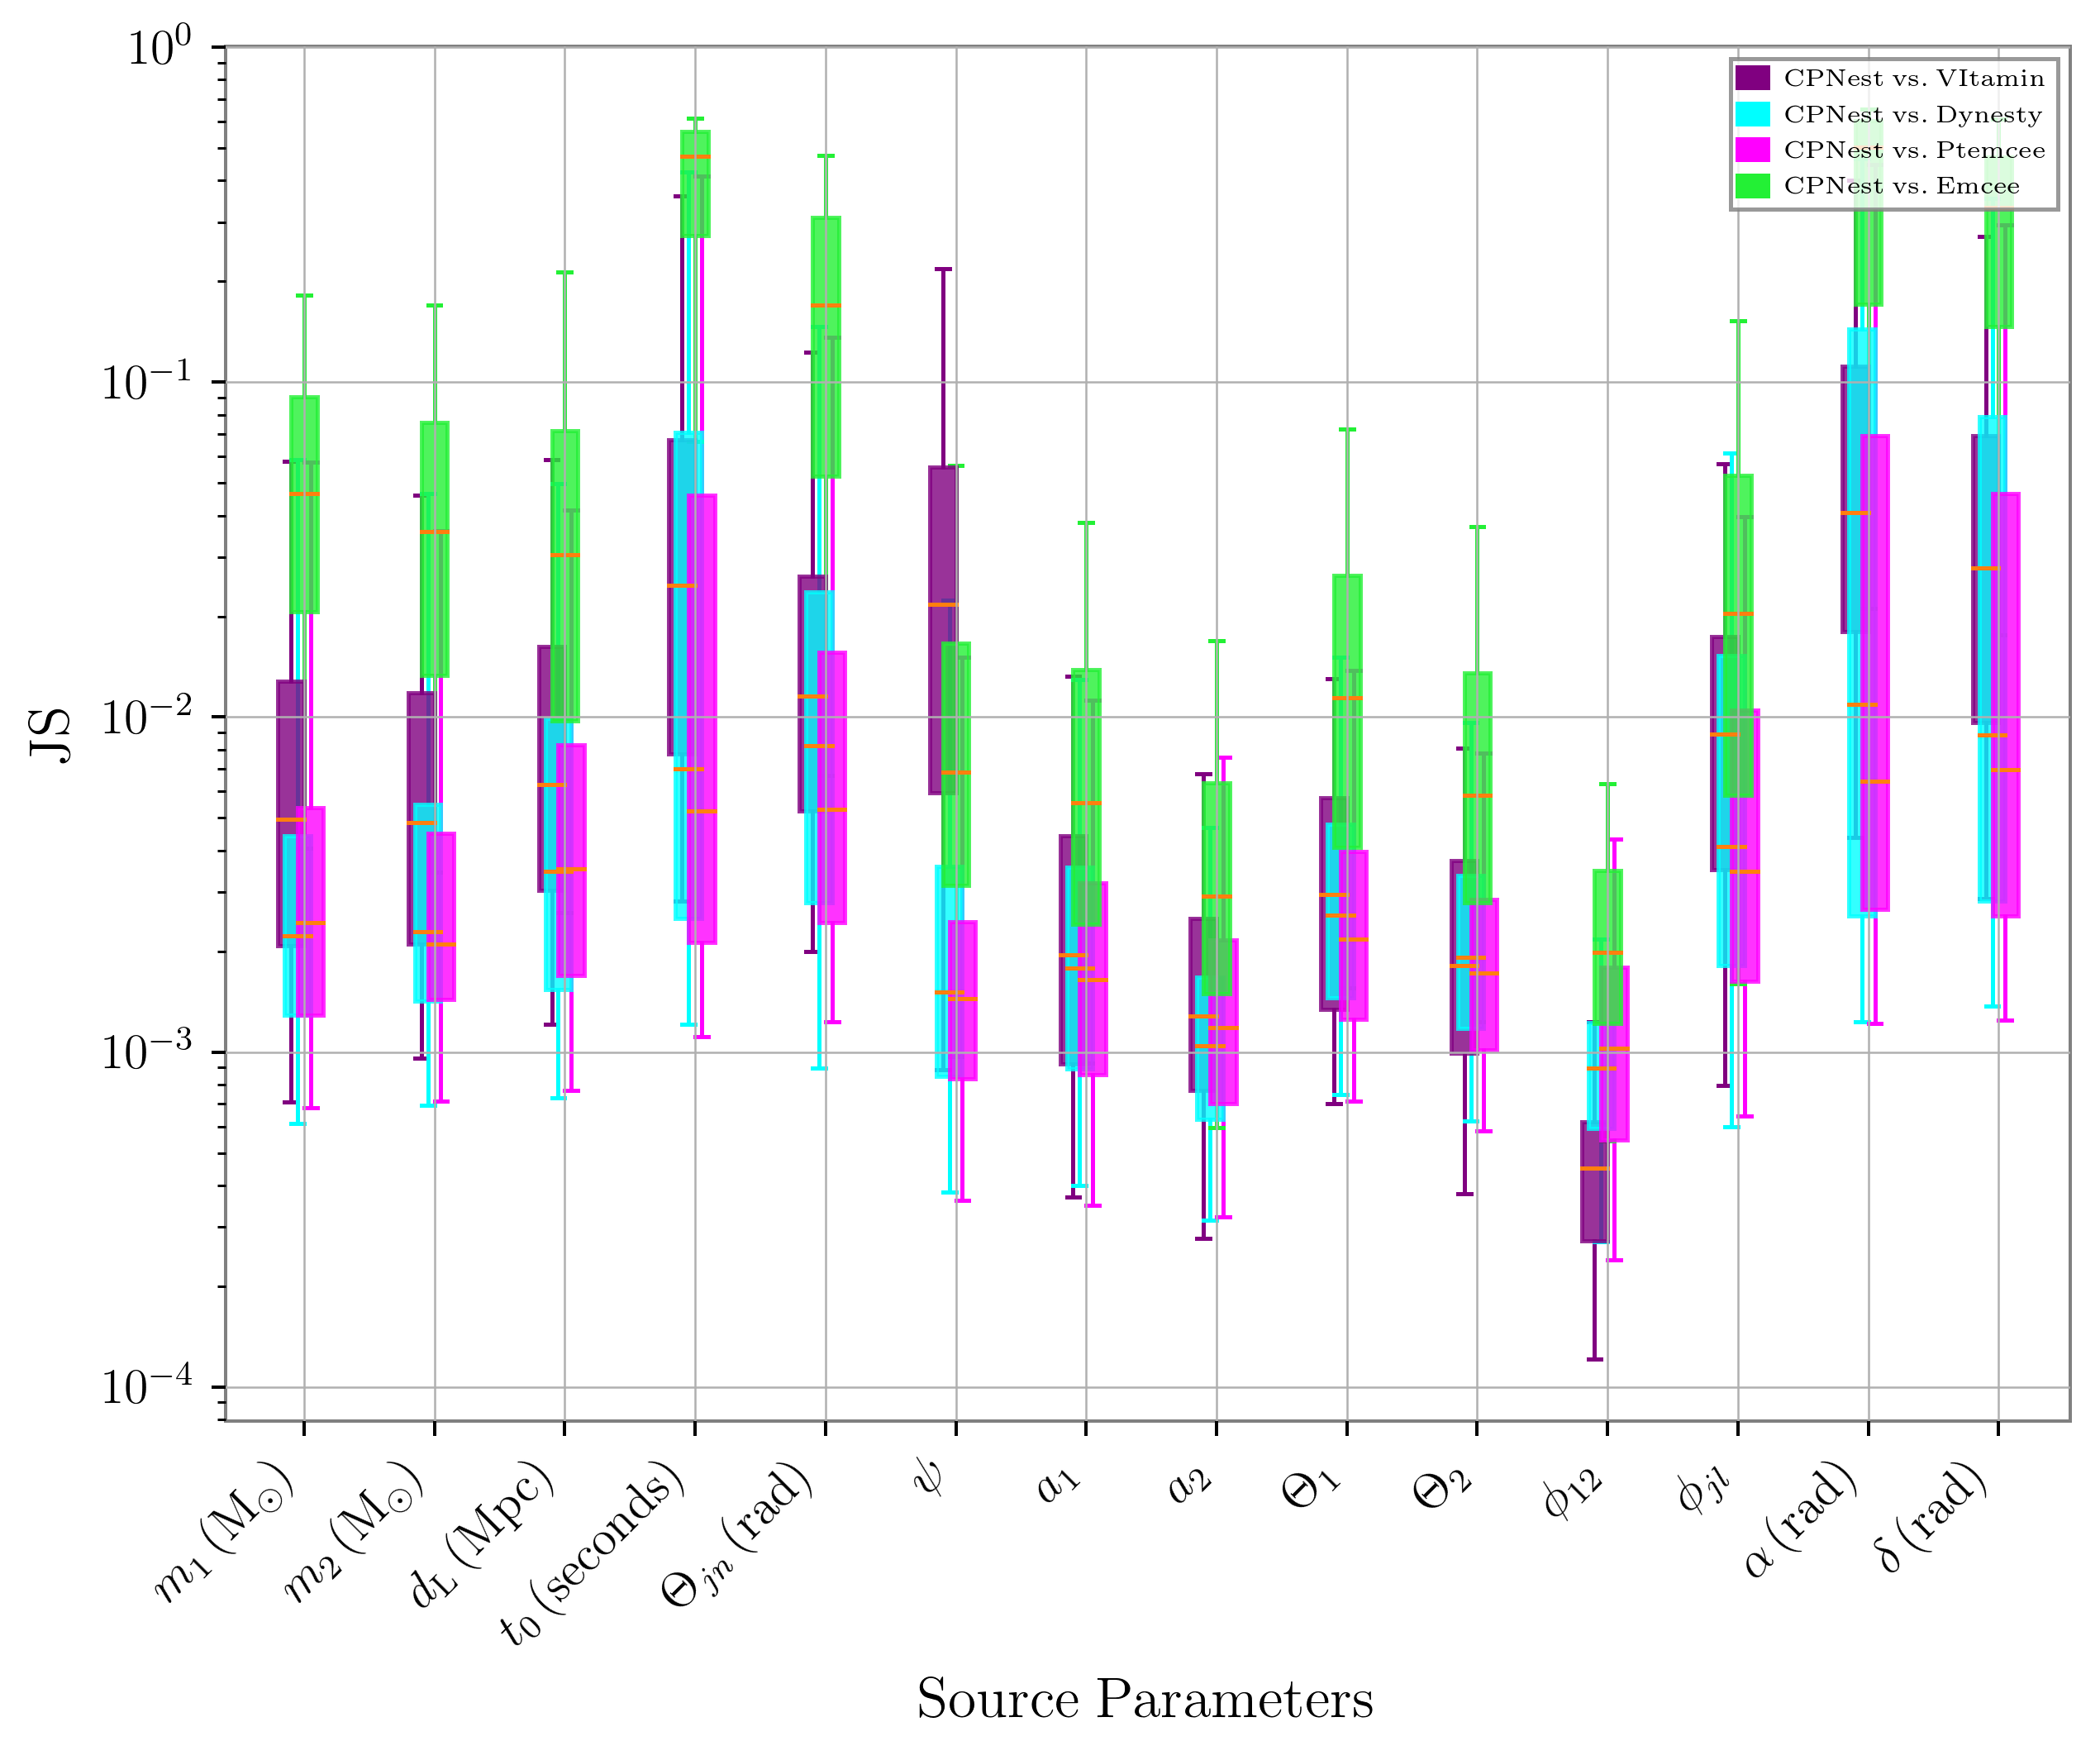
\includegraphics[width=\columnwidth]{figures/JS_IndiPar_cpnest.png}
    \caption[JS divergences of individual source parameters for \texttt{CPNest} against all other approaches.]{\label{fig:JS_indi_par_cpnest} We show JS divergence values for all 250 test samples as a function of test sample source parameter for \texttt{CPnest} against every other sampling approach. Each sampler method vs. another sampler method are denoted as different colors. The lower and upper end of boxes represent the 25th and 75th percentile credible regions respectively. The lower and upper end of the whiskers represent the 5th and 95th percentile credible regions. The orange lines are representative of the median JS values for each pair of compared samplers.}
\end{figure}

%
% Discuss Emcee JS indi par plot
%

%Fig. \ref{fig:JS_indi_par_emcee} highlights the \texttt{Emcee} sampler 
%vs. all other approaches including \texttt{VItamin}. In Fig. 
%\ref{fig:JS_indi_par_emcee} it can be seen that \texttt{Emcee} has equal 
%overlap against all other sampler approaches. Given the high JS values 
%of \texttt{Emcee} vs. all other approaches, this indicates that \texttt{Emcee} 
%has found difficulty converging on many of the test sample cases. This is 
%expected given that it is well known that \texttt{Emcee} generally difficult 
%to tune for proper convergence.

\begin{figure}
    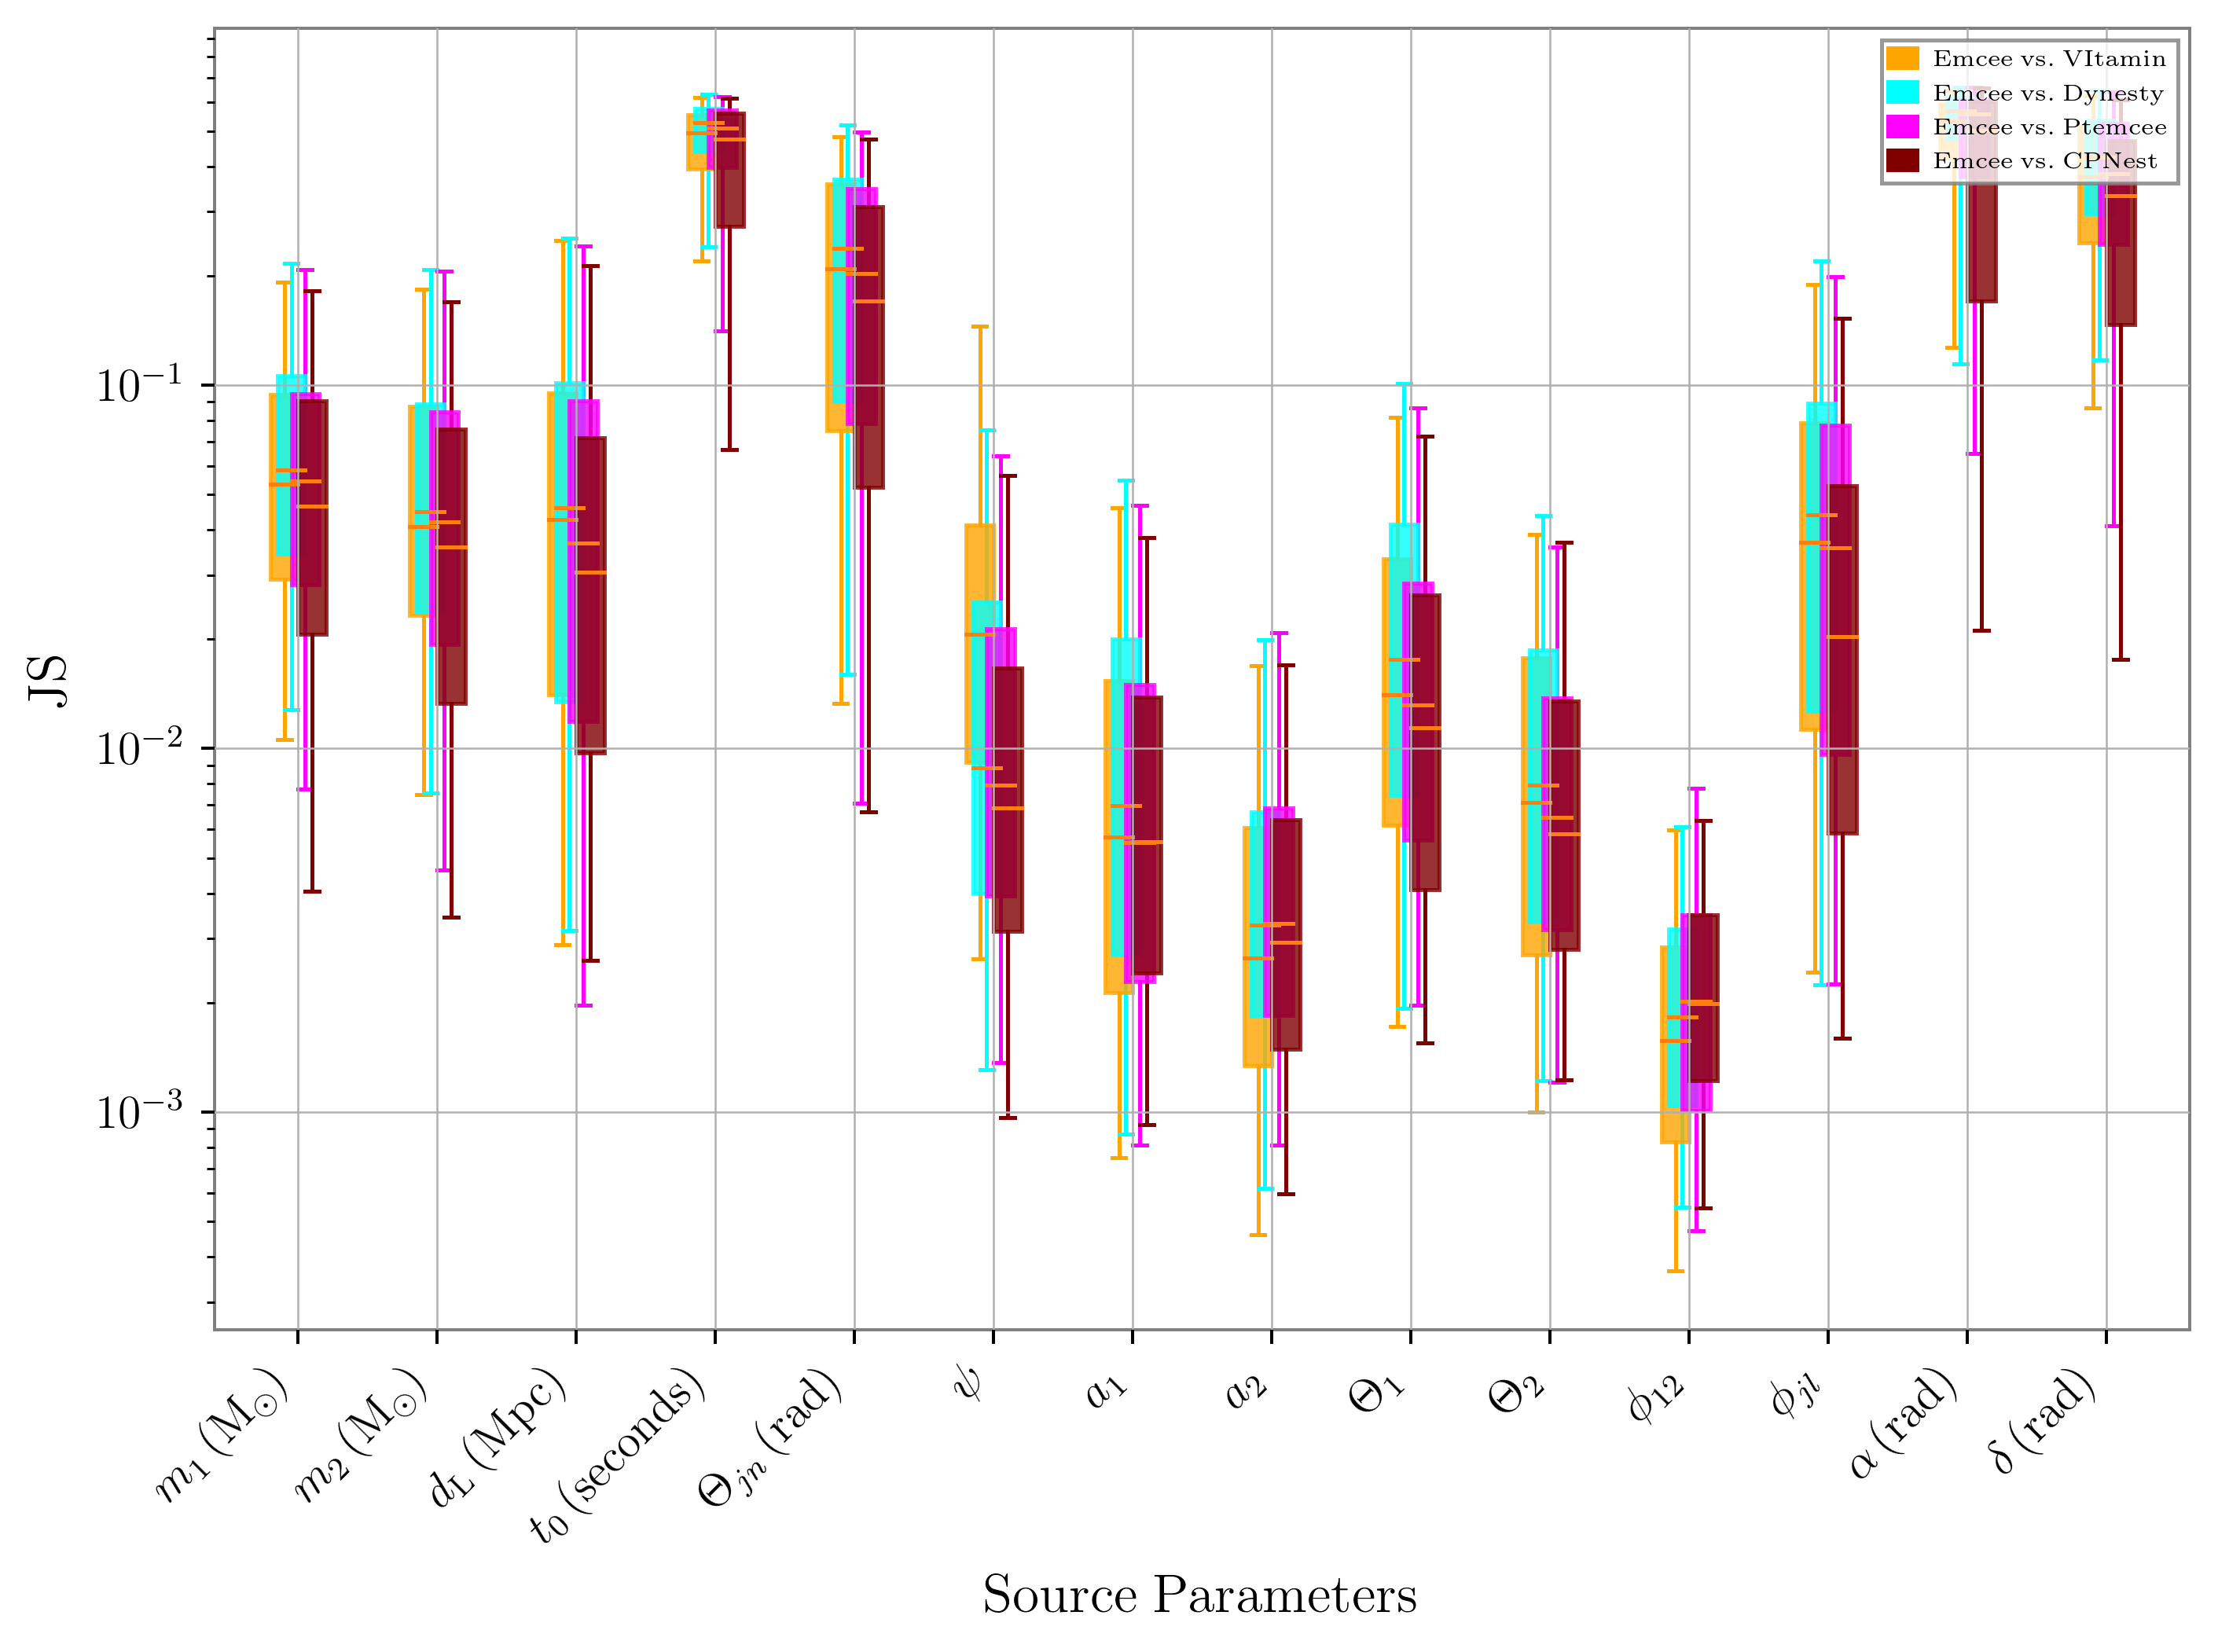
\includegraphics[width=\columnwidth]{figures/JS_IndiPar_emcee.png}
    \caption[JS divergences of individual source parameters for \texttt{Emcee} against all other approaches.]{\label{fig:JS_indi_par_emcee} We show JS divergence values for all 250 test samples as a function of test sample source parameter for \texttt{emcee} against every other sampling approach. Each sampler method vs. another sampler method are denoted as different colors. The lower and upper end of boxes represent the 25th and 75th percentile credible regions respectively. The lower and upper end of the whiskers represent the 5th and 95th percentile credible regions. The orange lines are representative of the median JS values for each pair of compared samplers. We see here that \texttt{VItamin} performs to within a degree of accuracy which is consistent with other Bayesian samplers when looking at predictions on an individual source parameter basis.}
\end{figure}

%
% Discuss Ptemcee JS indi par plot
%

%Fig. \ref{fig:JS_indi_par_ptemcee} highlights \texttt{Ptemcee} vs. all 
%other sampler approaches. In Fig. \ref{fig:JS_indi_par_ptemcee} we see 
%that \texttt{Ptemcee} vs. \texttt{Dynesty} and \texttt{Ptemcee} vs. 
%\texttt{CPNest} closely match each other with the exception of slight 
%disagreement on $t_0$, $\theta_{jn}$ and $\phi_{jl}$ (with broader credibility %regions on \texttt{Ptemcee} 
%vs. \texttt{CPNest}). \texttt{Ptemcee} vs. \texttt{VItamin} in dark green 
%also closely matches the \texttt{Ptemcee} vs. \texttt{Dynesty} and %\texttt{Ptemcee} vs. \texttt{CPNest} results with slightl higher JS values 
%accross all source parameter values other than the spin parameters. 
%\texttt{Emcee} is in strong misalignment with all other approaches.

\begin{figure}
    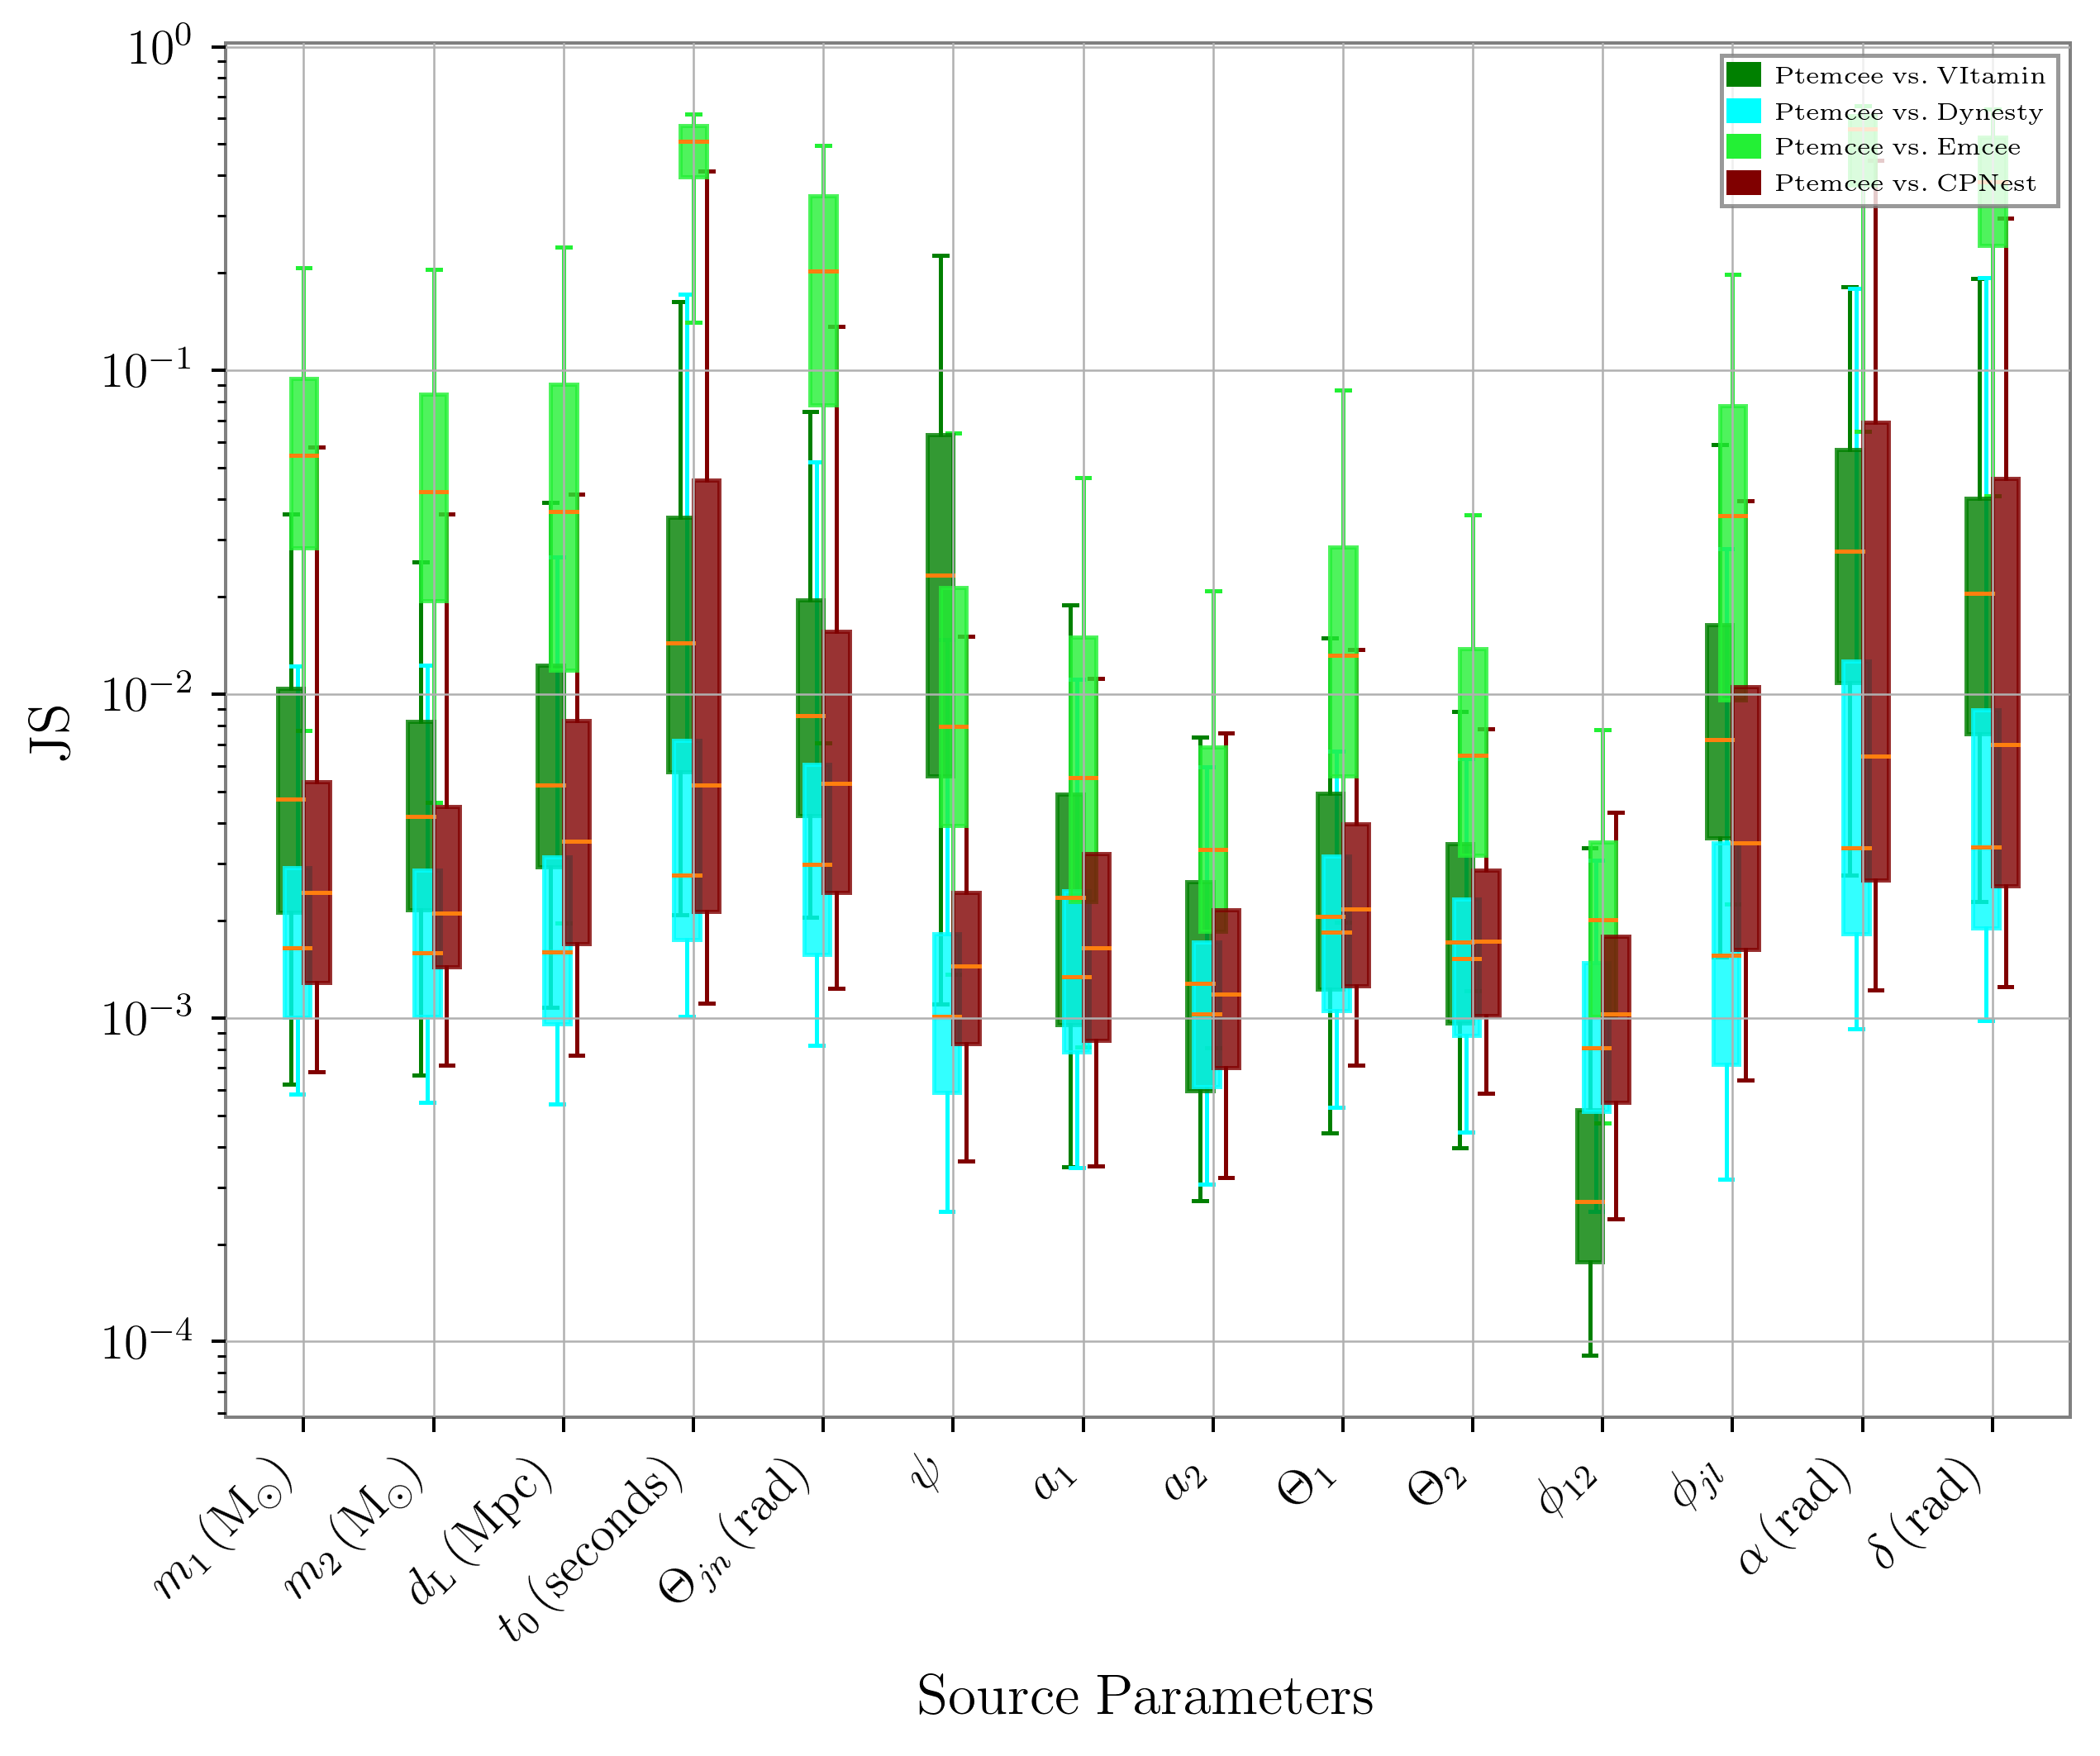
\includegraphics[width=\columnwidth]{figures/JS_IndiPar_ptemcee.png}
    \caption[JS divergences of individual source parameters for \texttt{Ptemcee} against all other approaches.]{\label{fig:JS_indi_par_ptemcee} We show JS divergence values for all 250 test samples as a function of test sample source parameter for \texttt{Ptemcee} against every other sampling approach. Each sampler method vs. another sampler method are denoted as different colors. The lower and upper end of boxes represent the 25th and 75th percentile credible regions respectively. The lower and upper end of the whiskers represent the 5th and 95th percentile credible regions. The orange lines are representative of the median JS values for each pair of compared samplers. We see here that \texttt{VItamin} performs to within a degree of accuracy which is consistent with other Bayesian samplers when looking at predictions on an individual source parameter basis.}
\end{figure}

%It is evident in Fig's \ref{fig:JS_indi_par_cpnest}, %\ref{fig:JS_indi_par_emcee}, \ref{fig:JS_indi_par_ptemcee} that JS values for %individual source 
%parameters of \texttt{VItamin} against all other sampler is generally 
%consistent with all other samplers against themselves. This is an important 
%point because it indicates that our \ac{ML} approach is able 
%to produce Bayesian posteriors to within an accuracy which is at a similar 
%level of other Bayesian samplers, using the same individual source 
%parameter figure of merit used for other comparison studies in the Bayesian 
%\ac{GW} parameter estimation literature %\cite{1811.02042,2008.03312,PhysRevD.102.104057}. What is also 
%interesting to note is the level of disagreement of other Bayesian samplers 
%with themselves. This disagreement is especially prominent with regards 
%to source parameters $t_0$, $\theta_{jn}$, $\phi_{jl}$, $\alpha$, and $\delta$.
%Although \texttt{Emcee} results are fairly poor in comparison with other 
%approaches, they are a useful benchmark for indicating underperformance. 


\section{Additional Supplemental \texttt{VItamin} Results and Analysis}

In the following sections we will discuss additional analysis which supplement the 
main 
results of this chapter including: 
training 
set \ac{SNR} distribution and it's  relationship to the 
performance of \texttt{VItamin}, as well as the structure and behavior 
of the \ac{CVAE} latent space and it's relationship with 
the predicted posterior distributions. 

\subsection{Jensen-Shannon Divergence as a Function of Signal-to-Noise Ratio}

Over the course of the work carried out in this chapter there was 
some verbal discussion~\chris{I think you should rephrase how you 
want to introduce this section} on the possibility that high \ac{SNR} 
signals could be a limiting factor with regards to the performance of the 
neural network model. It was originally hypothesized that 
due to the low number of high \ac{SNR} signals in our training set 
(as seen in Fig.~\ref{fig:VItamin_TrainingSet_SNR_Dist}), that the 
network would perform worse on high \ac{SNR} signals. This 
hypothesis is supported by the well known understanding in \ac{ML} 
literature that less available data in specific regions of the 
parameter space can cause a neural network model to underfit to those 
regions \cite{Goodfellow-et-al-2016}. In Fig.~\ref{fig:JS_vs_SNR_dynesty}
the \ac{JS}-divergence for individual test sample cases 
of \texttt{VItamin} vs. \texttt{Dynesty} as a function of \ac{SNR}. 
Each plus sign is representative of individual test cases and 
different colors correspond to each interferometer. 

\begin{figure}
    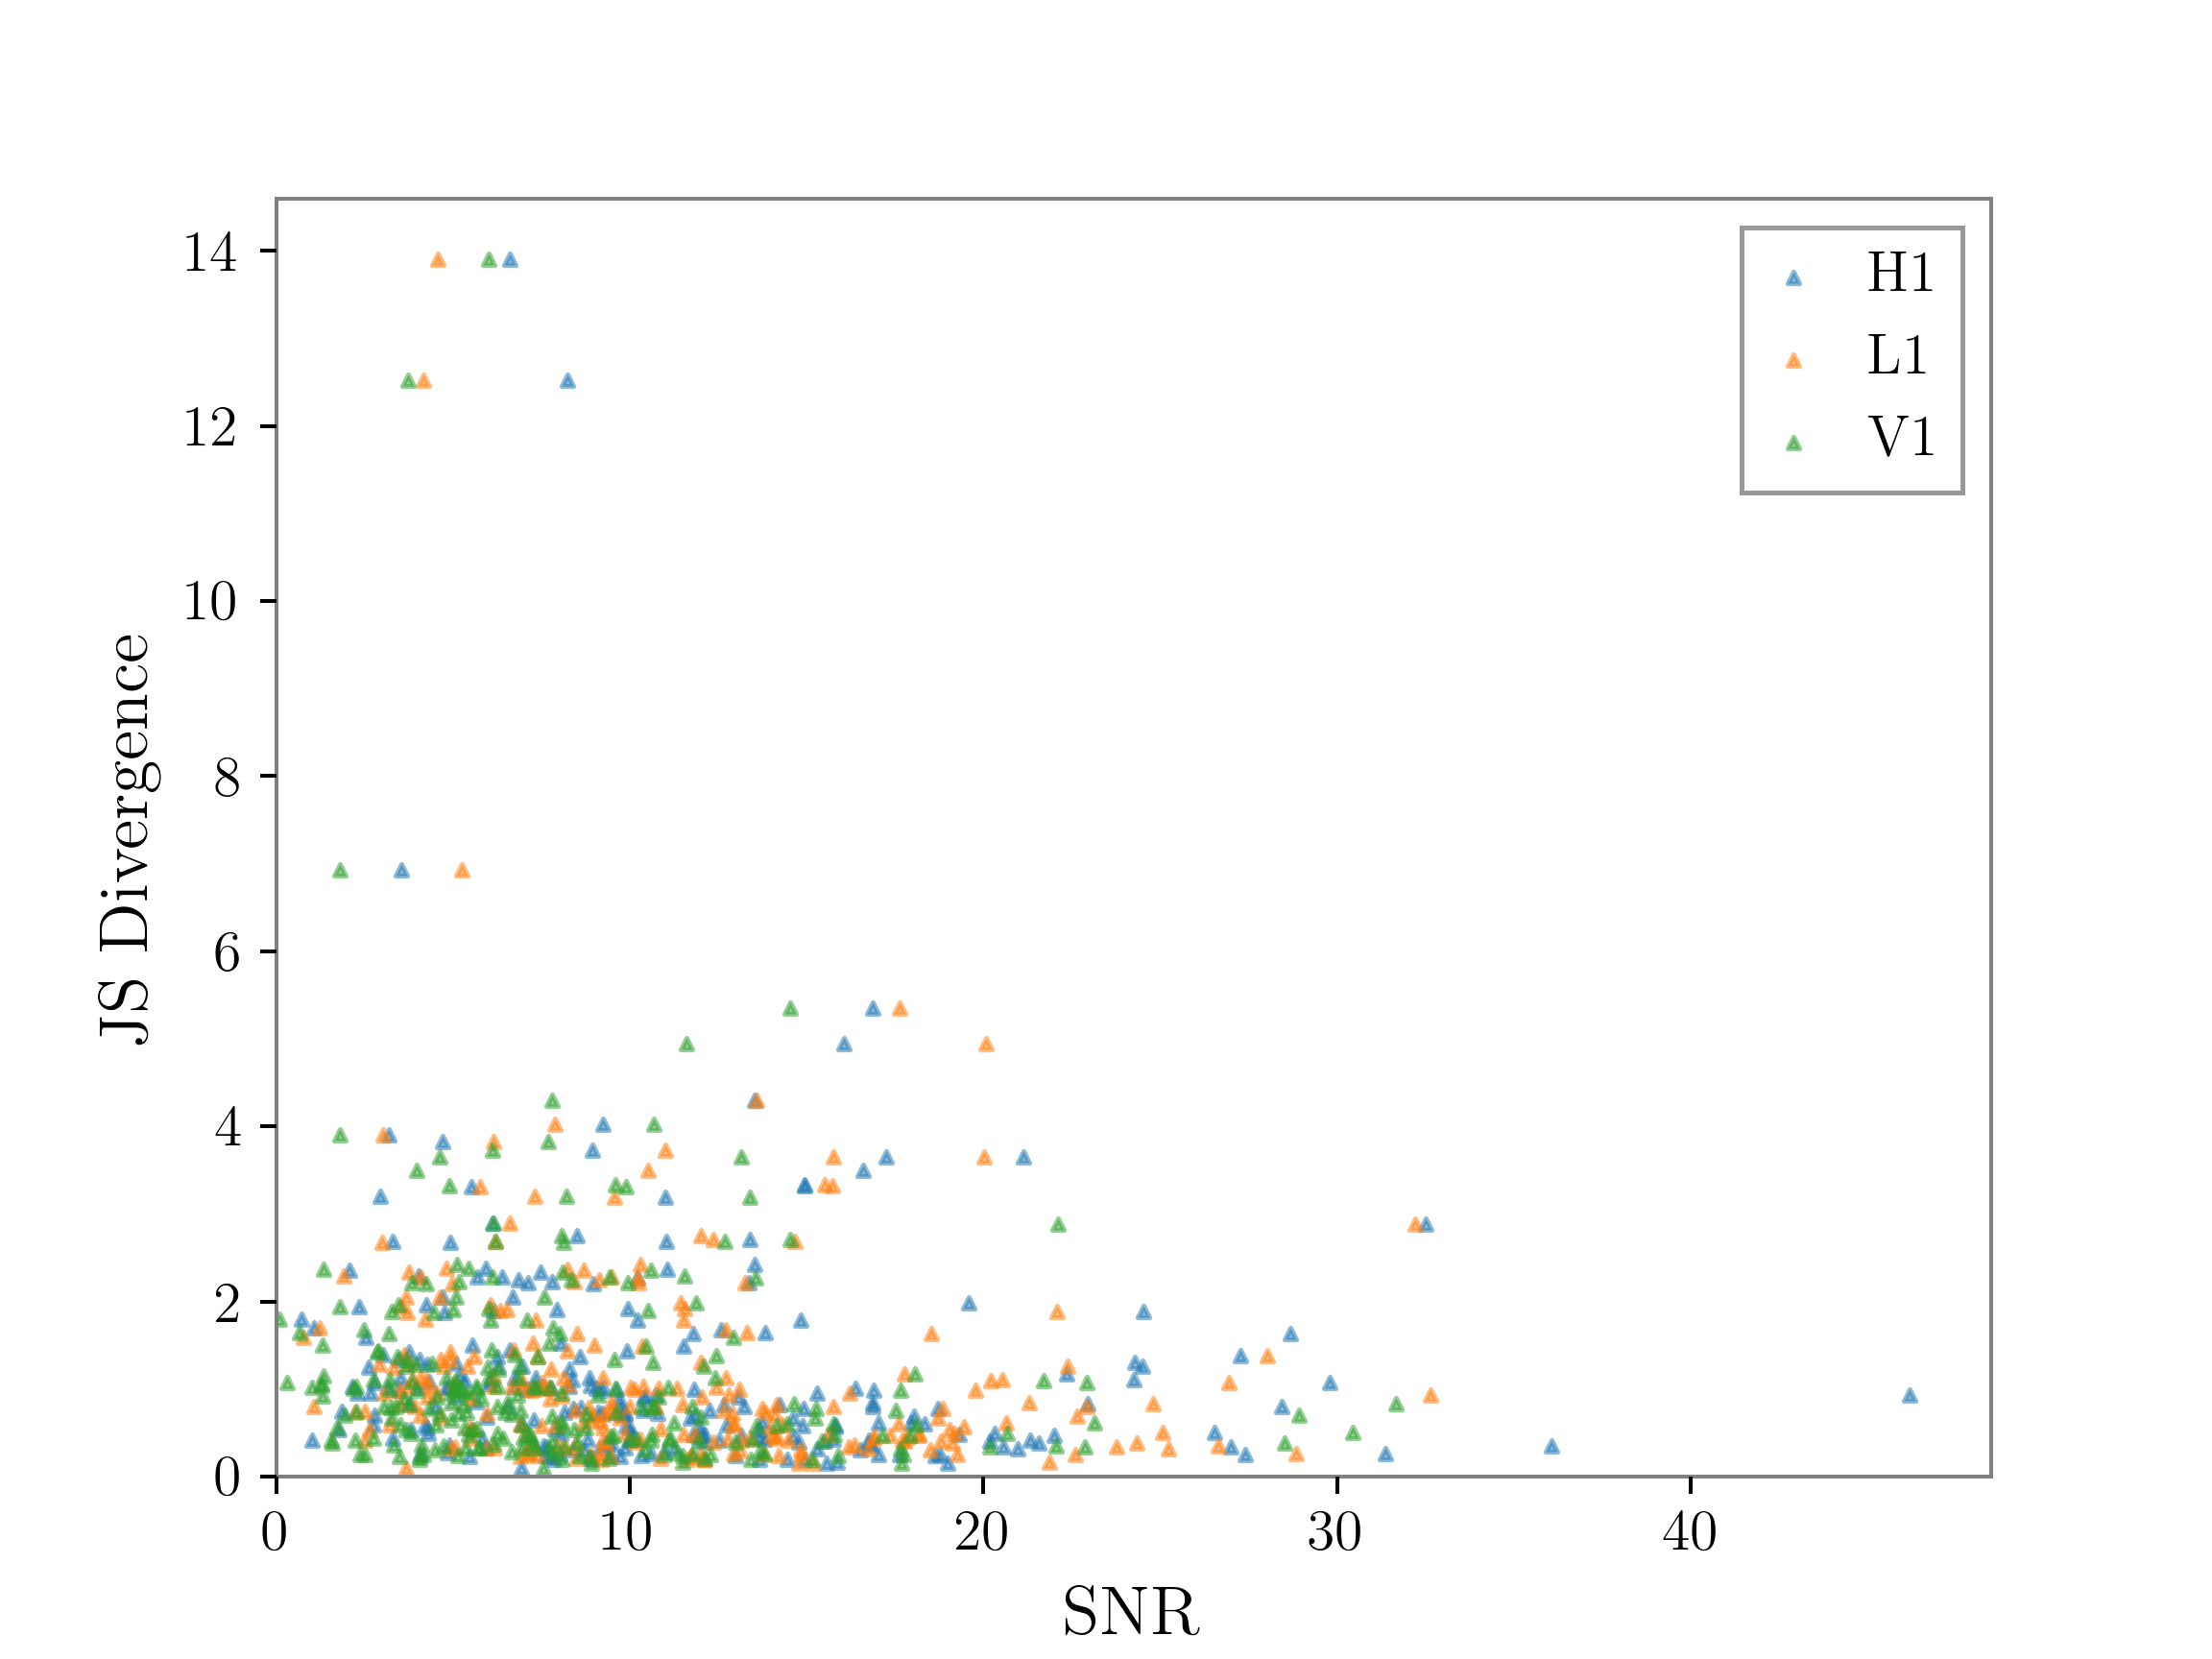
\includegraphics[width=\columnwidth]{figures/JS_vs_SNR.png}
    \caption[14-dimensional JS-divergences of \texttt{Dynesty} vs. \texttt{VItamin} as a function of individual detector optimal SNR.]{\label{fig:JS_vs_SNR_dynesty} We show here 14-dimensional 
    \ac{JS}-divergence values of \texttt{Dynesty} vs. \texttt{VItamin} as a function of optimal
    \ac{SNR} (Ch.~\ref{ch:chap_1}, Sec.~\ref{sec:matched_filtering}). Different colours are representative of each of the 3 detectors (H1, L1, V1) used in the analysis. Each triangle symbol represents a different test \ac{GW} case. As can 
    be seen, there does not appear to be a strong positive correlation with \ac{SNR}.}
\end{figure}

We see in Fig. \ref{fig:JS_vs_SNR_dynesty} that there is little to no 
positive correlation between \ac{SNR} and the 14-dimensional \ac{JS}-
divergence; instead, it appears that there is a slight negative 
correlation.

This plot shows that there would be marginal benefit gained from augmenting 
the training set to more strongly emphasise high \ac{SNR} 
signals, and that the neural network may in fact struggle the most 
with low \ac{SNR} events. Given that the highest \ac{JS}-divergence values 
appears to be loosely correlated with low \ac{SNR} values, one might assume 
that this could partially be solved by oversampling our training set 
in the low \ac{SNR} regime. This is not necessarily practical given that 
the prior would then need to be changed and thus the output posterior 
would then need to be resampled to compensate. \hunter{Not sure what to say 
after this.} Even if there were a positive correlation it is unlikely that simply including more high \ac{SNR} signals would be beneficial to the statistical results of the network model as a whole because there are fewer test signals at high \ac{SNR} anyways due to the priors used.~\chris{OK, I think that you need to make these arguments clearer - high SNR was a worry (but why?) - we tested it and it's actually low SNR that does worse - can we fix it by oversampling at low SNR? - well not easily because the prior is the prior - if we change that then we would have to resample the output to compensate - which we actually already do with distance.}

%
% How does vitamin perform with respect to SNR spread? 
%
One other interesting relationship to analyse is that between the 14-dimensional 
\ac{JS}-divergence and the optimal \ac{SNR} spread across all 3 detectors for a 
given \ac{GW} test signal. The \ac{SNR} spread is calculated by taking the difference 
between the maximum and minimum optimal \ac{SNR} values for each test sample. We plot 
the \ac{JS}-divergence as a function of \ac{SNR} spread in Fig.~\ref{fig:14D_JS_SNR-spread} in order 
to gauge whether our neural network model performs worse when 1 or more detectors 
sees the test signal at a lower \ac{SNR} than the other detectors. We see 
in Fig.~\ref{fig:14D_JS_SNR-spread} that there appears to be no positive correlation 
and possibly a very weak negative correlation between the two quantities. This could 
indicate that our model has some difficulties with signals which have an equal amount 
of optimal \ac{SNR} across all detectors.

\begin{figure}
    \centering
    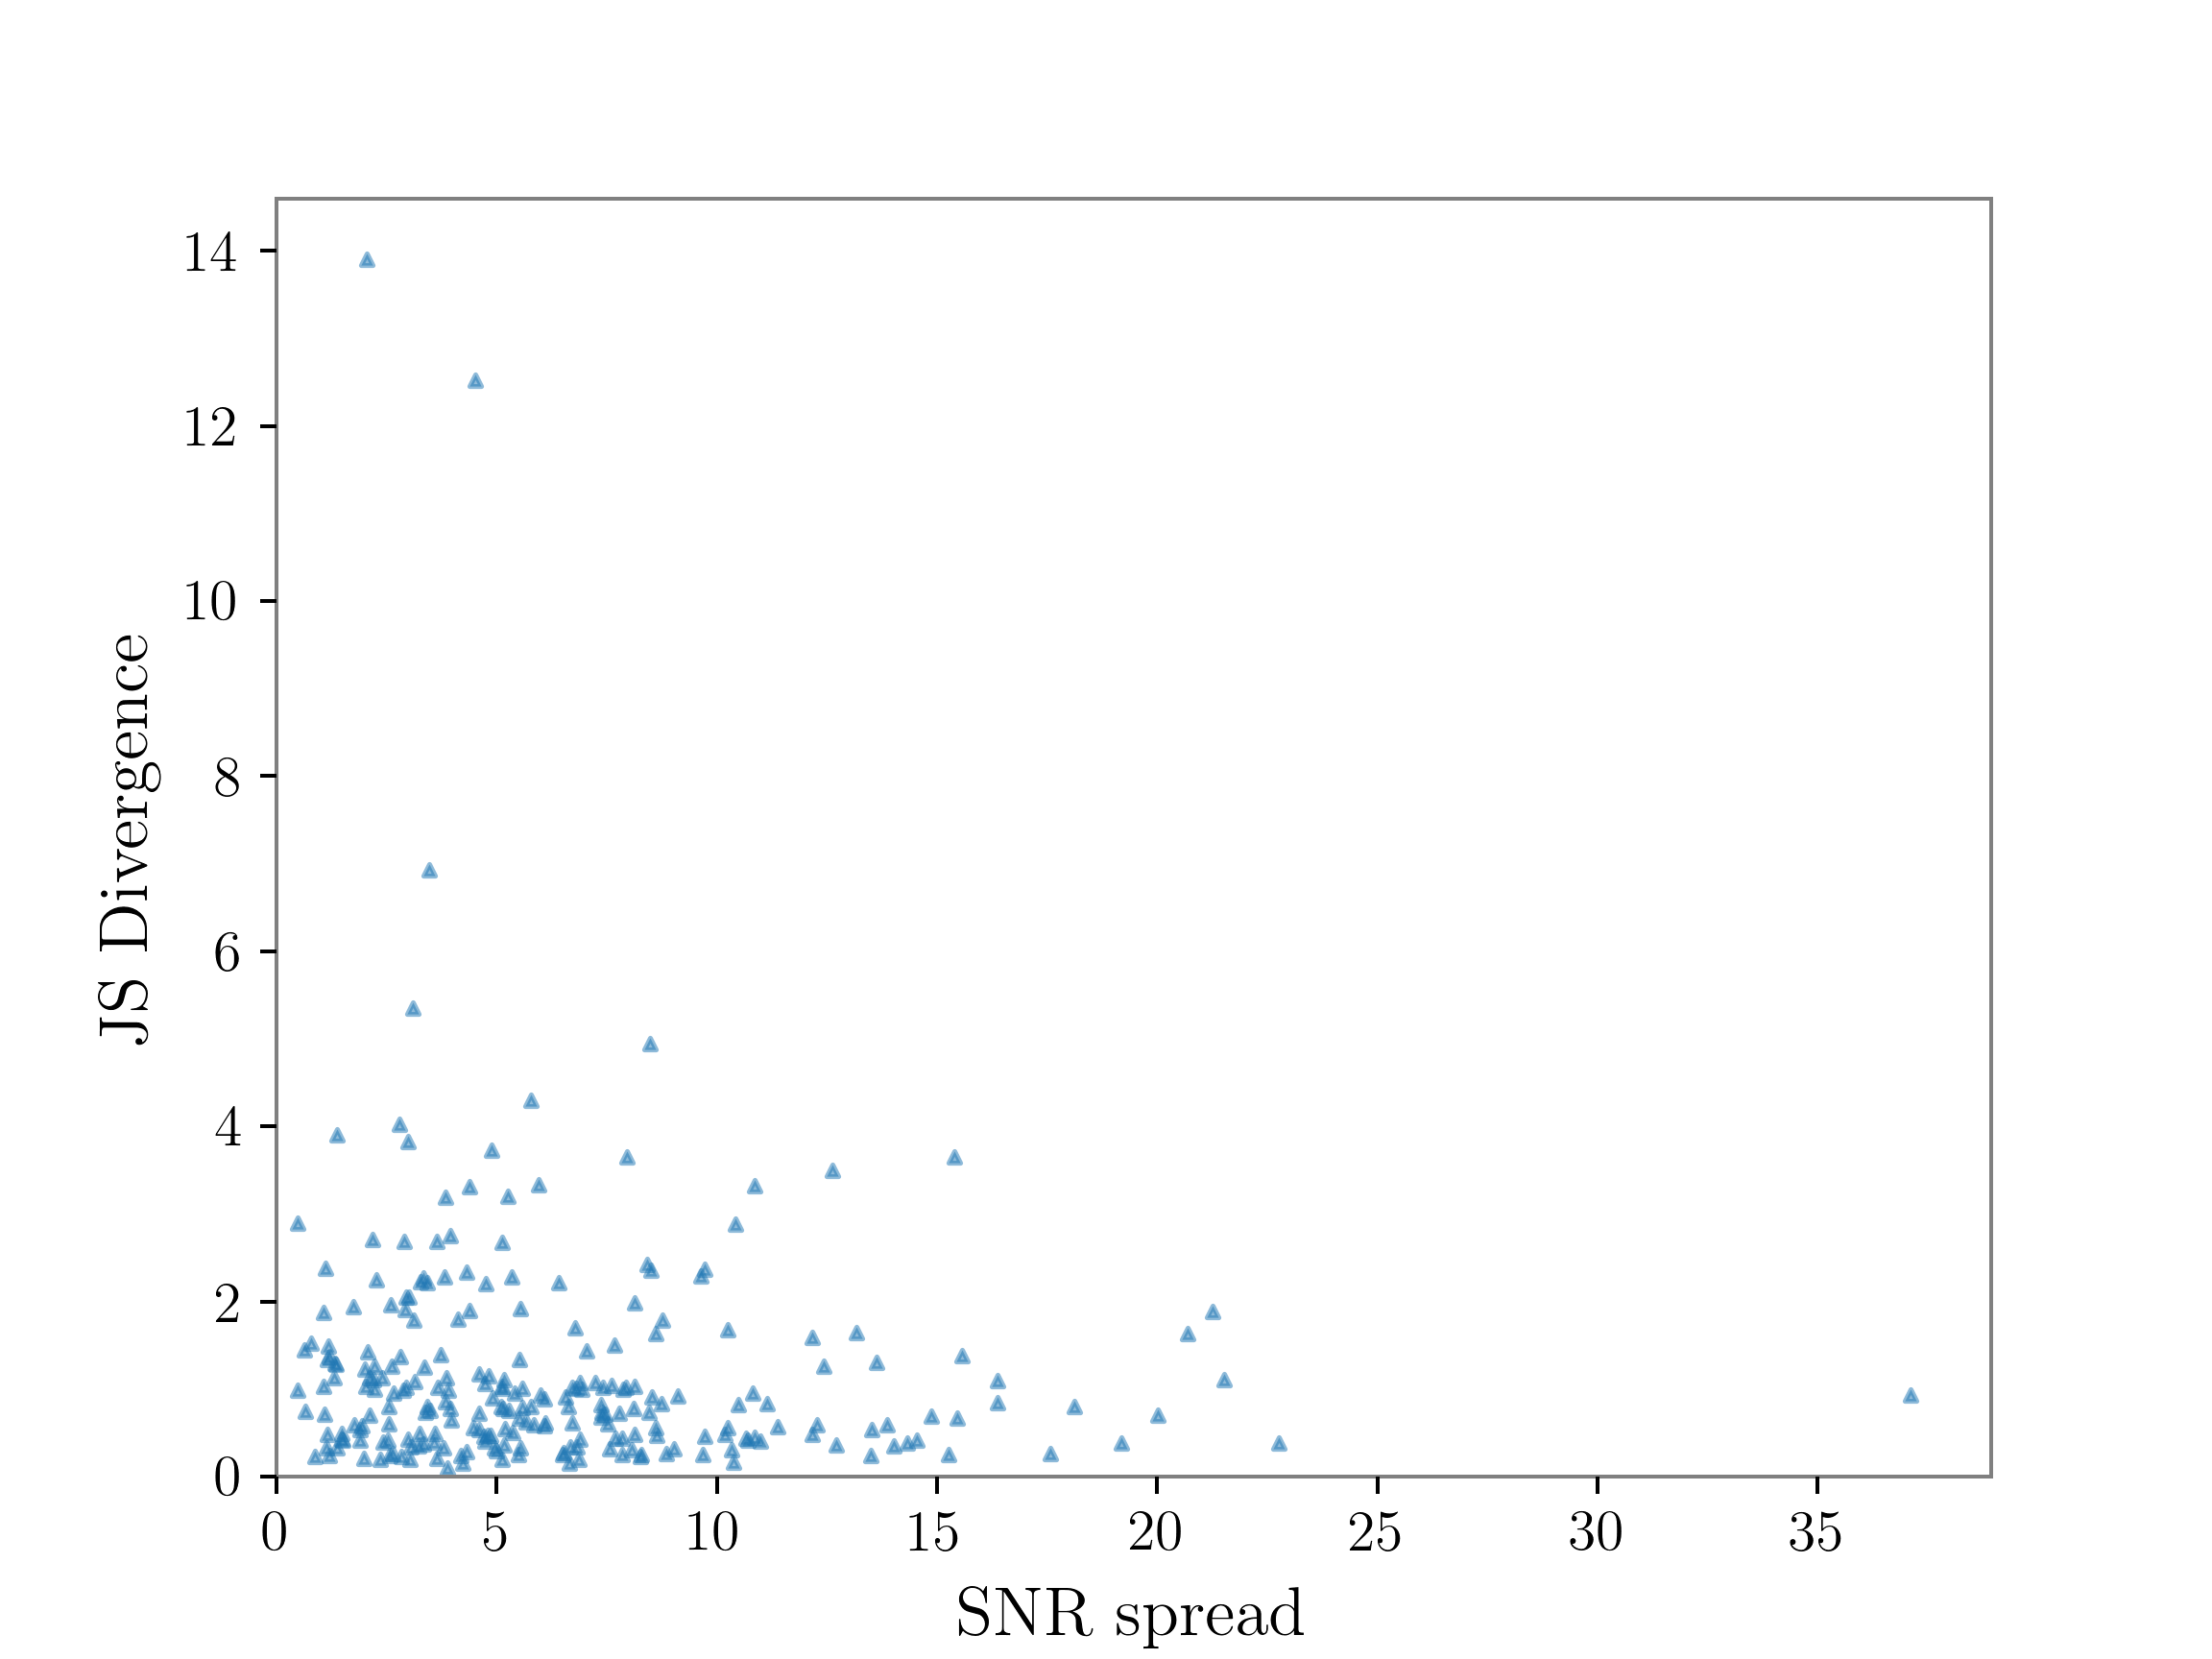
\includegraphics{figures/JS_vs_SNR-spread.png}
    \caption[14-dimensional JS-divergences of \texttt{Dynesty} vs. \texttt{VItamin} as a function of individual detector optimal SNR spread.]{\label{fig:JS_vs_SNR_dynesty} We show here 14-dimensional 
    \ac{JS}-divergence values of \texttt{Dynesty} vs. \texttt{VItamin} as a function of optimal
    \ac{SNR} (Ch.~\ref{ch:chap_1}, Sec.~\ref{sec:matched_filtering}) spread. Each triangle symbol represents a different test \ac{GW} case.}
    \label{fig:14D_JS_SNR-spread}
\end{figure}


~\chris{I also think that you should make a plot of JS divergences for the 1D cases and see if any particular parameter performs better or worse as a function of SNR. You have all the data - it's just a question of carefully choosing how to plot it and writing about it.}

\chris{Also, with the 14D JS values (and even the 1D) you should also look at the total network SNR AND look at the JS as a function of the spread in SNR - do we do worse when 1 detector doesn't see the signal?}

\subsection{VItamin Latent Space Analysis}
%
% Subsection intro
%
In this section we will introduce diagnostic plots we have used in order to gauge the behaviour of our neural network model with respect to the latent space.
%
% Discuss the corner plot for test case 184.
%
For context, we will first examine a test case at a median network 
\ac{SNR} value of \hunter{value}. As seen in Fig.~\ref{fig:comp_post_0}, this 
median \ac{SNR} event exhibits complex multi-modal behavior on multiple 
parameters including: the polarisation angle, time of coalescence, right 
ascencsion and declination. We will discuss in the following paragraphs the 
latent space structure associated with this test sample.

%
% Test set sample 0 corner plot
%
\begin{figure}
    \includegraphics[width=\columnwidth]{figures/comp_posterior_pub_plot_event_241.png}
    \caption[Posterior predictions from \texttt{VItamin}, \texttt{Dynesty} and \texttt{Ptemcee} for the median SNR test sample case in the \texttt{VItamin} paper training set.]{\label{fig:comp_post_0} Corner plot showing 2 and 1-dimensional marginalised posterior distributions for the median \ac{SNR} test dataset sample. Filled (red) contours represent the posteriors obtained from the \ac{CVAE} approach and solid (blue) contours are the posteriors output from our baseline analysis (\texttt{Bilby} using the \texttt{Dynesty} sampler). In each case, the contour boundaries enclose $68,90$ and $95\%$ probability. One dimensional marginalised posteriors for each parameter from both methods are plotted along the diagonal. Blue and red vertical lines represent the $5$---$95\%$ symmetric confidence bounds for \texttt{Bilby} and variational inference respectively. Orange crosses and vertical orange lines denote the true parameter values of the simulated signal. The original whitened noisy timeseries $y$ and the noise-free signal are plotted in blue and cyan respectively in the upper right hand panel. The test signal was simulated with network optimal signal-to-noise ratio of $10.89$.}
\end{figure}

%
% Discuss the latent space corner plots
%

There is no hard and fast rule for determining the number of latent 
space dimensions to use when deciding on the architecture for a \ac{CVAE}. 
That being said, our primary logical motivation for choosing a latent 
space size of 15 is directly related to the total number of source 
parameters we are trying to get the neural network model to learn. 
We want to ensure that the information in each source parameter dimension 
can be encoded in a latent space which is of sufficient size to do so. 
As can be seen in Fig.~\ref{fig:latent_corner_0}, there are 
some indications that this hypothesis may indeed be holding true. 

%
% Test sample 0 latent space samples corner plot
%
\begin{figure}
    \includegraphics[width=\columnwidth]{figures/latent_pub_plot_event_241.png}
    \caption[Latent space samples corner plot for a test sample in the \texttt{VItamin} paper training set.]{\label{fig:latent_corner_0} We show in this figure latent space samples from all latent space dimensions of both the $q$ encoder network (blue) and the $r_1$ encoder network (red). Each point is representative of the predicted mean values for each latent space dimension (15). Each dimension on the horizontal and vertical axis represents a different latent space dimension. 1-dimensional histograms of latent space samples for each dimension are plotted along the diagonal. Contours represent the $68, 90, 95\%$ credibility intervals.}
\end{figure}

In Fig.~\ref{fig:latent_corner_0} we plot latent space samples drawn from 
latent space predictions made by both the $q$ (blue) and $r_1$ (red) 
encoder networks after training. The probability distributions modeled by 
the encoder networks are multivariate Gaussians, whose means and 
standard deviations 
are infered by the encoders. If a dimension of the latent space is 
being used, we would expect that the corresponding 1-dimensional
marginalised posteriior for that latent space dimension along the diagonal 
of the corner plot to show some level of disagreement between the 
predictions from both encoder networks. The reasoning behind this 
statement is that the $q$ network is given a different level of 
information with respect to the $r_1$ network. Specifically, the 
$q$ network is given not only the \ac{GW} timeseries, but also the true 
values of the source parameters themselves, whereas the $r_1$ network 
is given the \ac{GW} time series by itself. If a latent space dimension 
is not being used it means that there is no additional amount of 
information that can be gleamed from that dimension, so both encoder 
networks will simply return their default, mean zero unit variate 
Gaussian distributions, which contribute nothing to the loss function. 
If nothing is being contributed to the loss function, then nothing is 
being learned from that latent space dimension. We can say that there is a 
null contribution to the loss function because the \ac{KL} divergence 
between two Gaussian distributions is known to be zero. Since the 
\ac{KL} component of the loss is zero for this dimension, weights will 
not be updated during the backpropagation process which encourage this 
dimension to be used.~\chris{OK, but lacking in mathematical rigour. We need to go through the maths in our next meeting. Each of your statements is basically correct but should be interspersed with equations supporting these statements.} 

%
% Latent dimension corner description
%
From Fig.~\ref{fig:latent_corner_0} we see that 5 of the 15 latent 
space dimensions are not being used for this test case, where the  
5 not being used from left to right on the horizontal axis are 
dimensions $z_3$,$z_4$,$z_8$,$z_{10}$, and $z_{15}$. It also appears that the $r_1$ encoder 
network (red) is in-fact choosing to produce latent space samples 
which are representative of multi-modal distributions on some dimensions ($z_2$,$z_{14}$). 
This should not be 
surprising given that the $r_1$ encoder network's final output 
latent space distributions are generated using a Gaussian Mixture 
model, where the motivation for using the Gaussian mixture model 
was to encourage the $r_1$ network to encode different modes from the posterior 
directly in the latent space. It is also evident from the 2D posterior panels (i.e. $z_1$ vs. $z_{4}$)
that the mixture model in the $r_1$ encoder network is allowing for far more 
expressive non-Gaussian shaped uni-modal distributions.
\hunter{Could add something about how phi and psi are unimodal, which is 
why only 2 dimensions have mulit-modes.}

%
% mode weight plot descriptions
%
We see show in Fig.~\ref{fig:latent_weight_0} predicted 
weights from the $r_1$ encoder network for the median \ac{SNR} 
test sample. It can be seen that the $r_1$ encoder network has assigned 
a measurable amount of likelihood to 16 out of the 32 available latent space 
modes, with all other 
modes having essentially zero weight. The fact that there are 
several modes which 
are not assigned any weight at all may 
indicate that the Gaussian mixture model in the $r_1$ encoder network could 
have a higher level of capacity than what is be needed.~\chris{I would also recommend expanding this discussion of the weights to address the ensemble behaviour as well. Maybe you cold plot all other 249 weight distributions in the background with some transparency. You could then talk about the fact that some modes are never used by any test case indicating that we have enough modes. The plot can be quite messy but if the single test case you are interested in is plotted clearly in bold then it should be fine.}. 

%
% mode corner plot posterior description
%
The effect that the integrated 
Gaussian mixture model in the $r_1$ network has on final posterior 
samples, is perhaps most clearly illustrated in
Fig.~\ref{fig:mode_corner_0}. 
Here, we sample from the 4 most likely latent space modes predicted by 
the $r_1$ encoder (colored from highest to lowest likelihood as blue, 
orange, green and red), where ``most likely'' is quantified through 
the Gaussian mixture model weights. Posteriors for each mode are 
produced by using latent samples from each mode and passing them 
through the $r_2$ decoder network. What we are left with are 
posteriors which represent the degree to which individual 
modes in the \texttt{VItamin} latent space contribute to the 
final posterior product. We note that the weight associated with 
probability of drawing a sample from each mode is not included in 
Fig.~\ref{fig:mode_corner_0}.~\chris{The only issue is the weight 
which isn't being applied in the plot. I think you should try to apply it.}. 
We see in Fig.~\ref{fig:mode_corner_0}, that the 2 most likely modes 
(blue, orange) agree strongly with each other across most 
dimensions ($\Theta_{jn}$ and $\phi_{jl}$ being possible 
exceptions), while the least likely 2 (green,red) also strong 
disagreement on some parameters ($t_0$, $\psi$, $\alpha$, $\delta$). 
One might point out that the $r_1$ network has 
not chosen to represent each mode in the posterior on $\psi$ using 
distinct modes in the latent space. We note that this is in-fact not 
surprising given that we apply a reparameterisation to the 
$\psi$ and $\phi_0$ parameters (Sec.~\ref{sec:phipsi_repar}) such that 
the number of modes the network actually ``sees'' is effectively reduced.

%~\chris{OK, we have a number of issues here - even in this case the mixture modal is identifying 2 components of the sky posterior. These are not truly separate modes because they overlap but you can just see from Fig 5.13 (the physical posterior plot) that the sky posterior is a slightly odd shape. The network has tasked 2 latent space modes to try to model this. If you then look at the 2D posteriors you can see some evidence that each mode has slightly different properties in other parameters - e.g. the blue mode prefers smaller distances compared to the yellow mode. As mentioned before it would also be good to actually weight the different coloured posteriors in the mode plot.} 

%However, because the only mulitmodal 
%components of the posterior in this test case are in the 
%polarisation angle, it's likely we do not see multimodal behaviour 
%in the latent space because of the phase-polarisation reparametersation 
%outlined in Sec.~\ref{sec:phipsi_repar}. The phase-polarisation 
%reparameterisation turns those 2 modes into 1 mode.

%
% Test sample 0 weights histogram
%
\begin{figure}
    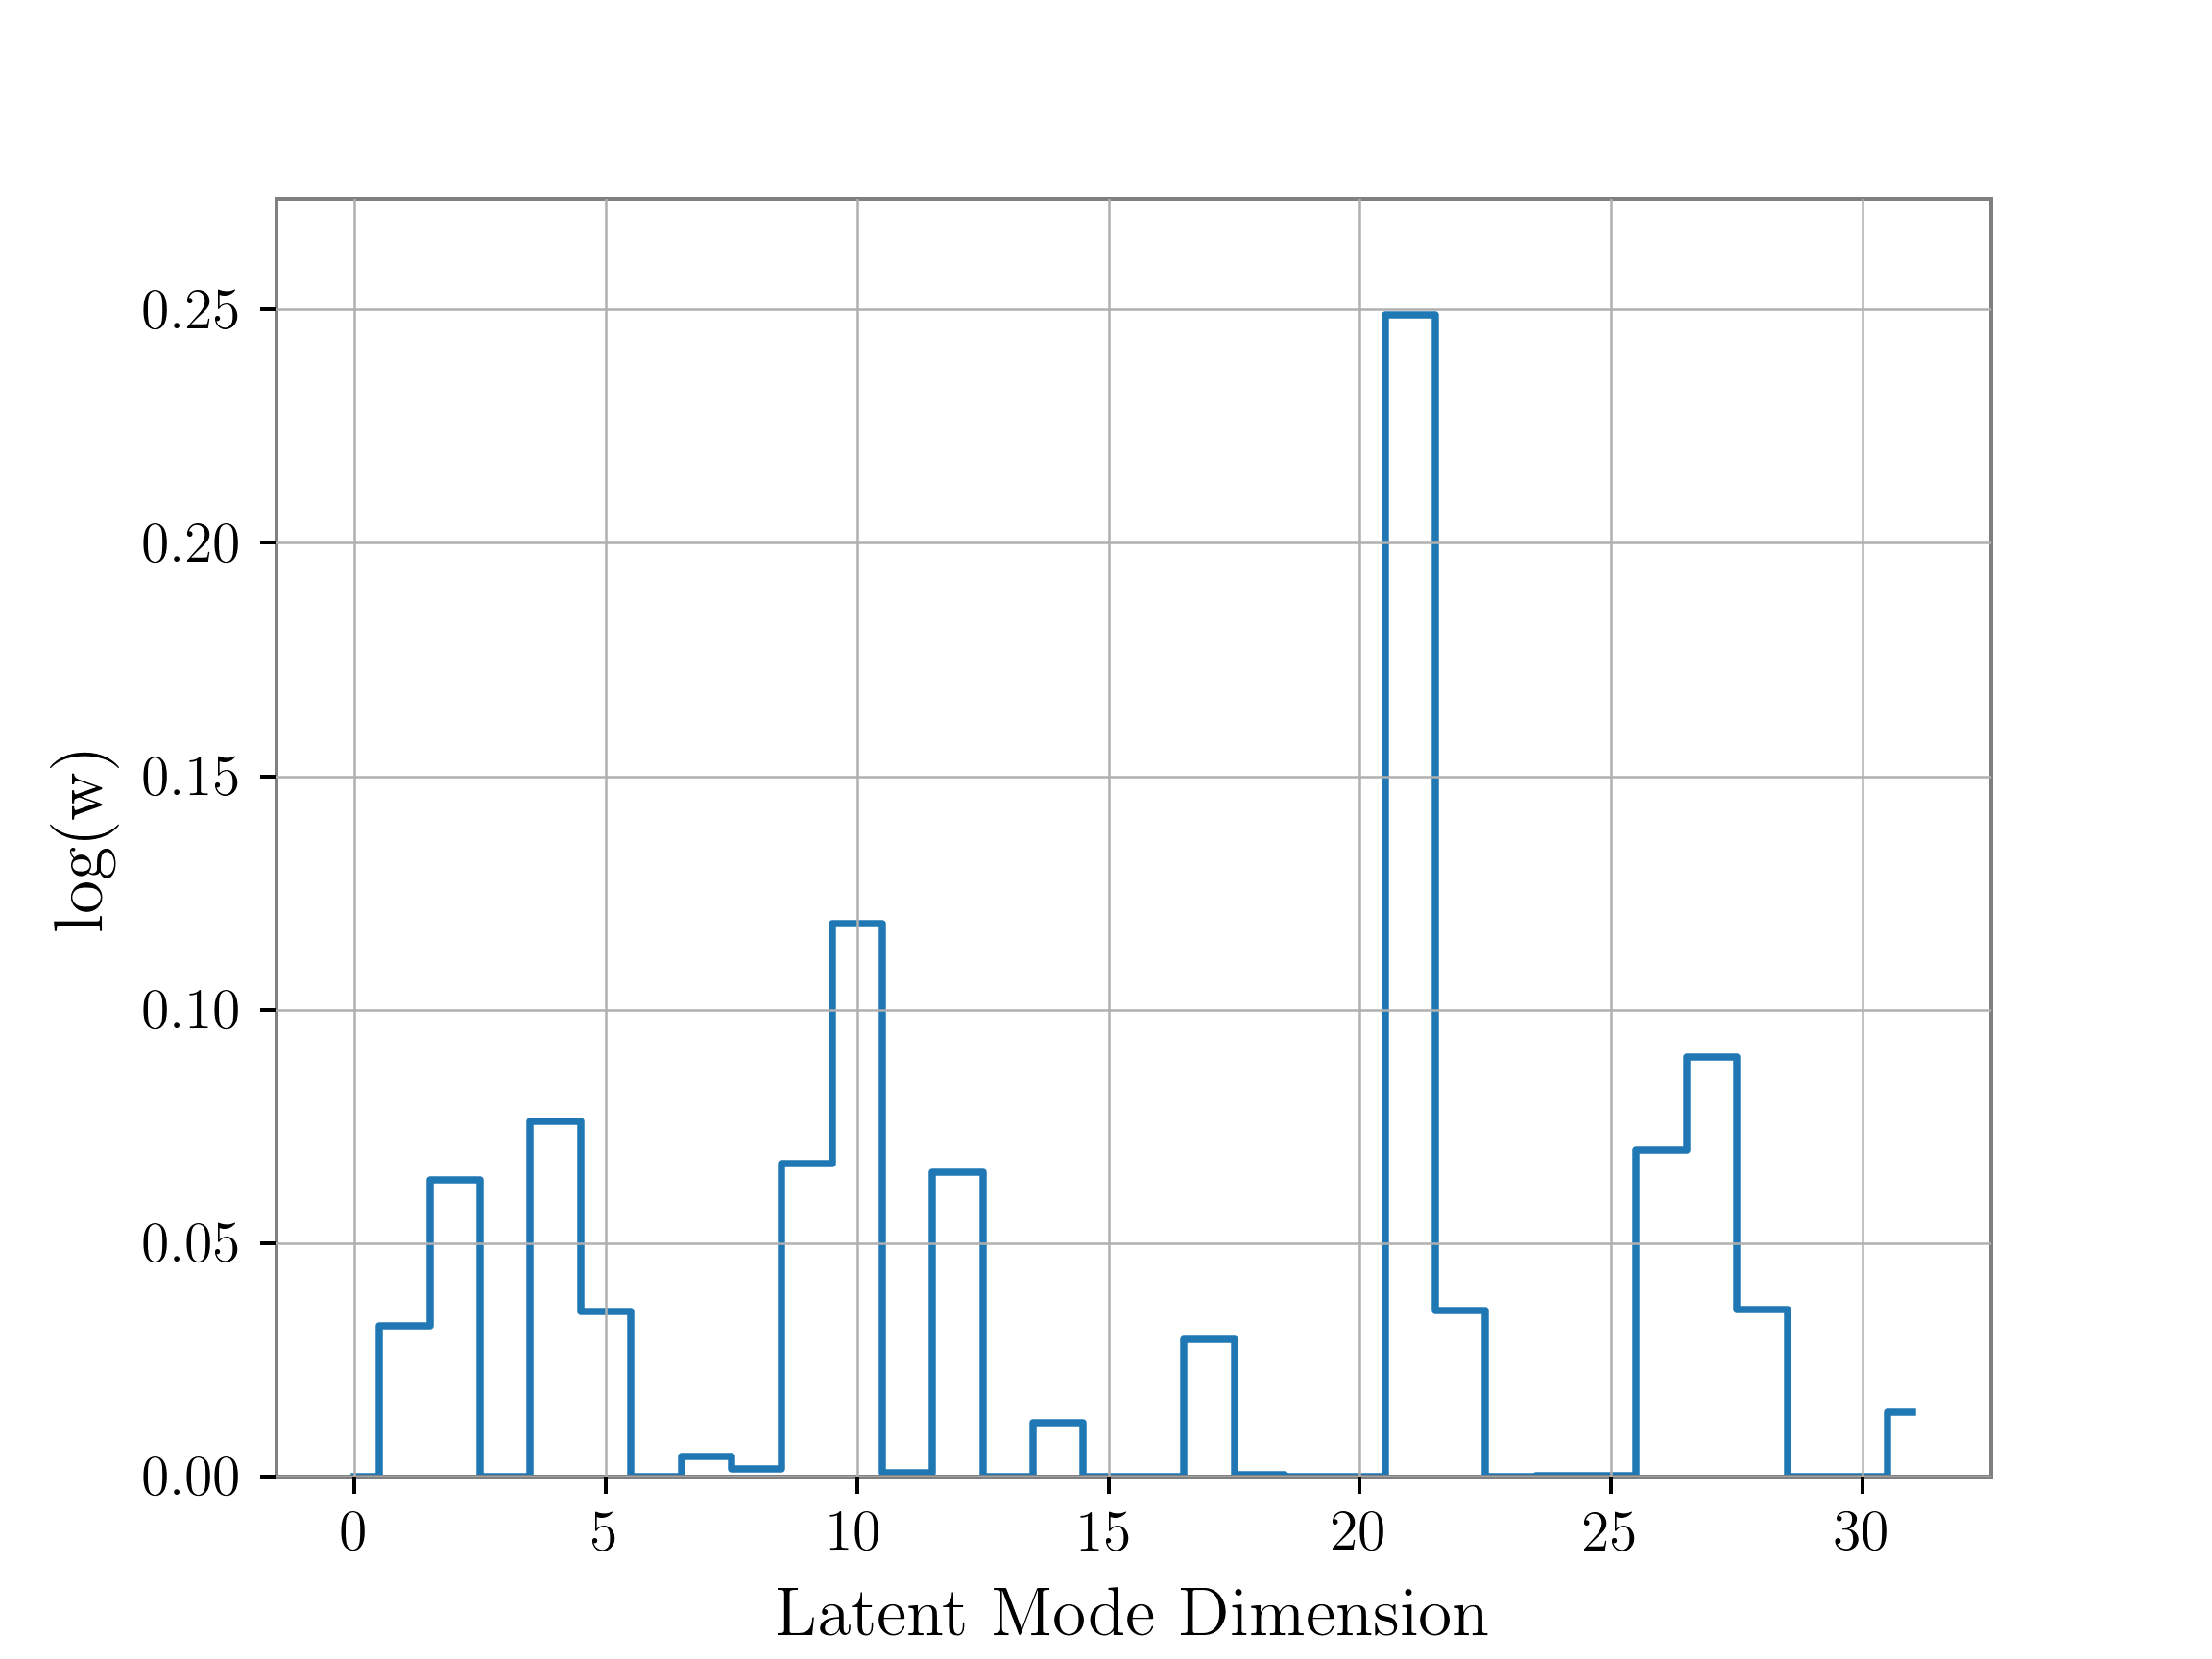
\includegraphics[width=\columnwidth]{figures/latent_weight_pub_plot_event_241.png}
    \caption[Latent space weight plot for the median SNR test sample in 
    the \texttt{VItamin} paper training set.]{\label{fig:latent_weight_0} 
    Plotted are the predicted weight values from the $r_1$ encoder 
    network for a given posterior sample of the median \ac{SNR} test 
    case as a function of latent space mode dimension number. Each 
    value is normalised such that the sum of the weights is 1, where 1 
    is representative of the network model assigning a high 
    likelihood of sampling from that particular mode. 
    \hunter{x axis should be mode number, not z dimension.}~\chris{As mentioned in the text, I recommend also plotting (with transparency) the other 249 test case weights. Keep the primary curves bold and clear to see but then you can also discuss the distribution of weights over the test cases.}}
\end{figure}

%
% Test sample 0 mode posteriors
%
\begin{figure}
    \includegraphics[width=\columnwidth]{figures/modes_posterior_epoch_pub_plot_event_241.png}
    \caption[Modal posterior corner plot for the 1st~\chris{change the test sample} test sample in the \texttt{VItamin} paper training set.]{\label{fig:mode_corner_0} Shown are posterior samples drawn from the 4 most likely latent space modes predicted by the $r_1$ encoder network. Colors denote each mode from highest to lowest mean mode weight as blue, orange, green and red respectively~\chris{you need to either state the actual weights of each mode OR even better, normalise each posterior by its weight.}. The weight associated with each mode is not accounted for in the plot. Each dimension on the $x$ and $y$ axis represents 15 source parameter posteriors predicted. 1-dimensional marginalised posteriors of posterior samples for each source parameter are plotted along the diagonal. Contours represent the $68, 90, 95\%$ credibility intervals. The orange vertical and and cross hairs represent the true source parameter values.~\chris{ make the sky plot (for each of the modes).}}
\end{figure}

What the results from Fig.~\ref{fig:mode_corner_0} may imply 
is that the multi-modality clearly seen 
in the final posteriors of Fig.~\ref{fig:comp_post_0} is being encoded across 
several modes in the latent space produced by $r_1$ encoder network. This 
could indicate that the $r_1$ encoder network
is partially determining what level of likelihood to assign to each 
mode in the posterior space. More work could be done in future 
studies to more rigorously quantify this.

%
% Test sample 184 log weights histogram
%
%\begin{figure}
%    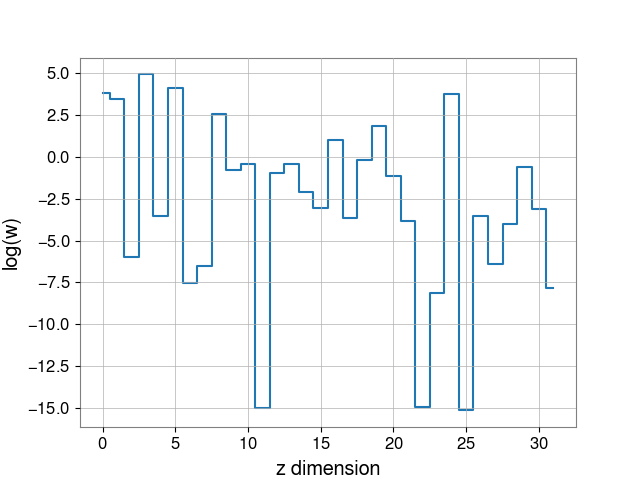
\includegraphics[width=\columnwidth]{figures/latent_logweight_pub_plot_event_184.png}
%    \caption[Latent space log weight plot for the 184th test sample in the \texttt{VItamin} paper training set.]{\label{fig:log_weight_184} Plotted are the predicted log'd weight values for the zeroth posterior sample of the 184th test sample as a function of mode latent space dimension number. Mode weights are predicted for each posterior sample by the $r_1$ encoder network.}
%\end{figure}


%%%%%%%%%%%%%%%%%%%%%%%%%%%%%%%%%%%%%%%%%%%%%%%%%%%%%%%%%%%%%%%%%%
%%%%%%%%%%%%%%%%%%%%%%%%%%%%%%%%%%%%%%%%%%%%%%%%%%%%%%%%%%%%%%%%%%
%%%%%%%%%%%%%%%%%%%%%%%%%%%%%%%%%%%%%%%%%%%%%%%%%%%%%%%%%%%%%%%%%%
\subsection{Dynesty vs. Dynesty Jensen--Shannon Divergence}\label{dyn_v_dyn_JS}

Here we provide some discussion regarding the lower limit of \ac{JS} values 
we might expect from \texttt{VItamin}. We approximate a rough 
limit by comparing two 
independent \texttt{Dynesty} runs on all $250$ test sample cases 
for both the full 14-dimensional \ac{JS}-divergence and the 1-dimensional 
\ac{JS}-divergence.

%
% Discuss dynesty vs. dynesty on the full 14D case
%
In Fig.~\ref{fig:dyn_vs_dyn_ful14D_JS}, we compute the \ac{JS}-divergence 
between two independent runs of \texttt{Dynesty} for 
each of the 250 test cases across all 14 dimensions. The mean 
\ac{JS} value across all test cases is $0.05$ with tails extending to a 
lower bound of $\sim 10^{-3}$~\chris{if this is for the 14-D case 
then I'm sceptical of the lower bound here - I know that the
universal divergence code gives negative numbers sometimes. You need to show and discuss the limitations and settings that you used to get these numbers.} and 
an upper bound of $\sim 10^0$. Given that the \texttt{Dynesty} sampler 
is known within the \ac{GW} parameter estimation community to be one of the most
trusted and reviewed samplers~\cite{2010.14527}. Given that \texttt{Dynesty} 
is generally consistent between runs of the same data, we would expect 
that two independent runs of the \texttt{Dynesty} sampler should 
provide us with a reliable lower limit on the best expected 
\ac{JS} values we could hope to achieve. Given the range of 
\ac{JS} values seen in Fig.~\ref{fig:dyn_vs_dyn_ful14D_JS} and 
comparing those values to those of Fig.~\ref{fig:kl_results}, we see 
that \texttt{VItamin} results plotted against other sampler results do 
generally seem to have larger \ac{JS} values than the mean of 
$0.05$ seen in Fig. \ref{fig:dyn_vs_dyn_ful14D_JS}. This is to be 
expected though because the \ac{JS} values shown 
in  Fig.~\ref{fig:dyn_vs_dyn_ful14D_JS} 
indicate a lower bound on the level of disagreement we 
expect \texttt{VItamin} to achieve between other 
sampler approaches. Furthermore, we see that the lowest \ac{JS} value tails
over all comparison results of 
Fig.~\ref{fig:kl_results} are consistent with the tails 
of Fig.~\ref{fig:dyn_vs_dyn_ful14D_JS}. 
~\chris{the plot you refer to here is rather dull. Why not also plot the equivalent distributions for the other samplers (including vitamin) as well?}

%
% Dynesty vs. Dynesty Full JS
%

\begin{figure}
    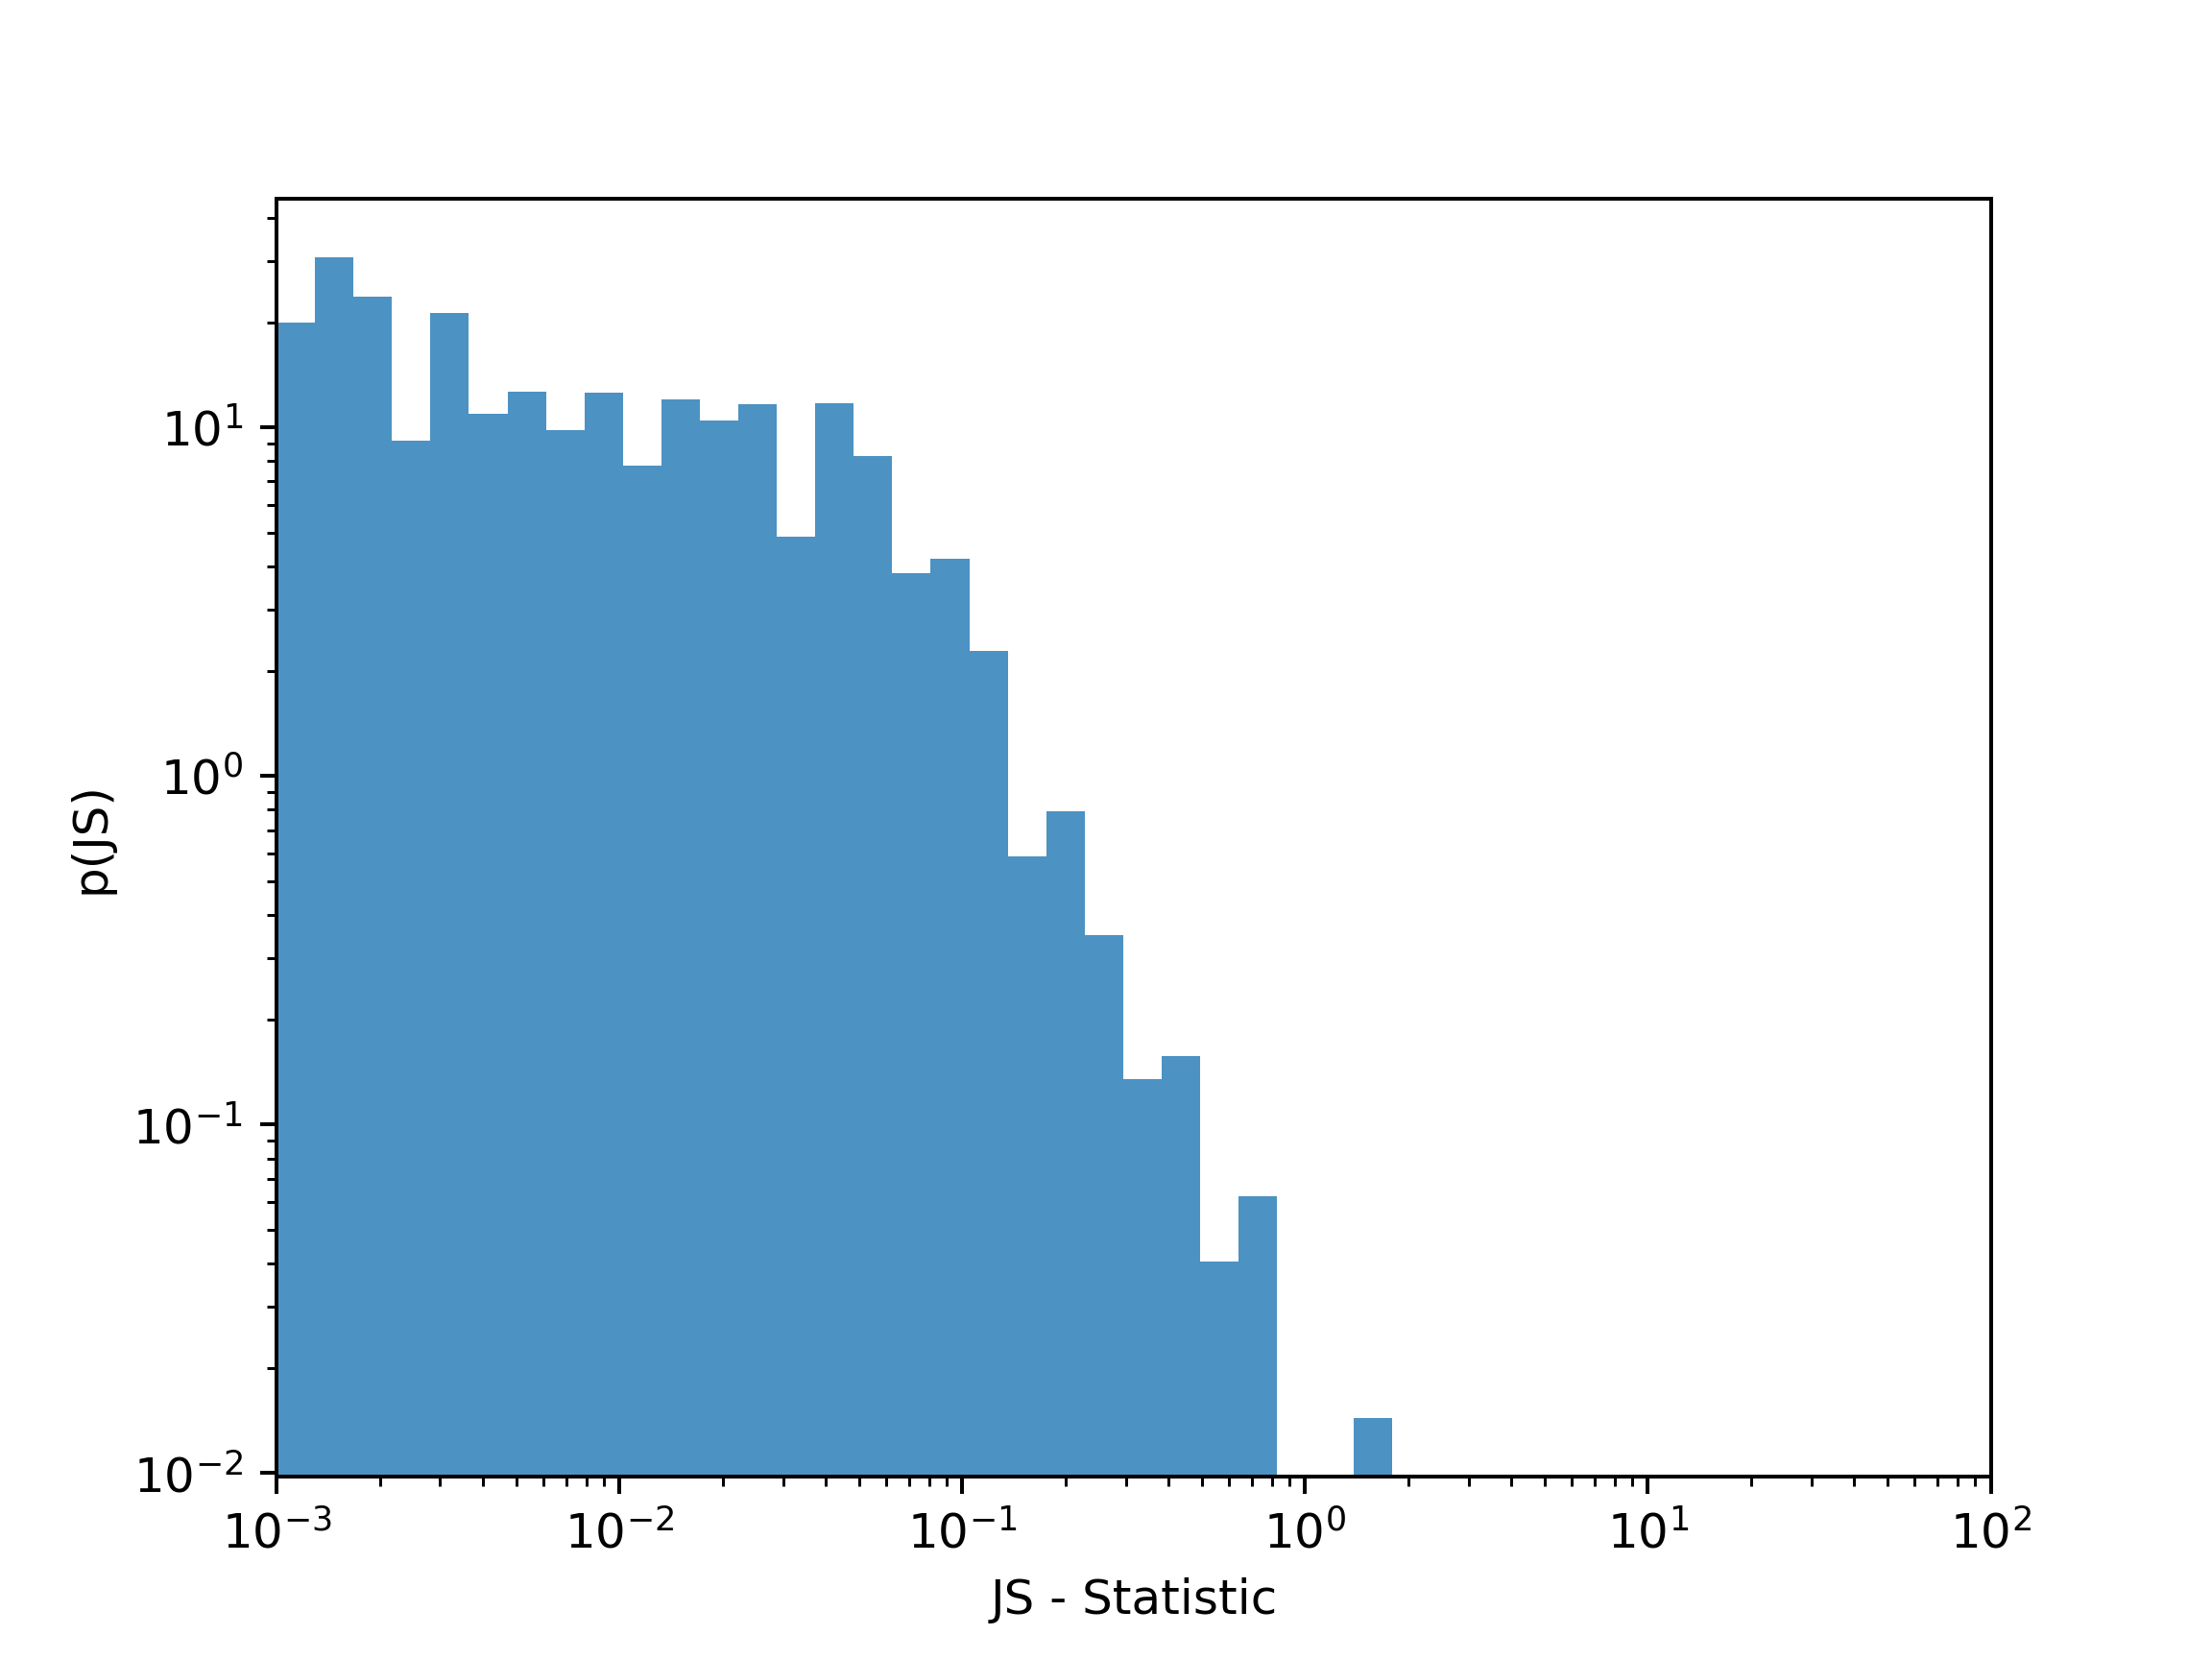
\includegraphics[width=\columnwidth]{figures/dynesty-dynesty_fullJS.png}
    \caption[\texttt{Dynesty} vs. \texttt{Dynesty} 14-dimensional \ac{JS} divergence probability distribution plot.]{\label{fig:dyn_vs_dyn_ful14D_JS} A probability distribution of \ac{JS}-divergence values for \texttt{Dynesty} vs. another independent run of \texttt{Dynesty} using 14-dimensional 
    posteriors on the same test data. The mean \ac{JS} divergence has a value of $0.05$~\chris{indicate this on the plot visually}. We note that since since the \ac{JS}-statistic is calculated using the \texttt{universal-divergence}~\cite{4839047} code-base, that there are some negative values which are not shown here.~\chris{this should also be mentioned and explained in the main text. Also, as mentioned before, to make this more interesting you could also plot the same curves for the other samplers here too. Finally, can you sort out the fonts so that this is the same as the other plots and add (nats) to the x-axis label.}}
\end{figure}

%
% Dynesty vs. Dynesty 1D JS
%
In Fig.~\ref{fig:dyn_vs_dyn_indi_JS} we plot the \ac{JS}-divergence 
between independent \texttt{Dynesty} runs for using 
1-dimensional marginalised source parameter posterior results. Instead of 
using the \texttt{universal-divergence} code, we
calculate the \ac{JS}-divergence using the analytic expression 
defined in Eq.~\ref{eq:JS_div} on the 1-dimensional marginalised posteriors 
between the two \texttt{Dynesty} runs.~\hunter{not sure if it's worth it 
to repeat the uncertainties here.} In the figure, different colors 
represent different source parameter \ac{JS} distributions over all 
250 test cases. We see 
that \ac{JS}-diverence values across all source parameter distributions 
range from $\sim1 \times 10^{-4} - 10^{-1}$. 
The mean 1-dimensional \ac{JS} value across all source parameter distributions
is 
approximately $\sim 10^{-3}$. This value indicates a lower limit 
on the \ac{JS}-divergence values we would expect to see with respect to 
comparison results using 1-dimensional marginalised posteriors. 
\hunter{Is this more coherent now?}

\begin{figure}
    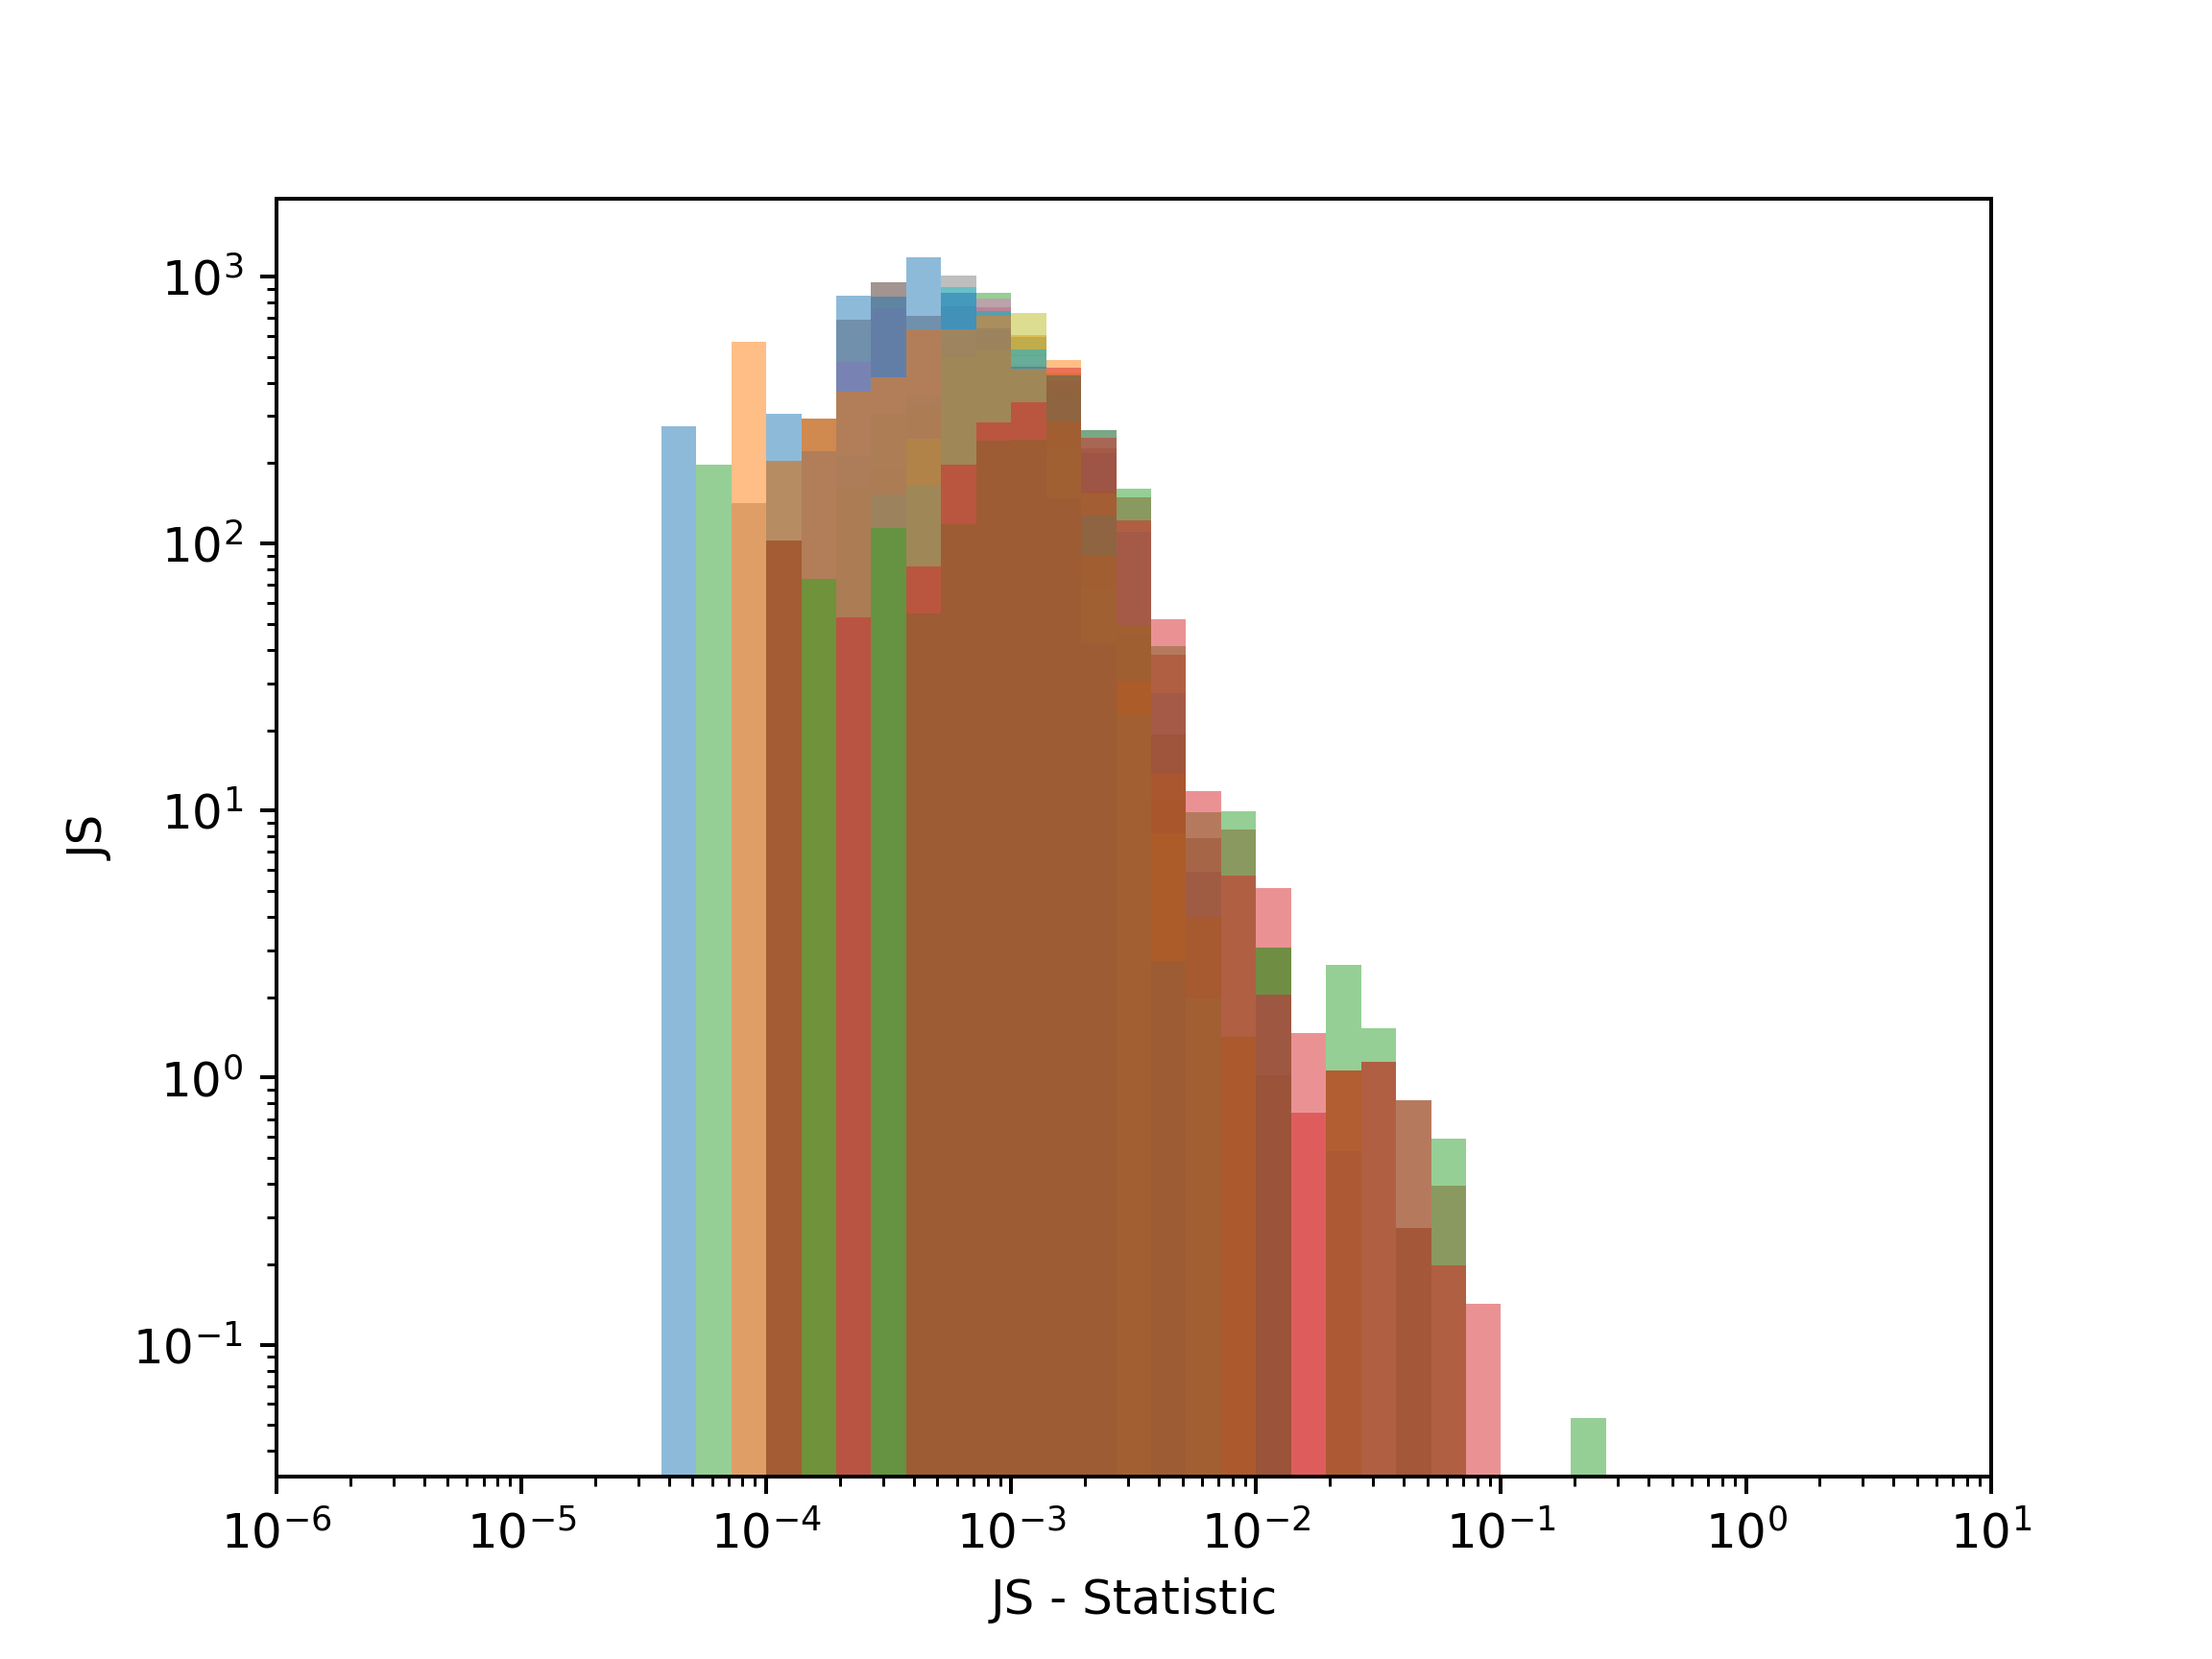
\includegraphics[width=\columnwidth]{figures/dynesty-dynesty_indiJS.png}
    \caption[Dynesty vs. Dynesty full 1-D JS divergence histogram plot.]{\label{fig:dyn_vs_dyn_indi_JS} Shown are histograms of 1-dimensional JS divergence values for \texttt{Dynesty} vs. another independent run of \texttt{Dynesty}. Different colors represent JS values with respect to individual source parameter posterior \texttt{Dynesty} predictions. Mean JS values for each source parameter are given as: $m_1 \sim 0.00139$, $m_2 \sim 0.00143$, $d_l \sim 0.00142$, $t_0 \sim 0.00358$, $\theta_{jn} \sim 0.00192$, $\psi \sim 0.00134$, $a_1 \sim 0.00101$, $a_2 \sim 0.00088$, $\Theta_1 \sim 0.00143$, $\Theta_2 \sim 0.00123$, $\phi_{12} \sim 0.00080$, $\phi_{jl} \sim 0.00136$, $\alpha \sim 0.00538$, $\delta \sim 0.00401$. JS values are calculated using the \texttt{scipy} JS divergence code-base.~\chris{I like what you're trying to do here but I think this would be far better displayed using box plots - you are currently struggling to represent the means using the caption which is not very sensible. With box plots you can still show the distribution but also then see how different parameters behave. I think this would be very useful and warrant discussion since I might expect some parameters to potentially have larger fundamental JS-calculation errors than others.}}
\end{figure}

%%%%%%%%%%%%%%%%%%%%%%%%%%%%%%%%%%%%%%%%%%%%%%%%%%%%%%%%%%%%%%%%%%
%%%%%%%%%%%%%%%%%%%%%%%%%%%%%%%%%%%%%%%%%%%%%%%%%%%%%%%%%%%%%%%%%%
%%%%%%%%%%%%%%%%%%%%%%%%%%%%%%%%%%%%%%%%%%%%%%%%%%%%%%%%%%%%%%%%%%
\section{Data Augmentation and Normalisation}\label{sec:vit_data_aug}

As discussed previously in in Ch.~\ref{ch:chap_2}, it is 
oftentimes advantageous to augment the training set during training 
of a neural network. This is done to decrease the complexity of 
the search space, as well as to provide a greater variety of 
signals to the network such that it is better able to generalise 
to new signals when testing the model. 

%
% Normalisation
%
The first and most simple augmentation method we employ is that of
normalisation. 
We normalise each source parameter value for all training samples such that 
they lie between the values of zero and one (i.e. on the unit-hypercube). We also normalise the 
all timeseries in the training set using a normalisation factor such that all  
timeseries values also lie on the 
range from zero to one. We note that this timeseries normalisation factor 
must also then be applied during testing when using a pre-trained neural network. 
Both of these normalisations are performed in order to reduce the search 
space complexity. 

%
% hour angle sky conversion stuff
%
We also convert the right ascension source parameter values to 
the hour angle parameter space. This is done because due to the 
definition of right ascension whereby different \ac{GPS} times 
will correspond~\hunter{Need to ask Chris why hour angle conversion is 
done again.}

%
% 2D cyclic parameter representation
%
In order to make it easier for the network to predict cyclic parameter 
values which lie on the wrapped edges of the cylcic parameter space, we 
reparameterise all cylcic parameter values to be on the abstract 
2D plane. This conversion is done by enforcing the decoder network to 
produce 2 means and 1 standard deviation characterising multivariate 
Gaussians for each cyclic parameter (as 
opposed to the 1 mean for all other source parameters). The angle 
is then computed between the 2 predicted cyclic parameter means 
through the inverse tangent function. The inverse tangent converts the 
2-dimensional representation back to the original 
parameter space for all cyclic parameters. 

~\chris{This all fits in nicely with the augmentation stuff- don't forget the hour angle sky conversion too.} Another augmentation technique that we apply 
is to 
allow the network to see multiple noise realizations of the same 
signal multiple times. This is done by first enforcing that the network 
be run over a subset of the entire training set, $2\times10^4$ unique training 
sample waveforms, $4$ times. The cost function of the network 
is calculated by drawing a 
random batch of signals from the current training subset of $2\times10^4$
signals, whereby each signal in the batch  
is assigned a new white Gaussian 
noise realisation. This means that we effectively train over an infinite 
number of Gaussian noise realisations.
After the network has seen $2\times10^4$ training signals $4$ times we then 
load in a new subset of $2\times10^4$ training signals. By giving the network 
multiple noise realisations for the same signals, we are hopefully 
encouraging the network to generalise to new noise realisations 
during testing.

%
% t0, phi, distance augmentation
%
Every time we give the network a new chunk of $2\times10^4$ signals, 
we also randomize the phase, time of arrival and distance of the 
new loaded in training samples. We note that the new chunk of signals 
is read in already having existing values which have beend drawn from 
the prior. This process is to relabel the source parameter values with 
new draws from the prior and to also modify the noise-free timeseries 
of the training samples accordingly.
%
% Distance augmentation
%
For distance, we first choose values uniformly at random from 0 to 1 for 
each distance training sample parameter. These values are then 
converted to units of Mpc by 
%
\begin{equation}\label{eq:dist_rescale}
    d_{\textrm{new}} = d_{\textrm{min}} + d_{\textrm{uni}} (d_{\textrm{max}} - d_{\textrm{min}}),
\end{equation}
%
where $d_{\textrm{uni}}$ is a uniform set of numbers between 0 and 1, 
$d_{\textrm{max}}$ represents the maximum allowed distance according to 
the prior and $d_{\textrm{min}}$ is the minimum allowed distance 
according to the prior. We sample $d_{\mathrm{uni}}$ from a unfiform 
distribution simply because that is the prior we use for the 
luminosity distance. We then determine the scale factor by which 
the distance has changed from its old value for each training 
sample by dividing the old distance by the new distance value.
%
\begin{equation}
    s = \frac{d_{\textrm{old}}}{d_{\textrm{new}}}
\end{equation}
%
where $d_{\textrm{old}}$ is the original distance value for the sample and $d_{\textrm{new}}$ is the new value. In summary, all we're doing here is drawing 
a new distance from the prior, and then computing a ratio between the old 
and new distance.

%
% Phase augmentation
%
In order to get the phase augmentation correction term we do a similar 
process as the distance augmentation above. We begin by drawing 
a new phase value from the prior with bounds that are defined by the 
phase prior. A phase correction term is then calculated
%
\begin{equation}
    \Phi_{\phi_0}^{\textrm{corr}} = -\exp\left(i(\phi_0^{\text{new}} - \phi_0^{\text{old}})\right),
\end{equation}
%
where $\Phi_{\phi_0}^{\textrm{corr}}$ is the phase correction factor we 
will use to randomize the phase, $\phi_0^{\textrm{new}}$ is the new 
randomized phase value and $\phi_0^{\textrm{old}}$ is the 
original training sample phase value.

%
% time correction
%

The time of coalescence correction term is then computed 
again by first randomly drawing a new time of coalescence from the 
prior. We then find the difference between the new and old 
times and convert to the frequency domain given by the expression 
%
\begin{equation}
    \Phi_{t_0}^{\textrm{corr}} = -\exp\left(i\,2\pi\,\vec{f_t}(t_0^{\text{new}} - t_0^{\text{old}})\right)
\end{equation}
%
\hunter{May want Chris to check this.}
where $t_0^{\textrm{new}}$ is the new time of coalescence, 
$t_0^{\textrm{old}}$ is the old time of coalescence, 
$\vec{f_t}$ is a frequency vector with values from 0 to the nyquist 
frequency, and $\Phi_{t_0}^{\textrm{corr}}$ is the time of coalescence 
correction factor.
Finally, given all the correction 
factors for time of coalescence $\Phi_{t_0}^{\textrm{corr}}$, distance $s$ and 
phase at coalescence $\Phi_{\phi_0}^{\textrm{corr}}$ have been calculated, 
we need only simply multiply the phase correction term and the 
time correction term by the real \ac{FFT}~\cite{Cooley1965AnAF} 
of the training sample 
timeseries, $y$, where we note the time correction term is 
frquency dependent and the phase correction term is a constant. 
The application of all the correction terms may be 
expressed as
%
\begin{equation}
    y_{\phi \textrm{corr}} = \mathcal{F}(y)\, \phi_{\textrm{corr}}\, t_{\textrm{corr}},
\end{equation}
%
where $\mathcal{F}$ is the \ac{FFT}. %defined as 
%
%\begin{equation}
%    \mathcal{F}(y) = \sum_{n=0}^{N-1} y(n) \exp\left(\frac{-i 2\pi k n}{N} %\right),
%\end{equation}
%
%where N is the total size of the time series, $k$ is 
We note here that the time correction term effectively ``slides'' the signal 
in time, such that the end of the signal can be slid past the end of 
the timeseries and end up at the start of the timeseries, and vice versa. 
This is obviously unphysical, but we emphasise that our signals are 
constructed so that they do not have significant amplitude at the 
boundaries of our timeseries. Additionally, the time of coalesence 
window defined by the prior is relatively narrow, hence we expect 
no unphysical signal wrapping.

%
% Get back to time domain
%
To apply the distance term we  
compute the inverse real \ac{FFT}~\cite{Cooley1965AnAF}, $\mathcal{F}^{-1}$, 
of $y_{\phi \textrm{corr}}$ and 
multiply by the distance correction scale factor
%
\begin{equation}
    y_{\phi \textrm{corr}} = \mathcal{F}^{-1}(y_{\phi \textrm{corr}})\, d_{\textrm{corr}}. 
\end{equation}
%
Adding these randomized elements to the existing training workflow may   
help to ensure that the neural network model does not 
overfit the training set. We also note that these augmentations 
were a computationally cheap and simple 
method for expanding the effective training set size.

%%%%%%%%%%%%%%%%%%%%%%%%%%%%%%%%%%%%%%%%%%%%%%%%%%%%%%%%%%%%%%%%%%
%%%%%%%%%%%%%%%%%%%%%%%%%%%%%%%%%%%%%%%%%%%%%%%%%%%%%%%%%%%%%%%%%%
%%%%%%%%%%%%%%%%%%%%%%%%%%%%%%%%%%%%%%%%%%%%%%%%%%%%%%%%%%%%%%%%%%
\section{Phase and Psi Reparameterisation }\label{sec:phipsi_repar}

One of the biggest issues we have faced while training the neural network has 
been dealing with the complex 
multi-modal nature of the phase ($\phi$) and psi ($\psi$) parameters. 
Along with the addition of the Gaussian mixture model component of the network 
mentioned previously, we have also implemented a reparameterization of both phase and 
polarisation angle in order to simplify the search space for the neural 
network partly inspired by the work of Jones in~\cite{10.1093/mnras/stv1584}.

% why we are allowed to do this.
We are allowed to make the following reparameterisation due to the degeneracies 
in $\psi$ and $\phi_0$ of the signal model we use, where degeracy refers to different 
$\psi,\phi_0$ combinations which give rise to the same \ac{GW} waveform. We note that 
if the signal contains higher order modes, these degeneracies are broken and thus 
this reparameterisation would not be applicable in that case.~\hunter{Is this 
enough of an intro to say why we're allowed to do this?}
In order to go from $\psi$ and $\phi$ to a new representation $\psi^{'}$ and $X$, 
we first take the remainder of the ratio 
$\phi_0+\psi$ and $\pi$ which then becomes a new parameter denoted as $X$ given by
%
\begin{equation}
    X = (\psi + \phi_0) \textrm{ mod } \pi,
\end{equation}
%
where ``mod'' is the modulus. We also take the remainder 
of the ratio $\psi$ and $\pi/2$ given as
%
\begin{equation}
    \psi^{'} = \psi \textrm{ mod } \frac{\pi}{2}.
\end{equation}
%
In order to get back to the original $\psi, \phi_0$ representation, we 
choose a set of two random integers with equal probability between zero and 
$2\pi$ (denoted as $D_1$), as well as a 
set of two random integers with equal probability between $0$ and $\pi/2$ (denoted as $D_2$) 
for each $\psi$ value and ensure both $\psi^{'}$ and 
$X$ are in radians.
~\chris{D1 and D2 basically define which of the 4 tessellation that we use. I would discuss the tessellation figure before explaining the reverse process.} We then subtract off $\psi^{'}$ from $X$, add both random radian integers and take the modulus  of the whole expression with respect to $2\pi$ in order to get back $\phi_0$. 
%
\begin{equation}
    \phi = ((X - \psi^{'}) + D_{1} + D_{2}) \textrm{ mod } 2\pi     
\end{equation}
%
To get back to $\psi$ we add set 
$D_2$ and take the modulus with respect to $\pi$
%
\begin{equation}
    \psi = (\psi^{'} + D_2) \textrm{ mod } \pi.
\end{equation}
%
This essentially tessellates the $X-\psi$ and $\psi$ parameters across four quadrants of the parameter space while maintaining the same number of samples and general distribution shape.~\chris{I find this explanation of how to get back to psi and phi very confusing - best to make more use of the figure with a clear description of what you're plotting and discuss it earlier on.}

The reparameterisation process is visually illustrated in Fig.~\ref{fig:Xpsi}. It can be clearly seen that the 2-dimensional representation 
$X, \psi^{'}$ in both the upper 
left and lower right subplots, is vastly simpler than the original 2D $\phi_0, \psi$ representation. 
The transformation is also able to maintain the property of being 
reversible~\chris{well, not really. What does fully mean here? The process we have does not guarantee that being transformed forward then back would put you in the same place. Forwards maps you to the single master tessellation shape but backwards equally randomly places you in one of the 4 other tesselations. So not entirely reversible.}. 
Although, we do note that if one considers \ac{GW} template waveforms with higher 
order modes this degeneracy is broken and the above reparameterization would not be necessary~\cite{10.1093/mnras/stv1584}.

~\chris{One thing we don't address is the mystery as to why the CVAE didn't model the degeneracy itself. We needn't bring this up and simply argue that the reparameterisation is natural for our problem and simply avoids us having to deal with multimodal structures in the psi-phase space. You allude to this issue in your last sentence where you say that for higher modes this reparameterisation wouldn't be necessary. However, it's more like it wouldn't be valid. Whether or not the CVAE would then work without it is an unknown. }

\begin{figure}
    \centering
    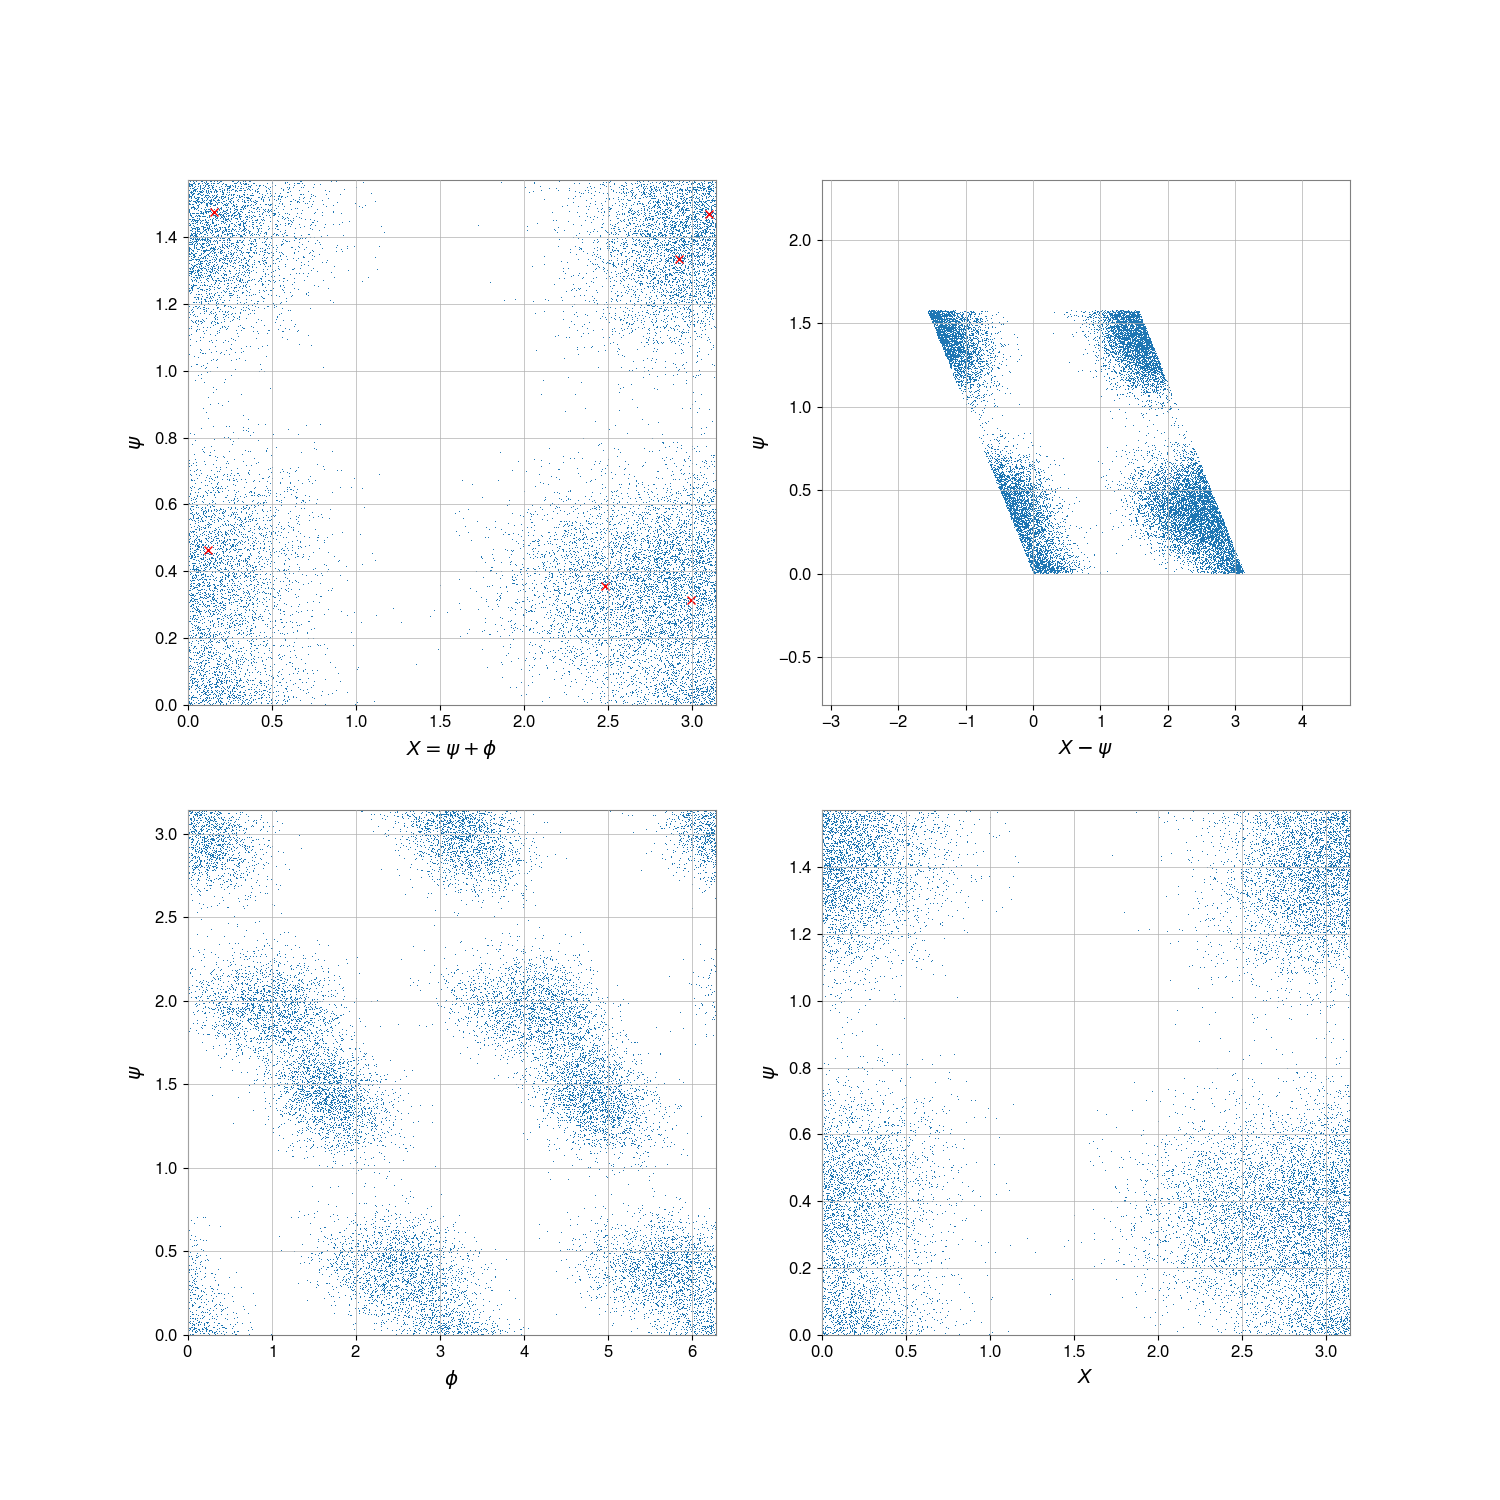
\includegraphics[width=16cm,height=20cm,keepaspectratio]{figures/Xpsi.png}
    \caption[An illustration of the $\psi$ and $\phi$ reparameterisation.]{
    An illustration of the $\psi$ and $\phi$ reparameterisation. Upper left 
    plot: a random set of samples drawn from randomly chosen 
    multi-component (mixture) Gaussians for both $\psi$ and $\phi$
    ~\chris{the top left plot is representative of a single master 
    tessellation in the psi' and X space}. Red crosses denote each 
    Gaussian's mean and $X$ represents a reparameterization of 
    $\psi$ and $\phi$. Upper right: Same plot as the upper 
    left, 
    but with $\psi$ subtracted off from the reparameterisation in 
    order to form a trapezoidal-like shape for tessellation purposes. 
    Lower left: We then apply a tessellation of the samples in the 
    upper right figure in order to convert the reparameterisation back 
    to the original units of $\psi$ and $\phi$. Lower right: We can 
    get back to the reparameterised version by applying our 
    reparameterisation trick again without any change to the original 
    in the upper left.~\chris{We need to discuss exactly what these plots represent and how they were constructed. Assuming that the "trick" is valid then we generate in the psi', X space first (top right). We convert this to the psi,phi space in the top right. We tessellate the top right plot (using your D1 and D2 randomisation) to make lower left plot showing that the distribution on the full physical psi,phi space is just copies of the top right. The lower right plot is the lower left plot converted directly into psi', X and we can see that it is identical to the original top left plot.}}
    \label{fig:Xpsi}
\end{figure}

%%%%%%%%%%%%%%%%%%%%%%%%%%%%%%%%%%%%%%%%%%%%%%%%%%%%%%%%%%%%%%%%%%%%%%
% CONCLUSIONS
%%%%%%%%%%%%%%%%%%%%%%%%%%%%%%%%%%%%%%%%%%%%%%%%%%%%%%%%%%%%%%%%%%%%%%
%
% conclusions - now draw conclusions about the quality of the comparison
% results. Highlight the current limitations but also highlight the importance of
% this for the GW field (multi-detector is easy, additional parameters are easy,
% longer datasets may be a challenge regarding GPU memory?, we don't have to
% assume a noise model if we inject training data into real noise, we do rely on
% well defined signal models, EM-follow up in very low latency, can we use
% transfer learning if we want to retrain, ...) End with broader statements about
% inference in other fields and how this is applicable across the sciences.
%
% recap and main result
%
\section{Summary}

In this chapter we have demonstrated that we are able to reproduce, to a high degree 
of accuracy, Bayesian posterior probability distributions generated through \ac{ML}. 
This is accomplished using a \ac{CVAE} trained on simulated \ac{GW} signals and does not 
require the input of precomputed posterior estimates. We have demonstrated that our 
neural network model, which
when trained, can produce complete and accurate posterior estimates in a fraction of a second, achieves the same quality of results as the trusted benchmark analyses used within the \ac{LVK}.

%
% CBC implications and why this is a game-changer - speed for EM followup
%
The significance of our results is most evident in the orders of magnitude increase in 
speed over existing algorithms. We have demonstrated the approach using \ac{BBH} 
signals but with additional work to increase sample rate and signal duration, the method 
can also be extended for application to signals from \ac{BNS} mergers (e.g.,
GW170817~\cite{PhysRevLett.119.161101}, and GW190425~\cite{2020ApJ...892L...3A}) and
\ac{NSBH}~\cite{Abbott_2021} systems where improved low-latency alerts will be especially 
pertinent. By using our approach, parameter estimation speed will no longer be limiting
factor\footnote{A complete low-latency pipeline includes a number of steps. The 
process of \ac{GW} data acquisition is followed by the transfer of data. There is then the 
corresponding candidate event identification, parameter estimation analysis, and the 
subsequent communication of results to the \ac{EM} astronomy community after which there 
are physical aspects such as slewing observing instruments to the correct pointing.} 
in observing the prompt \ac{EM} emission expected on shorter time scales than 
is achievable with existing \ac{LVK} analysis tools such as Bayestar~\cite{2016PhRvD..93b4013S}.

%
% CBC implications and why this is a game-changer - faster, modular
%
The predicted number of future detections of \ac{BNS} mergers 
($\sim 180$~\cite{2018LRR....21....3A}) will severely strain the \ac{GW} community's 
current computational resources using existing Bayesian methods
(Tab.~\ref{tab:o3_events_runtime_1},Tab.~\ref{tab:o3_events_runtime_2}). We 
anticipate that future iterations of our approach will provide full-parameter 
estimation on all classes of \ac{CBC} signals in $\mathcal{O}(1)$~s on single \acp{GPU}. Our 
trained network is also modular, and can be shared and used easily by any user to produce 
results. The specific analysis described in this chapter assumes a uniform 
prior on the signal parameters. However, this is a choice and the network can be 
trained with any prior the user demands, or users can cheaply resample accordingly 
from the output of the network trained on the uniform prior. We also note that 
our method will be invaluable for population studies since populations may now be generated and analysed in a fully-Bayesian manner on a vastly reduced time scale. 

%
% future work, current limitations and prospects
%
For \ac{BBH} signals, \ac{GW} data is usually sampled at $1$---$4$ kHz dependent upon 
the mass of binary. We have chosen to use the noticeably low sampling rate of 1024Hz 
in order to decrease the computational time required to develop our approach and the 
computational burden of computing our 250 benchmark analyses for each of 
4 benchmark samplers.  We have found that increasing the sampling frequency of our 
input comes at the cost of a small increase in training time and a similar 
increase on the \ac{GPU} memory requirement. We note that with the exception of 
requiring 1-dimensional convolutional layers and an increase in the amount of 
training data to efficiently deal with a multi-detector analysis, the network 
complexity has not increased with the dimensionality of the physical parameter 
space nor with the sampling rate of the input data. Given this, it is possible  
that extending the parameter space to lower masses may not be problematic.

%
% Non Gaussian noise and the final statement
%
In reality, \ac{GW} detectors are affected by non-Gaussian noise artefacts and 
time-dependent variation in the detector noise \ac{PSD}. Existing methods 
incorporate a parameterised \ac{PSD} estimation into their inference~\cite{2015PhRvD..91h4034L}. 
To account for these and to exploit the ``likelihood-free'' nature of the 
\ac{CVAE} approach, we could re-train our network at regular intervals using samples 
of real detector noise (preferably recent examples to best reflect the state of the detectors). 
In this case we could also apply transfer learning to speed up each 
training instance based on the previously trained network state.  Alternatively, 
since the \ac{PSD} is an estimated quantity, we could 
marginalise over its uncertainty by providing training data whitened by 
samples drawn from a distribution of possible \acp{PSD}. Furthermore, one could also 
provide the \ac{PSD} estimates from a distribution of \acp{PSD} as an additional conditional 
input to the \ac{CVAE}. Our work can naturally be extended to include the full range 
of \ac{CBC} signal types but also to any and all other parameterised \ac{GW} 
signals and to analyses of \ac{GW} data beyond that of ground based 
experiments. Given the abundant benefits of this method, we hope that a 
variant of this of approach will form the basis for future \ac{GW} parameter estimation.

~\chris{general note about the organisation of the chapter. It's not clear to me whether you should split the chapter into 2 parts (the paper and extra things). Also within the extra-things section, things are not flowing in a coherent way. Some things are sections, others are subsections, some things appear later on when they should probably go earlier. Have a look at the section headings and try to structure it better.}
